\documentclass[a4paper, 12pt, openany]{book}
\usepackage[utf8]{inputenc}
\usepackage[italian]{babel}

\usepackage[]{csvsimple}
\usepackage{float}

\usepackage{ragged2e}
\usepackage[left=25mm, right=25mm, top=15mm]{geometry}
\geometry{a4paper}
\usepackage{graphicx}
\usepackage{booktabs}
\usepackage{paralist}
\usepackage{subfig} 
\usepackage{fancyhdr}
\usepackage{amsmath}
\usepackage{amssymb}
\usepackage{amsfonts}
\usepackage{amsthm}
\usepackage{mathtools}
\usepackage{enumitem}
\usepackage{titlesec}
\usepackage{braket}
\usepackage{gensymb}
\usepackage{url}
\usepackage{hyperref}
\usepackage{csquotes}
\usepackage{multicol}
\usepackage{graphicx}
\usepackage{wrapfig}
\usepackage{caption}

\usepackage{esint}

\captionsetup{font=small}
\pagestyle{fancy}
\renewcommand{\headrulewidth}{0pt}
\lhead{}\chead{}\rhead{}
\lfoot{}\cfoot{\thepage}\rfoot{}
\usepackage{sectsty}
\usepackage[nottoc,notlof,notlot]{tocbibind}
\usepackage[titles,subfigure]{tocloft}
\renewcommand{\cftsecfont}{\rmfamily\mdseries\upshape}
\renewcommand{\cftsecpagefont}{\rmfamily\mdseries\upshape}

\let\oldsection\section% Store \section
\renewcommand{\section}{% Update \section
	\renewcommand{\theequation}{\thesection.\arabic{equation}}% Update equation number
	\oldsection}% Regular \section
\let\oldsubsection\subsection% Store \subsection
\renewcommand{\subsection}{% Update \subsection
	\renewcommand{\theequation}{\thesubsection.\arabic{equation}}% Update equation number
	\oldsubsection}% Regular \subsection

\newcommand{\abs}[1]{\left\lvert#1\right\rvert}
\newcommand{\norm}[1]{\left\lVert#1\right\rVert}
\newcommand{\vprod}[2]{\vec{#1}\times\vec{#2}}
\newcommand{\sprod}[2]{\vec{#1}\cdot\vec{#2}}

\newcommand{\g}{\text{g}}
\newcommand{\m}{\text{m}}
\newcommand{\cm}{\text{cm}}
\newcommand{\mm}{\text{mm}}
\newcommand{\s}{\text{s}}
\newcommand{\N}{\text{N}}
\newcommand{\Hz}{\text{Hz}}

\newcommand{\virgolette}[1]{``\text{#1}"}
\newcommand{\tildetext}{\raise.17ex\hbox{$\scriptstyle\mathtt{\sim}$}}

\renewcommand{\arraystretch}{1.2}

\addto\captionsenglish{\renewcommand{\figurename}{Fig.}}
\addto\captionsenglish{\renewcommand{\tablename}{Tab.}}

\DeclareCaptionLabelFormat{andtable}{#1~#2  \&  \tablename~\thetable}

\setlength{\parindent}{0pt}

\newcommand{\dive}{\nabla\cdot}
\newcommand{\rot}{\nabla\times}

\graphicspath{{./images/}}

\author{Leonardo Cerasi%
	\thanks{\scriptsize\href{mailto:leonardo.cerasi@studenti.unimi.it}{leo.cerasi@pm.me}}%
	, Lucrezia Bioni\\
	\small GitHub repository: \href{https://github.com/LeonardoCerasi/notes}{LeonardoCerasi/notes}}
\title{\Huge\textbf{Geometria e Gruppi 1} \\ \large Prof. A. Zaccone, a.a. 2024-25}

\begin{document}

\frontmatter

\maketitle

\tableofcontents
\pagestyle{indice}

\mainmatter

\part{Geometria Differenziale}
\pagestyle{body}

\chapter{Tensori}
\selectlanguage{italian}

\section{Sistemi di coordinate e trasformazioni}


Le leggi fisiche sono equazioni che coinvolgono quantità invarianti rispetto a cambiamenti di sistemi di riferimento (RF): queste quantità sono espresse tramite tensori, oggetti che ubbidiscono a determinate leggi di trasformazione nel passaggio da un RF a un altro. \\ 
I tensori sono generalmente delle funzioni spaziali, ovvero dipendono da set ordinati di coordinate spaziali (quantità misurabili sperimentalmente, dunque fisiche, non solo matematiche). Le coordinate spaziali designano un punto nello spaziotempo che, di per sé, è assoluto: utilizzando diversi sistemi di riferimento, però, esso sarà descritto da set di coordinate differenti, sebbene la sua esistenza sia slegata da essi.

\begin{definition}
	Dato uno spazio o una sua regione costituita da punti, descritti da $ n $-ple ordinate di variabili continue $ \{x^k\}_{k=1,\dots,n}\subset\R, n \in \N $, si definisce \textit{trasformazione ammissibile} un insieme di funzioni $ y^k = y^k (x^1, \dots, x^n), k = 1, \dots, n $ che soddisfino le seguenti condizioni:
	\begin{enumerate}
		\item $ y^k (x^1, \dots, x^n) $ è monodroma (single-valued) e continuamente derivabile $ \forall k = 1, \dots, n $;
		\item $ \det \left[ \frac{\pa y^k}{\pa x^j} \right] \neq 0 $.
	\end{enumerate}
\end{definition}

La condizione sulla Jacobiana è necessaria per garantire l'invertibilità della trasformazione. 

\begin{definition}
	Si definisce \textit{tensore} di rango $ r+s $ un oggetto con $ r+s $ componenti dipendenti dalle coordinate $ x^k $:
	\begin{equation}
		T^{\,i_1 \dots i_r}_{j_1 \dots j_s} = T^{\,i_1 \dots i_r}_{j_1 \dots j_s} (x^1, \dots, x^n)
		\label{eq:1}
	\end{equation}
	dove ciascun indice varia in $ \{1, \dots, n\} $.
\end{definition}
Si adottano inoltre le seguenti convenzioni sugli indici:
\begin{enumerate}
	\item Einstein's summation convention: $ A^k B_k \equiv \sum_{k = 1}^{n} A^k B_k $;
	\item range convention: ogni indice libero in un'equazione varia indipendentemente in $ \{1, \dots, n\} $, quindi se in un'equazione sono presenti $ N $ indici liberi, essa rappresenta $ n^N $ equazioni distinte;
	\item in $ \frac{\pa y^k}{\pa x^j} $ l'indice $ j $ è considerato un petice.
\end{enumerate}

\begin{definition}
	Data una trasformazione ammissibile delle coordinate ed un tensore, si definisce la \textit{trasformazione indotta} delle componenti del tensore:
	\begin{equation}
		\tilde{T}^{\,i_1 \dots i_r}_{j_1 \dots j_s} (y^1, \dots, y^n) = \tilde{T}^{\,i_1 \dots i_r}_{j_1 \dots j_s} \left[ T^{1 \dots 1}_{1 \dots 1} (x^1, \dots, x^n), \dots, T^{\,n \dots n}_{n \dots n} (x^1, \dots, x^n) \right]
		\label{eq:2}
	\end{equation}
\end{definition}

È possibile dimostrare i seguenti asserti:

\begin{theorem}
	Esiste un \textnormal{isomorfismo} tra una trasformazione di coordinate e la sua trasformazione indotta.
\end{theorem}

\begin{proposition}
	Ogni trasformazione indotta è un isomorfismo.
\end{proposition}

In generale, i tensori sono definiti dalle loro leggi di trasformazione indotte, che possono essere lineari o non-lineari (ad esempio nel caso di RF curvilinei), ma sempre omogenee. \\
Nel seguito verranno considerati solo tensori che sono funzioni $ \R^n \longrightarrow \R^{n^{r+s}} $.


\subsection{Tensori assoluti}


\begin{definition}
	Si definisce \textit{scalare} un tensore $ \alpha (x^1, \dots, x^n) $ di rango $ 0 $ con legge di trasformazione:
	\begin{equation}
		\tilde{\alpha} (y^1, \dots, y^n) = \alpha (x^1, \dots, x^n)
		\label{eq:3}
	\end{equation}
\end{definition}

Il valore di un campo scalare in un punto dello spazio è (giustamente) indipendente dal RF.

\begin{definition}
	Si definisce \textit{vettore contravariante} un tensore $ a^k (x^1, \dots, x^n) $ di rango $ 1 $ con legge di trasformazione:
	\begin{equation}
		\tilde{a}^k (y^1, \dots, y^n) = \frac{\pa y^k}{\pa x^j} a^j (x^1, \dots, x^n)
		\label{eq:4}
	\end{equation}
\end{definition}

\begin{definition}
	Si definisce \textit{vettore covariante} un tensore $ a_k (x^1, \dots, x^n) $ di rango $ 1 $ con legge di trasformazione:
	\begin{equation}
		\tilde{a}_k (y^1, \dots, y^n) = \frac{\pa x^j}{\pa y^k} a_j (x^1, \dots, x^n)
		\label{eq:5}
	\end{equation}
\end{definition}

Per ricavare le due leggi di trasformazione, va ricordato l'isomorfismo canonico tra uno spazio vettoriale $ V $ ed il suo duale $ V^* $: grazie ad esso, un generico vettore $ \mathbf{v} $ può essere espresso sia sulla base canonica $ \{\mathbf{b}_i\}_{i=1,\dots,n} $ di $ V $ come $ \mathbf{v} = v^i \mathbf{b}_i $, sia sulla base duale $ \{\mathbf{b}^i\}_{i=1,\dots,n} $ di $ V^* $ come $ \mathbf{v} = v_i \mathbf{b}^i $. \\ 
%
Considerando uno spazio euclideo con RF $ (x^1, \dots, x^n) $, la base canonica dello spazio in un punto $ \mathbf{r} $ è data da $ \mathbf{e}_i = \frac{\pa \mathbf{r}}{\pa x^i} $, dunque, dato che $ \mathbf{a} = a^j \mathbf{e}_j = \tilde{a}^k \tilde{\mathbf{e}}_k $:

\begin{equation}
	\mathbf{e}_j = \frac{\pa \mathbf{r}}{\pa x^j} = \frac{\pa y^k}{\pa x^j} \frac{\pa \mathbf{r}}{\pa y^k} = \frac{\pa y^k}{\pa x^j} \tilde{\mathbf{e}}_k \quad \Longrightarrow \quad \tilde{a}^k = \frac{\pa y^k}{\pa x^j} a^j
	\label{eq:6}
\end{equation}

Se invece si esprime $ \mathbf{a} $ sulla base duale $ \mathbf{e}^i = \nabla x^i $, dato che $ \mathbf{a} = a_j \mathbf{e}^j = \tilde{a}_k \tilde{\mathbf{e}}^k $:

\begin{equation}
	\mathbf{e}^j = \frac{\pa x^j}{\pa \mathbf{r}} = \frac{\pa x^j}{\pa y^k} \frac{\pa y^k} {\pa \mathbf{r}} = \frac{\pa x^j}{\pa y^k} \tilde{\mathbf{e}}^k \quad \Longrightarrow \quad \tilde{a}_k = \frac{\pa x^j}{\pa y^k} a_j
	\label{eq:7}
\end{equation}
Si può notare che la legge di trasformazione contravariante è quella del differenziale, mentre quela covariante è quella del gradiente. \\
%
È possibile generalizzare queste leggi di trasformazioni a tensori qualsiasi.

\begin{definition}
	Dato un tensore $ T^{\,i_1 \dots i_r}_{j_1 \dots j_s} (x^1, \dots, x^n) $ di rango $ r+s $, la sua legge di trasformazione è:
	\begin{equation}
		\tilde{T}^{\,i_1 \dots i_r}_{j_1 \dots j_s} (y^1, \dots, y^n) = \frac{\pa y^{i_1}}{\pa x^{k_1}} \dots \frac{\pa y^{i_r}}{\pa x^{k_r}} \frac{\pa x^{l_1}}{\pa y^{j_1}} \dots \frac{\pa x^{l_s}}{\pa y^{l_s}} T^{k_1 \dots k_r}_{l_1 \dots l_s} (x^1, \dots, x^n)
		\label{eq:8}
	\end{equation}
\end{definition}

\begin{example}
	Un esempio interessante è il tensore di Kronecker, definito a partire dalla delta di Kronecker: $ \tilde{\delta}^i_j = \frac{\pa y^i}{\pa x^k} \frac{\pa x^l}{\pa y^j} \delta^k_l = \frac{\pa y^i}{\pa y^j} = \delta^i_l $, dunque è un tensore isotropico (indipendente dal RF).
\end{example}

\begin{example}
	Un altro esempio di tensore è il campo elettrico, definito come il gradiente di un campo scalare (anche esso tensore di rango $ 0 $): $ \mathbf{E} = -\nabla\phi $, ovvero $ E_i = - \frac{\pa \phi}{\pa x^i} $.
\end{example}

\begin{example}
	Un tensore di rango $ 2 $ può essere ottenuto, ad esempio, come prodotto diretto tra due tensori di rango $ 1 $: ad esempio $ \tens{T} = \mathbf{v} \otimes \mathbf{u} $, che può essere espresso in tre modi:
	\begin{enumerate}
		\item contravariante: $ \tens{T} = v^j \mathbf{e}_j \otimes u^k \mathbf{e}_k $, quindi $ T^{jk} = v^j u^k $;
		\item covariante: $ \tens{T} = v_j \mathbf{e}^j \otimes u_k \mathbf{e}^k $, quindi $ T_{jk} = v_j u_k $;
		\item mixed: $ \tens{T} = v_j \mathbf{e}^j \otimes u^k \mathbf{e}_k $, quindi $ T_j^k = v_j u^k $.
	\end{enumerate}
\end{example}

\begin{example}
	Anche il gradiente di un vettore è un tensore di rango $ 2 $, poiché può essere visto come prodotto diretto: $ \tens{T} = \nabla\mathbf{v} $, ovvero $ T^{\,i}_j = \frac{\pa v^i}{\pa x^j} $.
\end{example}


\subsection{Pseudotensori}


Un particolare tipo di trasformazioni di coordinate sono le rotazioni in $ \R^3 $.

\begin{definition}
	Si definisce \textit{rotazione} un'isometria di $ \R^3 $ rappresentata da una matrice ortogonale $ \tens{R} \in \Ot \defeq \{\tens{R} \in \R^{3\times3} : \tens{R}^{\intercal}\tens{R} = \tens{R}\tens{R}^{\intercal} = \tens{I}_3 \} $.
\end{definition}

È necessario fare una distinzione tra due classi di rotazioni.

\begin{definition}
	Si definisce \textit{rotazione propria} una rotazione rappresentata da una matrice ortogonale $ \tens{R} \in \SOt \defeq \{\tens{R} \in \Ot : \det\tens{R} = +1 \} $.
\end{definition}

\begin{example}
	Considerando un tensore di rango $ 2 $ definito come $ \tens{T} = \ve{v} \otimes \ve{u} $ ed una rotazione propria $ \tens{R} $: $ \tens{T} = T^i_j \ve{e}_i \otimes \ve{e}^j = \tilde{T}^i_j \tilde{\ve{e}}_i \otimes \tilde{\ve{e}}^j $, ma $ \ve{e}^j = \frac{\pa x^j}{\pa y^k} \tilde{\ve{e}}^k $, dunque $ \tilde{T}^i_j = \frac{\pa y^i}{\pa x^k} \frac{\pa x^l}{\pa y^j} T^k_l $; dato che il Jacobiano della trasformazione è proprio la matrice di rotazione $ \tens{R} $, si vede che le componenti contravarianti del tensore trasformano secondo $ \tens{R} $, mentre le componenti covarianti secondo $ \tens{R}^{-1} = \tens{R}^{\intercal} $.
\end{example}

\begin{definition}
	Si definisce \textit{rotazione impropria} una rotazione rappresentata da una matrice ortogonale $ \tens{R} \in \Ot : \det\tens{R} = -1 $.
\end{definition}

Le rotazioni improprie sono rotazioni con l'inversione di un asse, dunque non conservano l'orientazione (handedness) dello spazio.

\begin{definition}
	Si definisce \textit{pseudotensore} di rango $ r+s $ un oggetto tensoriale di rango $ r+s $ che per effetto di una rotazione trasforma secondo:
	\begin{equation}
		\tilde{T}^{\,i_1 \dots i_r}_{j_1 \dots j_s} (y^1, \dots, y^n) = \left(\det\tens{R}\right)\, \frac{\pa y^{i_1}}{\pa x^{k_1}} \dots \frac{\pa y^{i_r}}{\pa x^{k_r}} \frac{\pa x^{l_1}}{\pa y^{j_1}} \dots \frac{\pa x^{l_s}}{\pa y^{l_s}} T^{k_1 \dots k_r}_{l_1 \dots l_s} (x^1, \dots, x^n)
		\label{eq:9}
	\end{equation}
\end{definition}

Uno pseudotensore acquista un segno $ - $ sotto rotazioni improprie. \\
Lo pseduotensore per eccellenza è il tensore di Levi-Civita.

\begin{definition}
	Si definisce il tensore di Levi-Civita nel caso tridimensionale euclideo:
	\begin{equation}
		\epsilon_{ijk} = \epsilon^{ijk} = 
		\begin{cases}
			+1 &\quad (i,j,k) = \sigma_p(1,2,3) \\
			-1 &\quad (i,j,k) = \sigma_d(1,2,3) \\
			0  &\quad \text{altrimenti}
		\end{cases}
		\label{eq:10}
	\end{equation}
	dove $ \sigma_{p,d} $ sono delle permutazioni pari/dispari.
\end{definition}

È possibile dimostrare le seguenti proposizioni.

\begin{proposition}\label{levi-civ-det}
	Data $ \tens{A} \in \R^{3\times 3} $, si ha $ \left(\det\tens{A}\right)\, \epsilon_{lmn} = A_{li} A_{mj} A_{nk} \epsilon^{ijk} $.
\end{proposition}

\begin{proposition}\label{epsilon-delta}
	$ \epsilon_{ijk}\epsilon_{klm} = \delta_{il}\delta_{jm} - \delta_{im}\delta_{jl}.$
\end{proposition}

Dalla prop. \ref{levi-civ-det} è facile ricavare la legge di trasformazione del tensore di Levi-Civita:
\begin{equation}
	\tilde{\epsilon}_{ijk} = \frac{\pa x^l}{\pa y^i} \frac{\pa x^m}{\pa y^j} \frac{\pa x^n}{\pa y^k} \epsilon_{lmn} = \left(\det\tens{R}^{-1}\right) \epsilon_{ijk} = \left(\det\tens{R}\right) \epsilon_{ijk}
	\label{eq:11}
\end{equation}
Quindi sotto rotazioni improprie il tensore di Levi-Civita cambia di segno.

\begin{example}
	Dato che $ B^i = \left(\nabla\times\ve{A}\right)^i = \epsilon^{ijk}\frac{\pa A_k}{\pa x^j}$, si vede che, per effetto di rotazioni improprie, il campo magnetico cambia di segno: ciò è legato al cambiamento di handedness dello spazio.
\end{example}


\subsection{Tensore Metrico}


Mentre nel caso euclideo la base canonica $ \ve{e}_j = \frac{\pa \ve{r}}{\pa x^j} $ ($ \ve{e}_j $ tangente alla $ j $-esima linea coordinata) coincide con la base duale $ \ve{e}^j = \nabla x^j $ ($ \ve{e}^j $ ortogonale alla $ j $-esima linea coordinata), ciò non è valido in generale.\\
In RF generici, per passare da una base alla sua duale è necessario introdurre un oggetto tensoriale detto tensore metrico.

\begin{definition}
	Data una base $ \{\ve{e}_j\}_{j=1,\dots,n} $, si definisce il \textit{tensore metrico} in tale base come $ g_{ij} \defeq \ve{e}_i \cdot \ve{e}_j \, \forall i,j = 1,\dots,n$.
\end{definition}

Ovviamente è possibile specificare le componenti controvarianti $ g^{ij} $, al posto di quelle covarianti. \\
Nel caso in cui i vettori base sono mutualmente ortogonali, il tensore metrico sarà rappresentato da una matrice diagonale: come negli spazi vettoriali si può sempre ottenere una base ortonormale da una base non-ortonormale (algoritmo di Gram-Schmidt), così si può diagonalizzare anche il tensore metrico.

\begin{proposition}
	$ ds^2 = g_{ij} dx^i dx^j $.
\end{proposition}
\begin{proof}
	$ ds^2 \equiv d\ve{r} \cdot d\ve{r} = dx^i \ve{e}_i \cdot dx^j \ve{e}_j = g_{ij} dx^i dx^j $.
\end{proof}

\begin{proposition}
	Nel caso tridimensionale $ dV = \sqrt{\det\tens{g}}\, dx^1 dx^2 dx^3 $.
\end{proposition}
\begin{proof}
	Considerando una base già ortogonalizzata tale che $ g_{ij} = h_i^2 \delta_{ij} $, dove $ h_i $ è detto fattore scala, abbiamo $ ds^2 = h_i^2 (dx^i)^2 $ (concorde col fatto che $ d\ve{r} = \frac{\pa \ve{r}}{\pa x^j} dx^j = h_j dx^j \hat{\ve{e}}_j $ per definizione di $ \hat{\ve{e}}_j $); per definizione $ dV = \abs{dx^1\ve{e}_1 \cdot (dx^2\ve{e}_2 \times dx^3\ve{e}_3)} = h_1 h_2 h_3 dx^1 dx^2 dx^3 \hat{\ve{e}}_1 \cdot (\hat{\ve{e}}_2 \times \hat{\ve{e}}_3) $, ma la base è ortogonale e per il tensore metrico si ha $ \det\tens{g} = h_1^2 h_2^2 h_3^2 $, dunque $ dV = \sqrt{\det\tens{g}}\, dx^1 dx^2 dx^3 $.
\end{proof}

Il tensore metrico è dunque fondamentale per il calcolo di distanze, aree, volumi, etc., ma ha anche un'altra importante funzione: passare dalle componenti covarianti a quelle contravarianti e viceversa.\\
Il prodotto scalare può essere espresso in vari modi: $ \ve{a}\cdot\ve{b} = a_i b^i = a^i b_i = g_{ij} a^i b^j = g^{ij} a_i b_j $, dunque si notano due importanti identità:

\begin{equation}
	\begin{split}
		g_{ij} a^i &= a_j \\
		g^{ij} a_i &= a^j
	\end{split}
	\label{eq:12}
\end{equation}

È dunque possibile passare da una base al suo duale mediante contrazione col tensore metrico.

\begin{proposition}
	$ \left[g^{ij}\right] = \left[g_{ij}\right]^{-1} $.
\end{proposition}
\begin{proof}
	$ a^i = g^{ij} a_j = g^{ij} g_{jk} a^k $, dunque $ g^{ij} g_{jk} = \delta^i_k $, ovvero $ \left[g^{ij}\right]\left[g_{ij}\right] = \tens{I}_n $.
\end{proof}

Da questa dimostrazione si nota che $ g^i_j = \delta^i_j $.\\
Data la relazione di passaggio tra componenti covarianti e contravarianti, è possibile enunciare in maniera generica la legge di trasformazione di un tensore.

\begin{definition}
	Dato un tensore $ T^{\,i_1 \dots i_r}_{j_1 \dots j_s} (x^1, \dots, x^n) $ di rango $ r+s $, la sua legge di trasformazione è:
	\begin{equation}
		\tilde{T}^{\,i_1 \dots i_r}_{j_1 \dots j_s} (y^1, \dots, y^n) = \det\left[\frac{\pa x}{\pa y}\right]^w \frac{\pa y^{i_1}}{\pa x^{k_1}} \dots \frac{\pa y^{i_r}}{\pa x^{k_r}} \frac{\pa x^{l_1}}{\pa y^{j_1}} \dots \frac{\pa x^{l_s}}{\pa y^{l_s}} T^{k_1 \dots k_r}_{l_1 \dots l_s} (x^1, \dots, x^n)
		\label{eq:13}
	\end{equation}
	dove in base al valore di $ w $ si parla di:
	\begin{itemize}
		\item $ w = 0 $: tensore assoluto;
		\item $ w = -1 $: tensore relativo (o pseudotensore);
		\item $ w = +1 $: densità tensoriale.
	\end{itemize}
\end{definition}

Si può notare che $ \det\left[\frac{\pa x}{\pa y}\right] = \frac{1}{\det\tens{J}} $, dove $ \tens{J} $ è il Jacobiano della trasformazione.













\chapter{Spaziotempo di Minkowski}
\selectlanguage{italian}

\section{Metrica}

Lo spazio di Minkowski, indicato con $ \R^{1,3} $, è uno spazio piatto quadridimensionale dotato di metrica:

\begin{equation}
	\left[\eta_{kl}\right] = \left[\eta^{kl}\right] = \diag{(-1,1,1,1)}
	\label{eq:2.1}
\end{equation}

Dalla metrica, si definisce il prodotto scalare:

\begin{equation}
	(\ve{p},\ve{q}) \equiv \ve{p}\cdot\ve{q} \defeq p^k \eta_{kl} q^l
	\label{eq:2.2}
\end{equation}

dove $ \ve{p} = p^k \ve{e}_k $ e $ \ve{q} = q^l \ve{e}_l $. Per la metrica vale:

\begin{equation}
	\eta_{ij} = (\ve{e}_i,\ve{e}_j)
	\label{eq:2.3}
\end{equation}

data la proprietà di abbassamento degli indici Eq. \ref{eq:12}.\\
Da ciò si evince non solo che la base $ \{\ve{e}_j\} $ è ortonormale, ma anche che essa è ortonormale alla base duale:

\begin{equation}
	(\ve{e}^i,\ve{e}_j) = \eta^{ik} (\ve{e}_k,\ve{e}_j) = \eta^{ik} \eta_{kj} = \delta^i_j
	\label{eq:2.4}
\end{equation}

Per un dato vettore $ \ve{x} = x^k \ve{e}_k $, se si passa ad una base $ \{\tilde{\ve{e}}_j\} $, le componenti nella nuova base si trovano come:

\begin{equation}
	y^i = \tilde{\ve{e}}^i \cdot \ve{x} = (\tilde{\ve{e}}^i,\ve{e}_j) x^j \equiv L^i_{\,\,j} x^j
	\label{eq:2.5}
\end{equation}

dove è stata definita la trasformazione di Lorentz $ L^i_{\,\,j} \defeq (\tilde{\ve{e}}^i,\ve{e}_j) $.\\
Il prodotto scalare è invariante rispetto alla base, dunque:

\begin{equation}
	\begin{cases}
		(\ve{p},\ve{q}) = \eta_{ij} p^i q^j  \\
		(\ve{p},\ve{q}) = \eta_{kl} \tilde{p}^k \tilde{q}^l = \eta_{kl} L^k_{\,\,\,i} L^l_{\,\,j} p^i q^j
	\end{cases}
	\quad \Longleftrightarrow \quad \eta_{ij} = L^k_{\,\,\,i} \eta_{kl} L^l_{\,\,j}
	\label{eq:2.6}
\end{equation}

Scrivendo in maniera coordinate-free ($ L^k_{\,\,\,i} = (L^{\intercal})^{\,\,k}_i $):

\begin{equation}
	\eta = \tens{L}^{\intercal} \eta \tens{L}
	\label{eq:2.7}
\end{equation}

Riprendendo le leggi di trasformazione Eq. \ref{eq:4} - \ref{eq:5} si ha:

\begin{equation}
	\begin{split}
		\frac{\pa y^i}{\pa x^j} &= \tilde{\ve{e}}^i \cdot \ve{e}_j\\
		\frac{\pa x^i}{\pa y^j} &= \ve{e}^i \cdot \tilde{\ve{e}}_j
	\end{split}
	\label{eq:2.8}
\end{equation}

È possibile ricavare una relazione generale tra la legge di trasformazione contravariante e quella covariante:

\begin{equation}
	\frac{\pa y^i}{\pa x^j} = \tilde{\ve{e}}^i \cdot \ve{e}_j = \eta^{ik} \eta_{jl} \frac{\pa x^l}{\pa y^k}
	\label{eq:2.9}
\end{equation}

Dato che per la metrica di Minkowski $ \eta^{ik} \eta_{jl} = 0, \pm 1 $, i coefficienti di trasformazione possono differire al più per un segno.\\
È possibile ottenere le trasformazioni di Lorentz non solo come mappe lineari tra coordinate per un cambio di SR, ma anche come mappe lineari tra basi; si definisce:

\begin{equation}
	\tilde{\ve{e}}_i = \Lambda_{i}^{\,\,k} \ve{e}_k
	\label{eq:2.10}
\end{equation}

dunque:

\begin{equation}
	\eta_{ij} = \tilde{\ve{e}}_i \cdot \tilde{\ve{e}}_j = \Lambda_i^{\,\,k} \Lambda_j^{\,\,\,l} \ve{e}_k \cdot \ve{e}_l = \Lambda_i^{\,\,k} \eta_{kl} (\Lambda^{\intercal})_{\,\,j}^l
	\label{eq:2.11}
\end{equation}

ovvero, coordinate-free:

\begin{equation}
	\eta = \Lambda \eta \Lambda^{\intercal}
	\label{eq:2.12}
\end{equation}

Dall'invarianza del prodotto scalare deriva l'invarianza del modulo, ovvero:

\begin{equation}
	\ve{p} = x^{k} \ve{e}_k = y^i \tilde{\ve{e}}_i = L^i_{\,\,k} \Lambda^{\,\,j}_i x^k \ve{e}_j \quad \Longleftrightarrow \quad (\Lambda^{\intercal})^j_{\,\,\,i} L^i_{\,\,k} = \delta^j_{\,\,k}
	\label{eq:2.13}
\end{equation}

ovvero, coordinate-free:

\begin{equation}
	\Lambda^{\intercal} = \tens{L}^{-1}
	\label{eq:2.14}
\end{equation}

Moltiplicando l'Eq. \ref{eq:2.12} a destra e sinistra per $ \eta $, dato che $ \eta^2 = \tens{I}_4 $ si ha:

\begin{equation}
	\eta \Lambda \eta \Lambda^{\intercal} = \Lambda \eta \Lambda^{\intercal} \eta
	\label{eq:2.15}
\end{equation}

Dal teorema di Binet, inoltre, si ricava che:

\begin{equation}
	\det \Lambda = \pm 1
	\label{eq:2.16}
\end{equation}

\section{Relatività ristretta}

Lo spaziotempo della relatività speciale è descritto dalla metrica di Minkowski.\\
Dato che la distanza tra due punti è invariante, consideriamo due punti vicini tra loro $ p^i = x^i $ e $ q^i = x^i + dx^i $:

\begin{equation}
	(\ve{p} - \ve{q}) \cdot (\ve{p} - \ve{q}) = dx^i \ve{e}_i \cdot dx^j \ve{e}_j = \eta_{ij} dx^i dx^j = d\ve{r}^2 - (dx^0)^2
	\label{eq:2.17}
\end{equation}

Dato che $ dx^0 = c\,dt $, si ricava l'invarianza dell'elemento di linea:

\begin{equation}
	ds^2 = d\ve{r}^2 - c^2 dt^2 = (\ve{v}^2 - c^2) dt^2 \le 0
	\label{eq:2.18}
\end{equation}

dove l'uguaglianza vale solo per particelle di massa nulla alla velocità della luce.\\
Nel SR solidale $ \ve{v} = \ve{0} $, dunque si può definire il tempo proprio $ \tau $ come:

\begin{equation}
	d \tau = \frac{\sqrt{-ds^2}}{c} = \sqrt{1 - \frac{\ve{v}^2}{c^2}} dt
	\label{eq:2.19}
\end{equation}

Si deduce così la time dilation, poiché se una particella ha una vita media $ T(\ve{0}) $, in un generico SRI la sua vita media sarà:

\begin{equation}
	T(\ve{v}) = \gamma T(\ve{0})
	\label{eq:2.20}
\end{equation}

dove è stato definito il fattore di Lorentz $ \gamma \defeq \left(1 - \frac{\ve{v}}{c^2}\right)^{-1/2} \in [1, +\infty) $.

\subsection{Elettrodinamica covariante}

Le equazioni di Maxwell sono già in forma covariante, necessitano solo di un paio di piccole correzioni.\\
I potenziali scalare e vettore vengono uniti nel potenziale quadrivettoriale:

\begin{equation}
	A_i \defeq \left(-\frac{\phi}{c}, \ve{A}\right)
	\label{eq:2.21}
\end{equation}

È possibile esprimere i campi elettrico $ \ve{E} = - \nabla \phi - \dot{\ve{A}} $ e magnetico $ \ve{B} = \nabla\times\ve{A} $ in funzione del potenziale quadrivettoriale:

\begin{equation}
	\begin{split}
		B_i &= \epsilon^{ijk} \pa_j A_k\\
		E_i &= c \left(\pa_i A_0 - \pa_o A_i\right)
	\end{split}
	\quad i,j,k = 1,2,3
	\label{eq:2.22}
\end{equation}

Risulta evidente che sia possibile unire $ \ve{E} $ e $ \ve{B} $ in un'unico oggetto, un tensore di rango $ 2 $ detto tensore di Faraday:

\begin{equation}
	F_{ij} \defeq \pa_i A_j - \pa_j A_i
	\label{eq:2.23}
\end{equation}

Si vede subito che è un tensore antisimmetrico e che $ E_i = c F_{0i} $ e $ B_i = \frac{1}{2} \epsilon^{ijk} F_{jk} $, con $ i,j,k = 1,2,3 $. Usando la Prop. \ref{epsilon-delta}, si trova che $ F_{jk} = \epsilon_{ijk} B^i $, con $ i,j,k = 1,2,3 $.\\
In forma esplicita, data la metrica di segnatura $ (-,+,+,+) $, si ha:

\begin{equation}
	\left[F_{ij}\right] =
	\begin{bmatrix}
		0 & -E_1 & -E_2 & -E_3 \\
		E_1 & 0 & B_3 & -B_2 \\
		E_2 & -B_3 & 0 & B_1 \\
		E_3 & B_2 & -B_1 & 0
	\end{bmatrix}
	\label{eq:2.24}
\end{equation}

Grazie al tensore di Faraday, è possibile condensare le due equazioni di Maxwell omogenee $ \nabla\cdot\ve{B} = 0 $ e $ \nabla\times\ve{E} = - \dot{\ve{B}} $ in un'unica equazione (usando il simbolo di Levi-Civita quadridimensionale):

\begin{equation}
	\epsilon^{ijkl} \pa_j F_{kl} = 0
	\label{eq:2.25}
\end{equation}

Questa viene anche detta identità di Bianchi ed esprime, tra l'altro, l'inesistenza dei monopoli magnetici: essi infatti sono dei difetti topologici, dunque una loro esistenza renderebbe l'identità di Bianchi non-nulla.\\
In particolare, $ i = 0 $ dà la legge di Gauss per $ \ve{B} $ ed $ i = 1,2,3 $ danno le componenti spaziali dell'equazione di Faraday.\\
Per quanto riguarda le equazioni di Maxwell non-omogenee $ \nabla\cdot\ve{E} = \frac{\rho}{\epsilon_0} $ e $ \nabla\times\ve{B} = \mu_0 \ve{J} + \frac{1}{c^2} \dot{\ve{E}} $, è necessario definire la quadricorrente:

\begin{equation}
	j^k \defeq \left(c\rho, \vec{J}\right)
	\label{eq:2.26}
\end{equation}

In questo modo si può scrivere:

\begin{equation}
	\pa_i F^{ki} = \mu_0 j^k
	\label{eq:2.27}
\end{equation}

È anche possibile scrivere la forza di Lorentz in forma covariante:

\begin{equation}
	\frac{dp^i}{dt} = q \left(-F^{i0} + \epsilon^{ijk} v_j B_k\right)
	\label{eq:2.28}
\end{equation}

Questa equazione si può estendere anche al caso $ j = 0 $: ricordando che $ p^0 = \frac{\mathcal{E}}{c} $, con $ \mathcal{E} $ energia, si ha $ \dot{\mathcal{E}} = q\ve{E}\cdot\ve{v} $, confermando il fatto che $ \ve{B} $ non compie lavoro.\\
L'espressione delle equazioni di Maxwell in forma tensoriale ci assicura che sia soddisfatto il primo postulato di Einstein, ovvero che le leggi della fisica sono uguali in qualsiasi SRI, poiché esse sono invarianti per trasformazioni di Lorentz.\\
Affinché l'elettrodinamica sia una teoria pienamente relativistica, vanno apportate due correzioni:
\begin{enumerate}
	\item la quantità di moto considerata deve essere il proper momentum $ \ve{p} = \gamma m \ve{v} $;
	\item l'energia totale deve includere la rest energy $ \mathcal{E}_0 = mc^2 $.
\end{enumerate}












\chapter{Forme Differenziali}
\selectlanguage{italian}

\section{Wedge product}\label{sec-wp}

\begin{definition}
	Si definisce 1\textit{-form} una contrazione di un tensore $ a_k $ di rango 1 con il differenziale:
	\begin{equation}
		\omega_1 \defeq a_k dx^k
		\label{eq:3.1}
	\end{equation}
\end{definition}

Le 1-form sono invarianti per cambi di SR:

\begin{equation}
	\tilde{\omega}_1 = \tilde{a}_k dy^k = \frac{\pa x^i}{\pa y^k} a_i \frac{\pa y^k}{\pa x^j} dx^j = \delta^i_j a_i dx^j = a_i dx^i = \omega_1
	\label{eq:3.2}
\end{equation}

È possibile definire anche le 0-form, ma esse coincidono con i campi scalari.

È possibile definire un prodotto antisimmetrico tra forme, il wedge product:
\begin{equation}
	\begin{split}
		dx \wedge dy = - dy \wedge dx \\
		dx \wedge dx = dy \wedge dy = 0
	\end{split}
	\label{eq:3.3}
\end{equation}

L'antisimmetria è necessaria affinché le coordinate trasformino bene sotto cambio di SR.\\
Geometricamente, il wedge product è associato ad un'area geometrica; ad esempio, in uno spazio a due dimensioni con cambio di SR $ (x,y) \rightarrow (u,v) $:

\begin{equation}
	du \wedge dv = \left( \frac{\pa u}{\pa x} dx + \frac{\pa u}{\pa v} dy \right) \wedge \left( \frac{\pa v}{\pa x} dx + \frac{\pa v}{\pa y} dy \right) = \underbrace{\left( \frac{\pa u}{\pa x} \frac{\pa v}{\pa y} - \frac{\pa v}{\pa x} \frac{\pa u}{\pa y} \right)}_{\det\tens{J}} dx \wedge dy
	\label{eq:3.4}
\end{equation}

che è proprio la legge di trasformazione delle aree ricavate dall'Analisi.\\
Generalizzando ad $ n $ dimensioni:

\begin{equation}
	dy_1 \wedge \dots \wedge dy_n = \left( \det\tens{J} \right) dy_1 \wedge \dots \wedge dy_n
	\label{eq:3.5}
\end{equation}

Questa equazione è valida in generale e non solo per sistemi ortogonali (in tal caso non ci sarebbero i wedge products).

\begin{definition}
	Si definisce 2\textit{-form} la contrazione di un tensore di rango 2 con un doppio wedge product:
	\begin{equation}
		\omega_2 \defeq \frac{1}{2} a_{ij} dx^i \wedge dx^j
		\label{eq:3.6}
	\end{equation}
\end{definition}

\begin{definition}\label{p-form}
	Si definisce $ p $\textit{-form} la contrazione di un tensore di rango $ p $:
	\begin{equation}
		\omega_p \defeq \frac{1}{p!} a_{i_1 \dots i_p} dx^{i_1} \wedge \dots \wedge dx^{i_p}
		\label{eq:3.7}
	\end{equation}
\end{definition}

\section{Derivata esteriore}

È possibile definire un'operatore differenziale tra forme, la derivata esteriore $ d $:

\begin{equation}
	d\omega_p = d\left( a_{i_1 \dots i_p} dx^{i_1} \wedge \dots \wedge dx^{i_p} \right) \defeq \pa_k a_{i_1 \dots i_p} dx^k \wedge dx^{i_1} \wedge \dots \wedge dx^{i_p} \equiv \omega_{p+1}
	\label{eq:3.8}
\end{equation}

Dunque, la derivata esteriore trasforma una $ p $-form in una $ (p+1) $-form.

\begin{example}
	Data un campo scalare (0-form) $ f $, il suo differenziale è $ df = \frac{\pa f}{\pa x^k} dx^k $.
\end{example}

\begin{example}
	Data una 1-form su $ \R^3 $ $ A = A_x dx + A_y dy + A_z dz $, si trova che la sua derivata esteriore è $ dA = \left( \nabla\times\ve{A} \right)_x dy \wedge dz + \left( \nabla\times\ve{A} \right)_y dz \wedge dx + \left( \nabla\times\ve{A} \right)_z dx \wedge dy $, dove si è definito $ \ve{A} = \left( A_x, A_y, A_z \right) $.
\end{example}

\begin{proposition}
	Il numero di componenti indipendenti di una $ p $-form su uno spazio di dimensione $ n $ è $ \binom{n}{p} $.
\end{proposition}

Ciò deriva dall'antisimmetria del wedge product, il quale può essere espresso tramite prodotti diretti:

\begin{equation}
	dx^i \wedge dx^j \defeq dx^i \otimes dx^j - dx^j \otimes dx^i
	\label{eq:3.9}
\end{equation}

In forma sintetica, si può scrivere:

\begin{equation}
	dx^{i_1} \wedge \dots \wedge dx^{i_p} \equiv dx^{[i_1} \wedge \dots \wedge dx^{i_p]}
	\label{eq:3.10}
\end{equation}

dove le parentesi quadre indicano il prodotto antisimmetrico (somma delle permutazioni pari e sottrazione di quelle dispari). Da ciò si vede il perché del fattore $ \frac{1}{p!} $ nella Def. \ref{p-form}: partendo da un tensore senza simmetrie, la costruzione della $ p $-form tramite il wedge product ne estrae la sola parte antisimmetrica.

\begin{example}
	Per una 2-form su $ \R^2 $: $ \omega_2 = \frac{1}{2} A_{ij} dx^i dx^j = \frac{1}{2}\left( A_{12} - A_{21} \right) dx \wedge dy $, dunque se $ A_{ij} $ è antisimmetrico ciò si riduce a $ \omega_2 = A_{12} dx \wedge dy $, mentre se esso è simmetrico si ha $ \omega_2 = 0 $.
\end{example}

\begin{proposition}\label{id-bianchi}
	Sotto le dovute ipotesi di regolarità, si ha $ d^2 \equiv 0 $.
\end{proposition}
\begin{proof}
	Data $ \omega_{p+1} = d\omega_p $:
	\begin{equation*}
		d^2 \omega_p = d\omega_{p+1} = \left( \pa_j \pa_k a_{i_1 \dots i_p} \right) dx^j \wedge dx^k \wedge dx^{i_1} \wedge \dots \wedge dx^{i_p}
	\end{equation*}
	Per il lemma di Schwarz $ \pa_j \pa_k f $ è simmetrico per $ f $ regolare, dunque per l'Eq. \ref{eq:3.9} si ha $ d^2 \omega_p = 0 $.
\end{proof}

$ d^2 = 0 $ è un modo elegante di scrivere l'identità di Bianchi: per rompere questa identità è necessaria una perturbazione dello spazio considerato, detta difetto topologico.\\
È possibile dare un'ulteriore caratterizzazione delle forme differenziali.

\begin{definition}
	Una $ p $-form $ \omega_p $ si dice chiusa se $ d\omega_p = 0 $.
\end{definition}

\begin{definition}
	Una $ p $-form $ \omega_p $ si dice esatta se esiste una $ (p-1) $-form $ \omega_{p-1} $ tale che $ \omega_p = d\omega_{p-1} $.
\end{definition}

\begin{proposition}
	Una forma esatta è anche chiusa.
\end{proposition}
\begin{proof}
	Direttamente dalla Prop. \ref{id-bianchi}.
\end{proof}

\begin{lemma}[di Poincaré]
	Su una varietà semplicemente connessa, una forma chiusa è anche esatta.
\end{lemma}

\begin{theorem}[di Stokes]\label{th-stokes}
	Data una $ p $-form $ \omega $ ed un dominio semplicemente connesso $ S $, si ha:
	\begin{equation}
		\int_{\pa S} \omega = \int_S d\omega
		\label{eq:3.11}
	\end{equation}
\end{theorem}

Si dimostra anche che la derivata esteriore anticommuta con i differenziali.

\begin{proposition}
	Data una $ p $-form $ \omega_p $ ed una generica forma $ \varsigma $, si ha:
	\begin{equation}
		d(\omega_p \wedge \varsigma) = d\omega_p \wedge \varsigma + (-1)^p \omega_p \wedge d\varsigma
		\label{eq:3.12}
	\end{equation}
\end{proposition}
\begin{proof}
	Nel caso di due 1-fom $ \omega = a_i dx^i $ e $ \varsigma = b_j dx^j $:
	\begin{equation*}
		\begin{split}
			d(\omega \wedge \varsigma) &= d\left( a_i  dx^i \wedge B_j dx^j \right) = \pa_k (a_i b_j) dx^k \wedge dx^i \wedge dx^j\\
						   &= (\pa_k a_i) b_j dx^k \wedge dx^i \wedge dx^j + a_i (\pa_k b_j) dx^k \wedge dx^i \wedge dx^j\\
						   &= (\pa_k a_i) b_j dx^k \wedge dx^i \wedge dx^j - a_i (\pa_k b_j) dx^i \wedge dx^k \wedge dx^j\\
						   &= \left( \pa_k a_i dx^k \wedge dx^i \right) \wedge b_j dx^j - a_i dx^i \wedge \left( \pa_k b_j dx^k \wedge dx^j \right)\\
						   &= d\omega \wedge \varsigma - \omega \wedge d\varsigma
		\end{split}
	\end{equation*}
\end{proof}

\section{Operatore di Hodge}

\subsection{Tensore di Levi-Civita}

Il simbolo di Levi-Civita tridimensionale (Def. \ref{def-lc}) è completamente antisimmetrico ed isotropico (Eq. \ref{eq:11}), ma è possibile renderlo un tensore di rango 3 tramite il determinante della metrica.

\begin{definition}
	Si definisce \textit{tensore di Levi-Civita} $ \varepsilon_{ijk} \defeq \sqg \,\epsilon_{ijk} $.
\end{definition}

Per trovare la legge di trasformazione del tensore di Levi-Civita, sono necessari alcuni risultati di Algebra Lineare.

\begin{theorem}[di Laplace]
	Data $ \tens{M}\in\R^{n\times n} $, si ha $ \det\tens{M} = \epsilon^{i_1 \dots i_n} M_{i_1 1} \dots M_{i_n n} $.
\end{theorem}
\begin{corollary}\label{cor-lap}
	$ \epsilon_{k_1 \dots k_n} \det\tens{M} = \epsilon^{i_1 \dots i_n} M_{i_1 k_1} \dots M_{i_n k_n} $.
\end{corollary}
\begin{corollary}
	$ \det \left( \tens{M}_1 \dots \tens{M}_k \right) = \left( \det\tens{M}_1 \right) \dots \left( \det\tens{M}_k \right) $.
\end{corollary}

Considerando un passaggio di RF $ x^i \mapsto y^i $:
\begin{equation*}
	\begin{split}
		\varepsilon'_{ijk} &= \underbrace{\sqrt{\tens{g}'} \epsilon'_{ijk} = \sqrt{\tens{g}'} \epsilon_{ijk}}_{\text{isotropia di }\epsilon_{ijk}} = \sqrt{\abs{ \det \left( \frac{\pa x^s}{\pa y^m} \frac{\pa x^t}{\pa y^n} g_{st} \right) }} \epsilon_{ijk}\\
				   &= \sqrt{\abs{ \det \left( \frac{\pa x^s}{\pa y^m} \right) \det \left( \frac{\pa x^t}{\pa y^n} \right) \det \left( g_{st} \right) }} \epsilon_{ijk} = \abs{\det \left( \frac{\pa x}{\pa y} \right)} \sqg \epsilon_{ijk} = \sigma \sqg \underbrace{\det \left( \frac{\pa x}{\pa y} \right) \epsilon_{ijk}}_{\text{Cor. \ref{cor-lap}}}\\
				   &= \sigma \sqg \frac{\pa x^s}{\pa y^i} \frac{\pa x^t}{\pa y^j} \frac{\pa x^u}{\pa y^k} \epsilon_{stu} = \sigma \frac{\pa x^s}{\pa y^i} \frac{\pa x^t}{\pa y^j} \frac{\pa x^u}{\pa y^k} \varepsilon_{stu}
	\end{split}
\end{equation*}
Essendo $ \varepsilon_{ijk} $ definito a partire da $ \epsilon_{ijk} $ (dunque da un prodotto antisimmetrico), esso è uno pseudotensore e di conseguenza la sua trasformazione dipende da $ \sigma $, il segno del determinante dello Jacobiano. Si ricordi che $ \det\tens{J} $ cambia di segno per ogni inversione nella trasformazione di RF.\\
Le componenti controvarianti del tensore di Levi-Civita sono:
\begin{equation}
	\varepsilon^{ijk} = g^{is} g^{jt} g^{ku} \varepsilon_{stu} = g^{is} g^{jt} g^{ku} \sqg\, \epsilon_{stu} = \sqg \det \left( g^{mn} \right) \epsilon_{ijk} = \frac{\sqg}{\det \left( g_{mn} \right)} \epsilon_{ijk} = \frac{\sigma}{\sqg} \epsilon_{ijk}
	\label{eq:3.16}
\end{equation}
dato che, per metriche generiche (non definite positive), $ \tens{g} \defeq \abs{\det \left( g_{mn} \right)} $.\\
Tutte queste proprietà di $ \varepsilon_{ijk} $ sono valide anche per il generico tensore di Levi-Civita $ n $-dimensionale, definito analogamente come:
\begin{equation}
	\varepsilon_{i_1 \dots i_n} \defeq \sqg \, \epsilon_{i_1 \dots i_n}
	\label{eq:3.17}
\end{equation}

\subsection{Hodge's star}

L'operatore di Hodge, anche detto duale di Hodge o Hodge's star, è un operatore che mappa una $ p $-form in una $ (n - p) $-form, dove $ n $ è la dimensione della varietà considerata.
\begin{definition}
	Data una varietà differenziale $ n $-dimensionale $ \mathcal{M} $, si definisce l'\textit{operatore di Hodge} $ * : \bigwedge^p \mathcal{M} \rightarrow \bigwedge^{n - p} \mathcal{M} $ tale che:
	\begin{equation}
		* \left( dx^{i_1} \wedge \dots \wedge dx^{i_p} \right) \defeq \frac{1}{(n - p)!} g^{i_1 k_1} \dots g^{i_p k_p} \varepsilon_{k_1 \dots k_p m_1 \dots m_{n - p}} dx^{m_1} \wedge \dots \wedge dx^{m_{n - p}}
		\label{eq:3.18}
	\end{equation}
\end{definition}

\begin{example}
	Su $ \R^3 $ si ha $ *1 = dx \wedge dy \wedge dz $, $ * \left( dx \wedge dy \wedge dz \right) = 1 $, $ *dx = dy \wedge dz $, $ * \left( dx \wedge dy \right) = dz $ e così via. Inoltre, si trovano due importanti proprietà:
	\begin{equation*}
		*df = * \left( \frac{\pa f}{\pa x}dx + \frac{\pa f}{\pa y}dy + \frac{\pa f}{\pa z}dz \right) = \frac{\pa f}{\pa x} dy \wedge dz + \frac{\pa f}{\pa y} dz \wedge dx + \frac{\pa f}{\pa z} dx \wedge dy
	\end{equation*}
	\begin{equation*}
		*\ve{F} = * \left( F_x dx + F_y dy + F_z dz \right) = F_x dy \wedge dz + F_y dz \wedge dx + F_z dx \wedge dy
	\end{equation*}
	Si vede dunque che:
	\begin{equation}
		d*df = \lap f \, dx \wedge dy \wedge dz
		\label{eq:3.19}
	\end{equation}
	\begin{equation}
		d*\ve{F} = \nabla\cdot\ve{F} \, dx \wedge dy \wedge dz
		\label{eq:3.20}
	\end{equation}
\end{example}
\begin{example}
	Su $ \R^{1,3} $ bisogna tener conto del segno negativo della coordinata temporale; ad esempio $ *1 = dt \wedge dx \wedge dy \wedge dz $, ma $ * \left( dt \wedge dx \wedge dy \wedge dz \right) = -1 $, inoltre per le 1-form:
	\begin{align*}
		*dt &= - dx \wedge dy \wedge dz & *dx &= - dy \wedge dz \wedge dt \\
		*dy &= - dz \wedge dx \wedge dt & *dz &= - dz \wedge dy \wedge dt
	\end{align*}
	Per le 2-form:
	\begin{align*}
		*(dx \wedge dt) &= dy \wedge dz & *(dx \wedge dy) &= - dz \wedge dt \\
		*(dy \wedge dt) &= dz \wedge dx & *(dy \wedge dz) &= - dx \wedge dt \\
		*(dz \wedge dt) &= dx \wedge dy & *(dz \wedge dx) &= - dy \wedge dt
	\end{align*}
	Per le 3-form:
	\begin{align*}
		*(dx \wedge dy \wedge dz) &= - dt & *(dy \wedge dz \wedge dt) &= -dx \\
		*(dz \wedge dx \wedge dt) &= - dy & *(dx \wedge dy \wedge dt) &= -dz
	\end{align*}
\end{example}












\chapter{Connessioni Affini e Trasporto Parallelo}
\selectlanguage{italian}

\section{Connessioni affini}

Data una varietà differenziabile $ n $-dimensionale $ \mathcal{M} $ ed un campo vettoriale $ \ve{F}(\ve{x}) $ su di essa, fissato un RF $ \{\ve{e}_i (\ve{x})\}_{i = 1, \dots, n} $, nel calcolo della derivata di $ \ve{F}(\ve{x}) $ bisogna considerare anche come varia nello spazio la base:
\begin{equation}
	\frac{\pa \ve{F}}{\pa x^j} = \frac{\pa F^i}{\pa x^j} \ve{e}_i + F^i \frac{\pa \ve{e}^i}{\pa x^j}
	\label{eq:4.1}
\end{equation}
Per trattare formalmente questo problema, è necessario definire la nozione di spazio tangente ad una varietà.
\begin{definition}
	Data una varietà differenziabile $ \mathcal{M} $ ed un suo punto $ p \in \mathcal{M} $, detto $ \mathcal{F}_1(\mathcal{M}) $ lo spazio di tutte le funzioni lisce $ f : I \subseteq \R \rightarrow \mathcal{M} $ (ciascuna determina una curva su $ \mathcal{M} $), si definisce \textit{spazio tangente} a $ \mathcal{M} $ in $ p $ lo spazio:
	\begin{equation}
		T_p\mathcal{M} \defeq \biggl\{ \frac{df}{d\lambda}(\lambda_0) \,\,\forall f \in \mathcal{F}_1(\mathcal{M}) : f(\lambda_0) = p \biggl\}
		\label{eq:4.2}
	\end{equation}
\end{definition}
Sostanzialmente, $ T_p\mathcal{M} $ è lo spazio di tutti i vettori tangenti a $ \mathcal{M} $ spiccati in $ p $.
\begin{definition}
	Data una varietà differenziale $ \mathcal{M} $, fissato un RF $ \{\ve{e}_j(\ve{x})\}_{i = 1, \dots, n} $ su di essa, si definisce la \textit{connessione affine di Levi-Civita} (o \textit{simbolo di Christoffel del secondo tipo}) come:
	\begin{equation}
		\Gamma^k_{li} \defeq \ve{e}^k \cdot \frac{\pa \ve{e}_i}{\pa x^l}
		\label{eq:4.3}
	\end{equation}
\end{definition}
Questa connessione affine mette in relazione gli spazi tangenti in due punti a distanza infinitesima.
Riprendendo la derivata di un campo vettoriale:
\begin{equation}
	\ve{e}^k \cdot \frac{\pa \ve{F}}{\pa x^l} = \frac{\pa F^i}{\pa x^l} \underbrace{\ve{e}^k \cdot \ve{e}_i}_{\delta^k_i} + F^i \ve{e}^k \cdot \frac{\pa \ve{e}_i}{\pa x^l} = \frac{\pa F^k}{\pa x^l} + \Gamma^k_{li} F^i \eqdef \nabla_l F^k
	\label{eq:4.4}
\end{equation}
Questa viene definita \textit{derivata covariante} del campo vettoriale $ F^k $ (con abuso di terminologia).
\begin{definition}
	Se $ \Gamma^k_{li} = \Gamma^k_{il} $ si parla di \textit{connessione di Levi-Civita}.
\end{definition}
Ciò vale nelle ipotesi del lemma di Schwarz, poiché $ \ve{e}_i = \frac{\pa \ve{p}}{\pa x^i} $:
\begin{equation}
	\Gamma^k_{li} = \ve{e}^k \cdot \frac{\pa \ve{e}_i}{\pa x^l} = \ve{e}^k \cdot \frac{\pa^2 \ve{p}}{\pa x^l \pa x^i} = \ve{e}^k \cdot \frac{\pa^2 \ve{p}}{\pa x^i \pa x^l} = \ve{e}^k \frac{\pa \ve{e}_l}{\pa x^i} = \Gamma^k_{il}
	\label{eq:4.5}
\end{equation}
Sotto cambio di RF $ x \mapsto y $, la connessione affine trasforma come:
\begin{equation}
	\tilde{\Gamma}^k_{li} = \tilde{\ve{e}}^k \cdot \frac{\pa \tilde{\ve{e}}_i}{\pa y^l} = \frac{\pa y^k}{\pa x^p}\ve{e}^p \frac{\pa x^m}{\pa y^l} \frac{\pa}{\pa x^m} \left( \frac{\pa x^n}{\pa y^i} \ve{e}_n \right) = \frac{\pa y^k}{\pa x^p} \frac{\pa x^m}{\pa y^l} \frac{\pa x^n}{\pa y^i} \Gamma^p_{mn} + \frac{\pa y^k}{\pa x^p} \frac{\pa^2 x^p}{\pa y^l \pa y^i}
	\label{eq:4.6}
\end{equation}
Il secondo termine determina il fatto che, in generale, la connessione affine di Levi-Civita non è un tensore, poiché trasforma in maniera affine, non omogenea.\\
In generale, la connessione affine ha $ n^3 $ componenti indipendenti. Se ci si limita a considerare la connessione di Levi-Civita in nello spaziotempo di Minkowski, essa ha solo 40 componenti indipendenti: per ogni valore $ k = 0,1,2,3 $ ci sono 3 rotazioni, 3 boost e 4 traslazioni.\\
Inoltre, la simmetria $ \Gamma^k_{li} = \Gamma^k_{il} $ è legata a due importanti proprietà:
\begin{itemize}
	\item preservazione della metrica: $ \nabla_l g_{mn} = 0 $;
	\item assenza di torsione nella metrica: $ \left[ X,Y \right] \defeq \nabla_X Y - \nabla_Y X = 0 \,\,\forall X,Y$ campi vettoriali su $ \mathcal{M} $.
\end{itemize}
Sono state definite le parentesi di Lie $ \left[ \cdot,\cdot \right] $.\\
Quando non è presente la suddetta simmetria (es: teoria della gravitazione di Einstein-Cartan), è possibile cancellare il termine non-omogeneo in  Eq. \ref{eq:4.6} definendo un nuovo tensore.
\begin{definition}
	Si definisce il \textit{tensore di torsione} $ T^a_{bc} \defeq \Gamma^a_{bc} - \Gamma^a_{cb} $.
\end{definition}

\subsection{Trasporto Parallelo}

Data una varietà differenziabile $ n $-dimensionale $ \mathcal{M} $ in un embedding space WLOG identificato con $ \R^{n+k} $, con un opportuno $ k \ge 1 $: è possibile considerare i vettori nei vari $ T_p\mathcal{M} $ come vettori nell'embedding space.\\
Intuitivamente, è possibile immaginare il trasporto parallelo di un vettore lungo una curva sulla varietà come il cambiare punto di applicazione del vettore sull'ipersuperficie nell'embedding space determinata da $ \mathcal{M} $, mantenendo la tangenza alla varietà ma senza modificare le componenti del vettore nell'embedding space. Ciò porta, se si considera una loop sulla varietà, ad ottenere un vettore orientato diversamente da quello iniziale (vedere Fig. \ref{par-tr}).
\begin{figure}
	\centering
	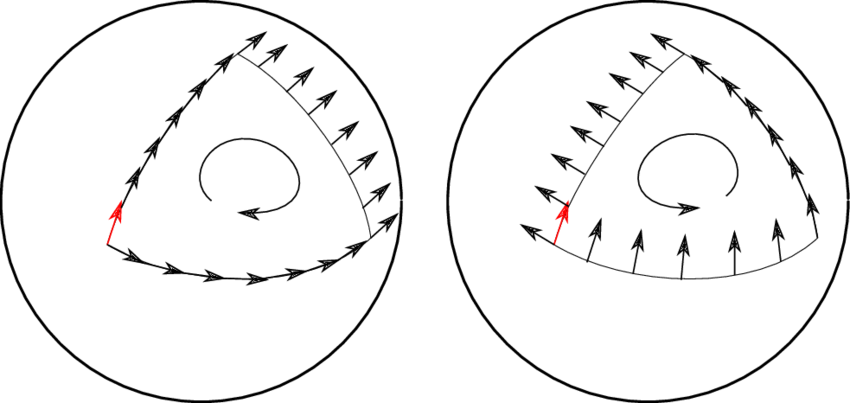
\includegraphics[width=0.60\textwidth]{parallel-transport.png}
	\caption{Parallel transport on a sphere.}
	\label{par-tr}
\end{figure}

\begin{proposition}
	La condizione di trasporto parallello di un campo vettoriale $ \ve{F}(\ve{x}) $ è che lungo la curva considerata si abbia $ \ve{e}^k \cdot d\ve{F} = 0 $.
\end{proposition}
Dato che $ d\ve{F} = \pa_l \ve{F} dx^l $, questa condizione è equivalente a richiedere che $ \nabla_l F^k = 0 $ lungo la curva.

\section{Derivata covariante}

Si introduce la seguente notazione per la derivata: $ f_{,i} = \frac{\pa f}{\pa x^i} $, indipendentemente dalla natura di $ f $.
Considerando un campo vettoriale $ \ve{F}(\ve{x}) $ su una varietà differenziabile $ \mathcal{M} $, quindi, si può riscrivere la derivata covariante come:
\begin{equation}
	\nabla_l F^k \equiv F^k_{;l} \defeq \ve{e}^k \cdot \ve{F}_{,l} = \ve{e}^k \cdot \left( F^i_{,l} \ve{e}_i + F^i \ve{e}_{i,l} \right) = F^k_{,l} + \Gamma^k_{li} F^i
	\label{eq:4.7}
\end{equation}

\begin{proposition}
	$ \ve{e}_k \cdot \ve{e}^i_{,l} = - \Gamma^i_{lk} $.
\end{proposition}
\begin{proof}
	$ 0 = \delta^i_{k,l} = \left( \ve{e}_k \cdot \ve{e}^i \right)_{,l} = \ve{e}_{k,l} \cdot \ve{e}^i + \ve{e}_k \cdot \ve{e}^i_{,l} = \Gamma^i_{lk} + \ve{e}_k \cdot \ve{e}^i_{,l} $.
\end{proof}
È dunque possibile esprimere la derivata covariante sia di un campo controvariante che di un campo covariante:
\begin{equation}
	V^k_{;l} \defeq \ve{e}^k \cdot \ve{V}_{,l} = \ve{e}^k \cdot \left( V^i_{,l} \ve{e}_i + V^i \ve{e}_{i,l} \right)
	\label{eq:4.8}
\end{equation}
\begin{equation}
	V_{k;l} \defeq \ve{e}_k \cdot \ve{V}_{,l} = \ve{e}_k \cdot \left( V_{i,l} \ve{e}^i + V_i \ve{e}^i_{,l} \right)
	\label{eq:4.9}
\end{equation}
Scrivendo in funzione delle connessioni affini:
\begin{equation}
	\nabla_l V^k = \frac{\pa V^k}{\pa x^l} + \Gamma^k_{li} V^i
	\label{eq:4.10}
\end{equation}
\begin{equation}
	\nabla_l V_k = \frac{\pa V_k}{\pa x^l} - \Gamma^i_{lk} V_i
	\label{eq:4.11}
\end{equation}
Sulle varietà torsion-free ($ T^a_{bc} \equiv 0 $) si può definire il rotore covariante come $ V_{l;i} - V_{i;l} = V_{l,i} - V_{i,l} $.

\begin{proposition}
	La derivata covariante trasforma come un tensore.
\end{proposition}
\begin{proof}
	Ricordando Eq. \ref{eq:4.6}:
	\begin{equation*}
		\begin{split}
			\tilde{\nabla}_l \tilde{V}^k
			&= \frac{\pa \tilde{V}^k}{\pa y^l} + \tilde{\Gamma}^k_{li}\tilde{V}^i = \frac{\pa x^m}{\pa y^l} \frac{\pa}{\pa x^m} \left( \frac{\pa y^k}{\pa x^p} V^p \right) + \tilde{\Gamma}^k_{lj} \tilde{V}^j\\
			&= \frac{\pa x^m}{\pa y^l} \frac{\pa y^k}{\pa x^p} \frac{\pa V^p}{\pa x^m} + \frac{\pa x^m}{\pa y^l} \frac{\pa^2 y^k}{\pa x^m \pa x^n} V^n + \frac{\pa y^k}{\pa x^p} \frac{\pa x^m}{\pa y^l} \underbrace{\frac{\pa x^n}{\pa y^j} \frac{\pa y^j}{\pa x_i}}_{\delta^n_i} \Gamma^p_{mn} V^i + \frac{\pa y^k}{\pa x^p} \frac{\pa^2 x^p}{\pa y^l \pa y^j} \frac{\pa y^j}{\pa x^n} V^n\\
			&= \frac{\pa x^m}{\pa y^l} \frac{\pa y^k}{\pa x^p} \left( \frac{\pa V^p}{\pa x^m} + \Gamma^p_{mn} V^n \right) + \left( \frac{\pa x^m}{\pa y^l} \frac{\pa^2 y^k}{\pa x^m \pa x^n} + \frac{\pa y^k}{\pa x^p} \frac{\pa^2 x^p}{\pa y^l \pa y^j} \frac{\pa y^j}{\pa x^n} \right) V^n
		\end{split}
	\end{equation*}
	Basta mostrare che il secondo termine è nullo:
	\begin{equation*}
		\begin{split}
			\frac{\pa}{\pa y^l} \frac{\pa y^k}{\pa x^n} + \frac{\pa y^k}{\pa x^p} \left[ \frac{\pa y^j}{\pa x^n} \frac{\pa}{\pa y^l} \frac{\pa x^p}{\pa y^j} \right]
			&= \frac{\pa}{\pa y^l} \frac{\pa y^k}{\pa x^n} + \frac{\pa y^k}{\pa x^p} \left[ \frac{\pa}{\pa y^l} \left( \frac{\pa y^j}{\pa x^n} \frac{\pa x^p}{\pa y^j} \right) - \frac{\pa x^p}{\pa y^j} \frac{\pa}{\pa y^l} \frac{\pa y^j}{\pa x^n} \right]\\
			&= \frac{\pa}{\pa y^l} \frac{\pa y^k}{\pa x^n} + \frac{\pa y^k}{\pa x^p} \left( \frac{\pa}{\pa y^l} \delta^p_n \right) - \delta^k_j \frac{\pa}{\pa y^l} \frac{\pa y^j}{\pa x^n} = \frac{\pa}{\pa y^l} \frac{\pa y^k}{\pa x^n} - \frac{\pa}{\pa y^l} \frac{\pa y^k}{\pa x^n} = 0
		\end{split}
	\end{equation*}
	Il caso della derivata covariante di un vettore covariante è analogo.
\end{proof}

\begin{proposition}\label{cov-2}
	La derivata covariante di un tensore di rango 2 è:
	\begin{equation}
		\nabla_k A_{ij} = \frac{\pa A_{ij}}{\pa x^k} - \Gamma^m_{ik} A_{mj} - \Gamma^m_{jk} A_{im}
		\label{eq:4.12}
	\end{equation}
	\begin{equation}
		\nabla_k A^{ij} = \frac{\pa A^{ij}}{\pa x^k} + \Gamma^i_{mk} A^{mj} + \Gamma^j_{mk} A^{im}
		\label{eq:4.13}
	\end{equation}
\end{proposition}
\begin{proof}
	$ \tens{A} = A_{ij} \ve{e}^i \otimes \ve{e}^j $, quindi:
	\begin{equation*}
		\begin{split}
			\frac{\pa \tens{A}}{\pa x^k}
			&= \frac{\pa A_{ij}}{\pa x^k} \ve{e}^i \otimes \ve{e}^j + A_{ij} \frac{\pa\ve{e}^i}{\pa x^k} \otimes \ve{e}^j + A_{ij} \ve{e}^i \otimes \frac{\pa\ve{e}^j}{\pa x^k}\\
			&= \frac{\pa A_{ij}}{\pa x^k} \ve{e}^i \otimes \ve{e}^j - A_{ij} \Gamma^i_{mk} \ve{e}^m \otimes \ve{e}^j - A_{ij} \Gamma^j_{mk} \ve{e}^i \otimes \ve{e}^m\\
			&= \frac{\pa A_{ij}}{\pa x^k} \ve{e}^i \otimes \ve{e}^j - A_{mj} \Gamma^m_{ik} \ve{e}^i \otimes \ve{e}^j - A_{im} \Gamma^m_{jk} \ve{e}^i \otimes \ve{e}^j\\
			&= \left( \frac{\pa A_{ij}}{\pa x^k} - \Gamma^m_{ik} A_{mj} - \Gamma^m_{jk} A_{im} \right) \ve{e}^i \otimes \ve{e}^j \eqdef \left( \nabla_k A_{ij} \right) \ve{e}^i \otimes \ve{e}^j
		\end{split}
	\end{equation*}
\end{proof}

\begin{proposition}
	Dato $ A_{ij} $ tensore di rango 2 antisimmetrico su una varietà torsion-free, si ha:
	\begin{equation}
		A_{ij;k} + A_{ki;j} + A_{jk;i} = A_{ij,k} + A_{ki,j} + A_{jk,i}
		\label{eq:4.14}
	\end{equation}
\end{proposition}
\begin{proof}
	Dalla Prop. \ref{cov-2}:
	\begin{equation*}
		\begin{split}
			A_{ij;k} + A_{ki;j} + A_{jk;i}
			&= A_{ij,k} - \Gamma^m_{ik} A_{mj} - \Gamma^m_{jk} A_{im} + A_{ki,j} - \Gamma^m_{kj} A_{mi} - \Gamma^m_{ij} A_{km} \\ &\qquad \qquad \qquad \qquad \qquad \qquad \qquad \qquad + A_{jk,i} - \Gamma^m_{ji} A_{mk} - \Gamma^m_{ki} A_{jm}
		\end{split}
	\end{equation*}
	Per simmetria di $ \Gamma^m_{ik} $ ed antisimmetria di $ A_{ij} $:
	\begin{equation*}
		\Gamma^m_{ik} A_{mj} = - \Gamma^m_{ki} A_{jk} \qquad \Gamma^m_{jk} A_{im} = - \Gamma^m_{kj} A_{mi} \qquad \Gamma^m_{ij} A_{km} = - \Gamma^m_{ji} A_{mk}
	\end{equation*}
	da cui segue la tesi.
\end{proof}

Ciò dimostra che l'identità di Bianchi è valida in qualsiasi sistema di riferimento su una varietà torsion-free.

\subsection{Varietà torsion-free}

\subsubsection{Connessioni affini}

\begin{definition}
	Si definisce \textit{simbolo di Christoffel del primo tipo} $ \Gamma_{ijk} \defeq g_{im} \Gamma^m_{jk} $.
\end{definition}

\begin{proposition}
	Su una varietà torsion-free $ \Gamma_{ijk} = \Gamma_{ikj} $.
\end{proposition}
\begin{proof}
	Banale ricordando che su una varietà torsion-free $ \Gamma^m_{jk} = \Gamma^m_{kj} $.
\end{proof}

\begin{proposition}\label{chri-1-2}
	$ \Gamma^m_{ij} = g^{km} \Gamma_{kij} $.
\end{proposition}
\begin{proof}
	$ g^{km} \Gamma_{kij} = g^{km} g_{kn} \Gamma^n_{ij} = \delta^m_n \Gamma^n_{ij} = \Gamma^m_{ij} $.
\end{proof}

È possibile esprimere le connessioni affini in funzione del tensore metrico.

\begin{proposition}\label{chri-1}
	$ \Gamma_{ijk} = \frac{1}{2} \left( g_{ij,k} + g_{ki,j} - g_{jk,i} \right) $.
\end{proposition}
\begin{proof}
	Si vede innanzitutto che $ \Gamma_{ijk} = g_{im} \Gamma^m_{jk} = g_{im} \ve{e}^m \cdot \ve{e}_{k,j} = \ve{e}_i \cdot \ve{e}_{k,j} $. Di conseguenza $ g_{ij,k} = \ve{e}_{i,k} \cdot \ve{e}_j + \ve{e}_i \cdot \ve{e}_{j,k} = \Gamma_{jki} + \Gamma_{ikj} $, ed analogamente $ g_{ki,j} = \Gamma_{ijk} + \Gamma_{kji} $ e $ g_{jk,i} = \Gamma_{kij} + \Gamma_{jik} $, dunque:
	\begin{equation*}
		\begin{split}
			g_{ij,k} + g_{ki,j} - g_{jk,i}
			&= \Gamma_{jki} + \Gamma_{ikj} + \Gamma_{ijk} + \Gamma_{kji} - \Gamma_{kij} - \Gamma_{jik}\\
			&= \Gamma_{jik} - \Gamma_{ijk} + \Gamma_{ijk} + \Gamma_{kij} - \Gamma_{kij} - \Gamma_{jik} = 2 \Gamma_{ijk}
		\end{split}
	\end{equation*}
\end{proof}

\begin{proposition}
	$ \Gamma^m_{ij} = \frac{1}{2} g^{km} \left( g_{ki,j} + g_{jk,i} - g_{ij,k} \right) $.
\end{proposition}
\begin{proof}
	Dalle Prop. \ref{chri-1-2} - \ref{chri-1}.
\end{proof}

\subsubsection{Derivata covariante del tensore metrico}

Dalla Prop. \ref{cov-2} si ha che:
\begin{equation}
	\nabla_k g_{ij} = \frac{\pa g_{ij}}{\pa x^k} - \Gamma^m_{ik} g_{mj} - \Gamma^m_{jk} g_{im}
	\label{eq:4.15}
\end{equation}
Dunque:
\begin{equation*}
	\begin{split}
		g_{ij;k}
		&= g_{ij,k} - \Gamma_{jik} - \Gamma_{ijk}\\
		&= g_{ij,k} - \frac{1}{2} \left( g_{ji,k} + g_{kj,i} - g_{ik,j} \right) - \frac{1}{2} \left( g_{ij,k} + g_{ki,j} - g_{jk,i} \right)\\
		&= g_{ij,k} - \frac{1}{2} g_{ijk,k} + \frac{1}{2} g_{jk,i} + \frac{1}{2} g_{ik,j} - \frac{1}{2} g_{ij,k} - \frac{1}{2} g_{ik,j} + \frac{1}{2} g_{jk,i} = 0
	\end{split}
\end{equation*}
Si vede quindi una delle proprietà fondamentali delle varietà torsion-free, ovvero la preservazione della metrica:
\begin{equation}
	\nabla_k g_{ij} = 0
	\label{eq:4.16}
\end{equation}

\section{Operatori differenziali su varietà curve}

Considerata una generica varietà differenziabile $ n $-dimensionale $ \mathcal{M} $, fissando un RF $ \{\ve{e}_i\}_{i = 1, \dots, n} $ ortogonale, è possibile definire su $ \mathcal{M} $ gli usuali operatori differenziali dello spazio euclideo.

\subsection{Gradiente}

\begin{definition}
	Dato  un campo scalare $ f : \mathcal{M} \rightarrow \R $, si definisce il suo differenziale come:
	\begin{equation}
		df(\ve{x}) = f(\ve{x} + d\ve{x}) - f(\ve{x}) = \frac{\pa f}{\pa x^i}dx^i \eqdef \nabla f(\ve{x}) \cdot d\ve{x}
		\label{eq:4.17}
	\end{equation}
\end{definition}

\begin{proposition}
	$ \nabla f = \displaystyle\sum_{i = 1}^{n} \frac{1}{h_i} \frac{\pa f}{\pa x^i} \hat{\ve{e}}_i $.
\end{proposition}
\begin{proof}
	Dato che $ \frac{\hat{\ve{e}}_i}{h_i} = \ve{e}^i $ (giustamente $ \frac{\pa f}{\pa x^i} $ è covariante):
	\begin{equation*}
		\nabla f \cdot d\ve{x} = \frac{\pa f}{\pa x^i} \ve{e}^i \cdot dx^j \ve{e}_j = \frac{\pa f}{\pa x^i} dx^j \delta^j_i = \frac{\pa f}{\pa x^i} dx^i = df
	\end{equation*}
\end{proof}

\subsection{Divergenza}

\begin{definition}
	Dato un campo vettoriale controvariante $ \ve{V} = V^i \ve{e}_i $, si definisce la sua divergenza come:
	\begin{equation}
		\nabla\cdot\ve{V} \defeq V^i_{;i} = V^i_{,i} + \Gamma^i_{ik} V^k
		\label{eq:4.18}
	\end{equation}
\end{definition}

La divergenza non è altro che una contrazione della derivata covariante.

\begin{proposition}\label{chri-contr}
	$ \Gamma^i_{ik} = \frac{1}{2} g^{im} g_{im,k} $.
\end{proposition}
\begin{proof}
	$ \Gamma^i_{ik} = \frac{1}{2} g^{im} \left( g_{im,k} + g_{ki,m} - g_{mk,i} \right) $, ma $ g^{im} g_{mk,i} = g^{mi} g_{ik,m} $ poichè $ m $, $ i $ indici muti, da cui la tesi.
\end{proof}

È possibile dare una formulazione alternativa. Si ricordi che, definendo $ c $ la matrice dei cofattori del tensore metrico $ g $ (visto come matrice):
\begin{equation}
	\det g = \sum_{i,j} g_{ij} c_{ij} \quad \Longrightarrow \quad c_{ij} = \frac{\pa\det g}{\pa g_{ij}}
	\label{eq:4.19}
\end{equation}
Ricordando poi che $ \left( g_{ij} \right)^{-1} = \left( \det g \right)^{-1} c_{ij} $:
\begin{equation}
	g^{ij} = \frac{1}{\det g} \frac{\pa\det g}{\pa g_{ij}}
	\label{eq:4.20}
\end{equation}

\begin{proposition}\label{chri-g}
	$ \Gamma^i_{ik} = \frac{\left( \sqg \right)_{,k}}{\sqg} $.
\end{proposition}
\begin{proof}
	Innanzitutto $ \left( \det g \right)_{,k} = g_{ij,k} \frac{\pa\det g}{\pa g_{ij}} = g_{ij,k} g^{ij} \det g $, quindi, dalla Prop. \ref{chri-contr}:
	\begin{equation*}
		\Gamma^i_{ik} = \frac{1}{2} g^{im} g_{im,k} = \frac{1}{2} \frac{1}{\det g} \left( \det g \right)_{,k} = \frac{1}{2\abs{\det g}} \abs{\det g}_{,k} \equiv \frac{\tens{g}_{,k}}{2\tens{g}} = \frac{\left( \sqg \right)_{,k}}{\sqg}
	\end{equation*}
\end{proof}

\begin{proposition}\label{dive-cov}
	Dato un campo vettoriale controvariante $ \ve{V} = V^i \ve{e}_i $, la sua divergenza è:
	\begin{equation}
		\nabla\cdot\ve{V} = \frac{\left( \sqg V^k \right)_{,k}}{\sqg}
		\label{eq:4.21}
	\end{equation}
\end{proposition}
\begin{proof}
	Dalle Prop. \ref{chri-g}:
	\begin{equation*}
		\nabla\cdot\ve{V} = V^i_{,i} + \Gamma^i_{ik} V^k = V^i_{,i} + \frac{\left( \sqg \right)_{,k}}{\sqg} V^k = \frac{\left( \sqg V^k \right)_{,k}}{\sqg}
	\end{equation*}
\end{proof}

\begin{definition}
	Si definisce la \textit{delta di Kronecker generalizzata} come:
	\begin{equation}
		\delta^{\mu_1 \dots \mu_k}_{\nu_1 \dots \nu_k} \defeq
		\begin{cases}
			+1 & (\nu_1,\dots,\nu_k) = \sigma_p (\mu_1,\dots,\mu_k) \text{ distinti} \\
			-1 & (\nu_1,\dots,\nu_k) = \sigma_d (\mu_1,\dots,\mu_k) \text{ distinti} \\
			0 & \text{altrimenti}
		\end{cases}
		\label{eq:4.22}
	\end{equation}
\end{definition}
\begin{lemma}
	Si ha:
	\begin{equation}
		\delta^{\mu_1 \dots \mu_k}_{\nu_1 \dots \nu_k} = \det
		\begin{bmatrix}
			\delta^{\mu_1}_{\nu_1} & \dots & \delta^{\mu_1}_{\nu_k}\\
			\vdots & \ddots & \vdots\\
			\delta^{\mu_k}_{\nu_1} & \dots & \delta^{\mu_k}_{\nu_k}
		\end{bmatrix}
		\label{eq:4.23}
	\end{equation}
\end{lemma}
\begin{lemma}\label{eps-gen}
	$ \epsilon_{i_1 \dots i_k i_{k+1} \dots i_n} \epsilon^{i_i \dots i_k j_{k+1} \dots j_n} = k! \delta^{j_{k+1} \dots j_n}_{i_{k+1} \dots i_n} $.
\end{lemma}

\begin{proposition}
	Dato un campo vettoriale $ \ve{V} = V^i \ve{e}_i $, detta $ V = V_i dx^i $ la forma differenziale ad esso associata, si ha:
	\begin{equation}
		\nabla\cdot\ve{V} = \sigma * d * V
		\label{eq:4.24}
	\end{equation}
\end{proposition}
\begin{proof}
	Per semplicità si considera il caso 4-dimensionale (si usa il Lemma \ref{eps-gen}):
	\begin{equation*}
		\begin{split}
			*d*V
			&= *d \left( V_i \frac{1}{3!} g^{ik} \varepsilon_{klmn} dx^l \wedge dx^m \wedge dx^n \right) = * \left[ \frac{1}{3!} \left( \sqg V^k \right)_{,p} \epsilon_{klmn} dx^p \wedge dx^l \wedge dx^m \wedge dx^n \right]\\
			&= \frac{1}{3!} \left( \sqg V^k \right)_{,p} \epsilon_{klmn} *\left( dx^p \wedge dx^l \wedge dx^m \wedge dx^n \right) = \frac{1}{3!} \left( \sqg V^k \right)_{,p} \epsilon_{klmn} g^{p \alpha} g^{l \beta} g^{m \gamma} g^{n \delta} \sqg \epsilon_{\alpha \beta \gamma \delta}\\
			&= \frac{1}{3!} \left( \sqg V^k \right)_{,p} \sqg \epsilon_{klmn} \left( \det g \right)^{-1} \epsilon^{plmn} = \frac{1}{3!} \frac{\sigma}{\sqg} \left( \sqg V^k \right)_{,p} \left( 3! \delta^p_k \right) = \frac{\sigma}{\sqg} \left( \sqg V^k \right)_{,k}
		\end{split}
	\end{equation*}
\end{proof}

\begin{example}
	In uno spazio piatto $ n $-dimensionale con $ g_{ij} = h_i^2 \delta_{ij} $ si ha $ \bar{V}_i \equiv h_i^{-1} V_i = h_i V^i $, quindi:
	\begin{equation*}
		\nabla\cdot\ve{V} = \frac{1}{\sqrt{h_1^2 \dots h_n^2}} \sum_{k = 1}^{n} \left( \sqrt{h_1^2 \dots h_n^2} \bar{V}_k \right)_{,k} = \frac{1}{h_1 \dots h_n} \sum_{k = 1}^{n} \frac{\pa}{\pa x^k} \left( \frac{h_1 \dots h_n}{h_k} V_k \right)
	\end{equation*}
\end{example}

\subsection{Laplaciano}

\begin{definition}
	Dato un campo scalare $ f : \mathcal{M} \rightarrow \R $, si definisce il suo laplaciano come:
	\begin{equation}
		\Box f \defeq \nabla\cdot\nabla f = \left( g^{ik} f_{,k} \right)_{;i}
		\label{eq:4.25}
	\end{equation}
\end{definition}

% Nella letteratura russa è indicato anche con $ \Delta $, mentre in uno spazio piatto con $ \nabla^2 $.

\begin{proposition}
	Si ha:
	\begin{equation}
		\Box f = \frac{\left( \sqg f^{,k} \right)_{,k}}{\sqg}
		\label{eq:4.26}
	\end{equation}
\end{proposition}
\begin{proof}
	Banale dalla Prop. \ref{dive-cov}, usando $ g^{ik} f_{,k} = f^{,i} $.
\end{proof}

\begin{proposition}
	Dato un campo scalare $ f : \mathcal{M} \rightarrow \R $, si ha:
	\begin{equation}
		\Box f = \sigma * d * df
		\label{eq:4.27}
	\end{equation}
\end{proposition}
\begin{proof}
	\begin{equation*}
		\begin{split}
			*d*df
			&= *d \left( f_{,i} *dx^i \right) = *d \left( \frac{1}{3!} \sqg f_{,i} g^{ik} \epsilon_{klmn} dx^l \wedge dx^m \wedge dx^n \right)\\
			&= * \left( \frac{1}{3!} \left( \sqg f^{,k} \right)_{,p} \epsilon_{klmn} dx^p \wedge dx^l \wedge dx^m \wedge dx^n \right)\\
			&= \frac{1}{3!} \left( \sqg f^{,k} \right)_{,p} \epsilon_{klmn} g^{p \alpha} g^{l \beta} g^{m \gamma} g^{n \delta} \sqg \epsilon_{\alpha \beta \gamma \delta}\\
			&= \frac{1}{3!} \left( \sqg f^{,k} \right)_{,p} \epsilon_{klmn} \sqg \left( \det g \right)^{-1} \epsilon^{plmn} = \frac{1}{3!} \frac{\sigma}{\sqg} \left( \sqg f^{,k} \right)_{,p} 3! \delta^p_k = \frac{\sigma}{\sqg} \left( \sqg f^{,k} \right)_{,k}
		\end{split}
	\end{equation*}
\end{proof}

\begin{example}
	In uno spazio piatto $ n $-dimensionale con $ g_{ij} = h_i^2 \delta_{ij} $ si ha $ f^{,k} = g^{ik} f_{,i} = h_k^{-2} f_{,k} $, quindi:
	\begin{equation*}
		\nabla^2 f = \frac{1}{\sqrt{h_1^2 \dots h_n^2}} \sum_{k = 1}^{n} \left( \sqrt{h_1^2 \dots h_n^2} h_k^{-2} f_{,k} \right)_{,k} = \frac{1}{h_1 \dots h_n} \sum_{k = 1}^{n} \frac{\pa}{\pa x^k} \left( \frac{h_1 \dots h_n}{h_k^2} \frac{\pa f}{\pa x^k} \right)
	\end{equation*}
\end{example}

\section{Elettrodinamica covariante}

Riprendendo il potenziale \ref{eq:2.21}, è possibile definire la 1-form $ A = A_i dx^i $:

\begin{equation}
	dA = \pa_i A_j dx^i \wedge dx^j = \frac{1}{2} F_{ij} dx^i \wedge dx^j \equiv F
	\label{eq:3.13}
\end{equation}

dove è stata definita la 2-form determinata dal tensore di Faraday \ref{eq:2.23}. L'Eq. \ref{eq:2.25} diventa, grazie all'identità di Bianchi:

\begin{equation}
	dF = 0
	\label{eq:3.14}
\end{equation}

Nel caso elettrostatico $ \dot{\ve{B}} = 0 $, quindi $ \nabla\times\ve{E} = 0 $, ovvero $ dE = 0 $: il campo elettrostatico è chiuso e, per il teorema di Stokes, localmente esatto.\\
È anche possibile calcolare il duale di Hodge di $ F $:
\begin{equation}
	*F = \frac{1}{2}F_{ij} * \left( dx^i \wedge dx^j \right) = \frac{1}{4} F_{ij} g^{ik} g^{il} \varepsilon_{klmn} dx^m \wedge dx^n = \frac{1}{4} F^{kl} \varepsilon_{klmn} dx^m \wedge dx^n
	\label{eq:3.22}
\end{equation}
Applicando il duale della derivata esteriore:
\begin{equation}
	\begin{split}
		*d*F &= \frac{1}{4} \pa_p \left( F^{kl} \varepsilon_{klmn} \right) * \left( dx^p \wedge dx^m \wedge dx^n \right) = \frac{1}{4} \pa_p \left( \sqg F^{kl} \right) \epsilon_{klmn} g^{p\alpha} g^{m\beta} g^{n\gamma} \varepsilon_{\alpha\beta\gamma\delta} dx^{\delta}\\
		     &= \frac{1}{4} \pa_p \left( \sqg F^{kl} \right) \sqg \, \epsilon_{klmn} g^{\alpha p} g^{\beta m} g^{\gamma n} g^{\delta w} \epsilon_{\alpha\beta\gamma\delta} dx_w = \frac{1}{4} \pa_p \left( \sqg F^{kl} \right) \sqg\, \epsilon_{klmn} \frac{\sigma}{\tens{g}} \epsilon^{pmnw} dx_w\\
		     &= \frac{1}{4} \pa_p \left( \sqg F^{kl} \right) \frac{\sigma}{\sqg} 2 \left( \delta^p_k \delta^w_l - \delta^w_k \delta^p_l \right) dx_w = \frac{\sigma}{2\sqg} \left[ \pa_p \left( \sqg F^{pw} \right) dx_w - \pa \left( \sqg F^{wp} \right) dx_w \right]\\
		     &= - \frac{\sigma}{\sqg} \pa_p \left( \sqg F^{kp} \right) dx_k
	\end{split}
	\label{eq:3.23}
\end{equation}
Nello spaziotempo di Minkowski $ g_{ij} = \diag(-1,1,1,1) $, dunque l'Eq. \ref{eq:3.23} si riduce a $ *d*F = \pa_p (F^{kp}) dx_k $: ricordando dall'Eq. \ref{eq:2.27} che $ \pa_p (F^{kp}) = \mu_0 j^k $, definendo la 1-form della corrente $ j \defeq j^k dx_k $ si trova la generalizzazione su varietà curva della seconda equazione di Maxwell covariante:
\begin{equation}
	*d*F = \mu_0 j
	\label{eq:3.24}
\end{equation}
Questa, unità all'identità di Bianchi Eq. \ref{eq:3.14}, rappresenta tutti i fenomeni dell'elettrodinamica classica.












\chapter{Relatività Generale}
\selectlanguage{italian}

\section{Principio d'azione stazionaria}

\subsection{Caso classico}

\begin{definition}
	Dato un sistema descritto da una lagrangiana $ L $, si definisce l'azione come:
	\begin{equation}
		S[\ve{x}(t)] \defeq \int_{t_1}^{t_2} L(\ve{x}, \dot{\ve{x}}) dt
		\label{eq:5.1}
	\end{equation}
\end{definition}

Il principio di minima azione afferma che la traiettoria percorsa dal sistema è un estremante dell'azione, ovvero, considerata una variazione della traiettoria $ \delta\ve{x} : \delta\ve{x}(t_1) = \delta\ve{x}(t_2) = \ve{0} $:
\begin{equation}
	\delta S = 0
	\label{eq:5.2}
\end{equation}

\subsubsection{Particella libera}

Classicamente, una particella libera è descritta da $ L = \frac{1}{2} m \dot{\ve{x}}^2 $, dunque:
\begin{equation*}
	\begin{split}
		0
		&= \delta S = \int_{t_1}^{t_2} \delta L \,dt = \int_{t_1}^{t_2} m \dot{\ve{x}} \cdot \delta\dot{\ve{x}} \,dt = \int_{t_1}^{t_2} \left[ m \frac{d}{dt} \left( \dot{\ve{x}} \cdot \delta\ve{x} \right) - m \ddot{\ve{x}} \cdot \delta\ve{x} \right] dt\\
		&= m \left[ \ddot{\ve{x}} \cdot \delta\ve{x} \right]_{t_1}^{t_2} - m \int_{t_1}^{t_2} \ddot{\ve{x}} \cdot \delta\ve{x} \,dt = -m \int_{t_1}^{t_2} \ddot{\ve{x}} \cdot \delta\ve{x} \,dt
	\end{split}
\end{equation*}
Dunque, data l'arbitrarietà di $ \delta\ve{x} $, si ha l'equazione del moto della particella libera classica:
\begin{equation}
	\ddot{\ve{x}} = \ve{0}
	\label{eq:5.3}
\end{equation}

\subsubsection{Moto in un potenziale}

In presenza di un potenziale, la lagrangiana diventa $ L = \frac{1}{2} m \dot{\ve{x}}^2 - V(\ve{x}) $, quindi, dato che $ \delta V(\ve{x}) = \nabla V(\ve{x}) \cdot \delta\ve{x} $, si ha l'equazione del moto:
\begin{equation}
	0 = \delta S = \int_{t_1}^{t_2} \left( - m\ddot{\ve{x}} - \nabla V(\ve{x}) \right) \cdot \delta\ve{x} \,dt \quad\Longrightarrow\quad m\ddot{\ve{x}} = - \nabla V(\ve{x})
	\label{eq:5.4}
\end{equation}

\subsection{Caso relativistico}

\begin{proposition}
	Una particella libera relativistica è descritta da $ L = - \frac{m c^2}{\gamma} $.
\end{proposition}
\begin{proof}
	$ p_i = \frac{\pa L}{\pa v_i} = - mc^2 \frac{\pa}{\pa v_i} \sqrt{1 - \frac{\ve{v}^2}{c^2}} = -mc^2 \left( -  \gamma \frac{v_i}{c} \right) = \gamma m v_i $, ovvero $ \ve{p} = \gamma m \ve{v} $.
\end{proof}

\subsubsection{Particella libera}

L'azione che descrive una particella libera relativistica è:
\begin{equation}
	S = - mc^2 \int_{t_1}^{t_2} \frac{dt}{\gamma} = -mc \int_{\tau_1}^{\tau_2} d\tau
	\label{eq:5.5}
\end{equation}
Ponendo $ c = 1 $, è possibile calcolare le equazioni del moto:
\begin{equation*}
	\begin{split}
		0
		&= \delta S = - \delta \int_{t_1}^{t_2} m \sqrt{1 - \dot{\ve{x}}^2} \,dt = m \int_{t_1}^{t_2} \frac{\dot{\ve{x}} \cdot \delta\dot{\ve{x}}}{\sqrt{1 - \dot{\ve{x}}^2}} dt = m \int_{t_1}^{t_2} \frac{d\ve{x}}{dt} \cdot \frac{d \delta\ve{x}}{dt} \frac{dt}{d\tau} \,dt\\
		&= m \int_{\tau_1}^{\tau_2} \frac{d\ve{x}}{dt} \cdot \frac{d \delta\ve{x}}{dt} \frac{dt}{d\tau} \frac{dt}{d\tau} \,d\tau = m \int_{\tau_1}^{\tau_2} \frac{d\ve{x}}{d\tau} \cdot \frac{d\delta\ve{x}}{d\tau} \,d\tau\\
		&= m \int_{\tau_1}^{\tau_2} \left[ \frac{d}{d\tau} \left( \dot{\ve{x}} \cdot \delta\ve{x} \right) - \frac{d^2\ve{x}}{d\tau^2} \cdot \delta\ve{x} \right] d\tau = - m \int_{\tau_1}^{\tau_2} \frac{d^2 \ve{x}}{d\tau^2} \cdot \delta\ve{x} \,d\tau
	\end{split}
\end{equation*}
Dall'arbitrarietà di $ \delta\ve{x} $ si ottiene l'equazione del moto:
\begin{equation}
	\frac{d^2 \ve{x}}{d\tau^2} = \ve{0}
	\label{eq:5.6}
\end{equation}

\subsubsection{Campo elettromagnetico}

Per descrivere il moto di una particella in un campo elettromagnetico, è necessario aggiungere un termine d'interazione alla lagrangiana:
\begin{equation}
	S = -m \int_{\tau_1}^{\tau_2} d\tau + q \int_{\ve{x}_1}^{\ve{x}_2} A_i(\ve{x}) dx^i = \int_{\tau_1}^{\tau_2} \left( -m + q A_i (\ve{x}) \frac{dx^i}{d\tau} \right) d\tau
	\label{eq:5.7}
\end{equation}
Per ottenere le equazioni del moto, dunque:
\begin{equation*}
	\begin{split}
		0
		&= \delta S = -m \int_{\tau_1}^{\tau_2} \delta\sqrt{-\eta_{ij} dx^i dx^j} + q \int_{\ve{x}_1}^{\ve{x}_2} \delta \left( A_i dx^i \right)\\
		&= -m \int_{\tau_1}^{\tau_2} \frac{1}{2} \frac{\delta \left( - \eta_{ij} dx^i dx^j \right)}{\sqrt{- \eta_{ij} dx^i dx^j}} + q \int_{\ve{x}_1}^{\ve{x}_2} \left( \delta A_i dx^i + A_i \delta dx^i \right)\\
		&= m \int_{\tau_1}^{\tau_2} \frac{1}{2} \frac{\eta_{ij} \left( \delta dx^i dx^j + dx^i \delta dx^j \right)}{\sqrt{- \eta_{ij} dx^i dx^j}} + q \int_{\tau_1}^{\tau_2} \left( \delta A_i \frac{dx^i}{d\tau} + A_i \frac{d\delta x^i}{d\tau} \right) d\tau\\
		&= \int_{\tau_1}^{\tau_2} \left( m \frac{\eta_{ij} dx^i}{\sqrt{- \eta_{ij} dx^i dx^j}} \frac{d\delta x^j}{d\tau} + q \frac{\pa A_i}{\pa x^k} \delta x^k \frac{dx^i}{d\tau} + q A_i \frac{d\delta x^i}{d\tau} \right) d\tau\\
		&= \int_{\tau_1}^{\tau_2} \left( m \eta_{ij} \frac{dx^i}{d\tau} \frac{d\delta x^j}{d\tau} + q A_{i,k} \delta x^k \frac{dx^i}{d\tau} + q A_i \frac{d\delta x^i}{d\tau} \right) d\tau\\
		&= \int_{\tau_1}^{\tau_2} \left( - m \frac{du_k}{d\tau} \delta x^k + q A_{i,k} u^i \delta x^k - q \frac{dA_k}{d\tau} \delta x^k \right) d\tau\\
		&= \int_{\tau_1}^{\tau_2} \left( -m \frac{du_k}{d\tau} + q \left( A_{i,k} - A_{k,i} \right) u^i \right) \delta x^k d\tau
	\end{split}
\end{equation*}
dove si è usata la quadrivelocità $ u_k $. Ricordando la definizione del tensore di Faraday $ F_{ij} \defeq A_{j,i} - A_{i,j} $, si trova l'espressione covariante della forza di Lorentz:
\begin{equation}
	\frac{dp_k}{d\tau} = q F_{ki} u^i
	\label{eq:5.8}
\end{equation}
Ciò conferma la scelta della lagrangiana.

\subsubsection{Campo gravitazionale}

Si consideri ora una particella su una varietà curva:
\begin{equation*}
	\begin{split}
		0
		&= \delta S = -m \int_{\tau_1}^{\tau_2} \delta d\tau = -m \int_{\tau_1}^{\tau_2} \delta \sqrt{- g_{ij} dx^i dx^j} = m \int_{\tau_1}^{\tau_2} \frac{1}{2} \frac{\delta g_{ij} dx^i dx^j + 2g_{ij} dx^i \delta dx^j}{\sqrt{- g_{ij} dx^i dx^j}}\\
		&= m \int_{\tau_1}^{\tau_2} \left( \frac{1}{2} g_{ij,k} u^i u^j \delta x^k d\tau + g_{ij} u^i \delta dx^j \right) = m \int_{\tau_1}^{\tau_2} \left( \frac{1}{2} g_{ij,k} u^i u^j \delta x^k + g_{ij} u^i \frac{d\delta x^j}{d\tau} \right) d\tau\\
		&= m \int_{\tau_1}^{\tau_2} \left( \frac{1}{2} g_{ij,k} u^i u^j \delta x^k - \frac{d}{d\tau} \left( g_{ij} u^i \right) \delta x^j \right) d\tau = m \int_{\tau_1}^{\tau_2} \left( \frac{1}{2} g_{ij,k} u^i u^j - \frac{d}{d\tau} \left( g_{ik} u^i \right) \right) \delta x^k d\tau
	\end{split}
\end{equation*}
Essendo $ \delta x^k $ arbitrario si ottiene:
\begin{equation}
	\frac{1}{2} g_{ij,k} u^i u^j - g_{ik,j} u^i u^j - g_{ik} \frac{du^i}{d\tau} = 0
	\label{eq:5.9}
\end{equation}
Moltiplicando per $ g^{rk} $:
\begin{equation}
	\frac{du^r}{d\tau} + g^{rk} \left( g_{ik,j} - \frac{1}{2} g_{ij,k} \right) u^i u^j = 0
	\label{eq:5.10}
\end{equation}
Dato che sopravvive solo la parte simmetrica rispetto a $ i,j $ del tensore moltiplicato per $ u^i u^j $:
\begin{equation}
	\frac{du^r}{d\tau} + \frac{1}{2} g^{rk} \left( g_{ik,j} + g_{jk,i} - g_{ij,k} \right) u^i u^j = 0
	\label{eq:5.11}
\end{equation}
Si vede la definizione di connessione di Levi-Civita (Eq. \ref{levi-civita}):
\begin{equation}
	\frac{d^2 x^r}{d\tau^2} + \Gamma^r_{ij} \frac{dx^i}{d\tau} \frac{dx^j}{d\tau} = 0
	\label{eq:5.12}
\end{equation}
Questa è nota come \textit{equazione geodetica} e descrive il moto di una particella libera su una varietà curva: si vede che, oltre al termine inerziale, è presente un termine di forza dovuto alla geometria stessa dello spazio; inoltre, si può osservare come la traiettoria sia indipendente dalla massa del corpo.
Sebbene la connessione di Levi-Civita non sia un tensore, si dimostra che il termine di forza annulla i termini non-omogenei, rendendo l'equazione geodesica un'equazione tensoriale.\\
In generale, le soluzioni dell'equazione geodetica sono dette geodetiche.
\begin{definition}
	Data una varietà differenziale $ \mathcal{M} $ e due punti $ p,q\in\mathcal{M} $, si dice \textit{geodetica} da $ p $ a $ q $ la curva di lunghezza minore tra $ p $ e $ q $.
\end{definition}
\begin{proposition}
	Dati una geodetica $ \gamma : I \subset \R \rightarrow \mathcal{M} $ ed il suo vettore tangente $ \ve{t}_{\gamma} $, si ha $ \frac{d\ve{t}_{\gamma}}{ds} = \ve{0} $.
\end{proposition}
\begin{proof}
	Ricordando che $ t^i = \frac{dx^i}{ds} $:
	\begin{equation*}
		\frac{d\ve{t}_{\gamma}}{ds} = t^i_{;k} \frac{dx^k}{ds} \ve{e}_i = \left( \frac{\pa t^i}{\pa x^k} + \Gamma^i_{jk} t^j \right) \frac{dx^k}{ds} \ve{e}_i = \left( \frac{d^2 x^i}{ds^2} + \Gamma^i_{jk} \frac{dx^j}{ds} \frac{dx^k}{ds} \right) \ve{e}_i = \ve{0}
	\end{equation*}
\end{proof}

\subsubsection{Campo elettromagnetico e gravitazionale}

Nel caso di una particella soggetta ad un campo elettromagnetico su una varietà curva:
\begin{equation}
	S = -m \int_{\tau_1}^{\tau_2} \sqrt{- g_{ij} dx^i dx^j} + q \int_{\tau_1}^{\tau_2} A_i \frac{dx^i}{d\tau} d\tau
	\label{eq:5.13}
\end{equation}
Svolgendo i calcoli, si trova l'equazione del moto:
\begin{equation}
	\frac{d^2 x^r}{d\tau^2} + \Gamma^r_{ij} \frac{dx^i}{d\tau} \frac{dx^j}{d\tau} - \frac{q}{m} F^r_{\,\,\,i} \frac{dx^i}{d\tau} = 0
	\label{eq:5.14}
\end{equation}
che conferma l'identificazione del termine geometrico con la forza di gravità.

\subsection{Principio d'equivalenza}

In presenza di un campo gravitazionale, dunque su una varietà curva, è possibile scegliere delle coordinate, dette free-fall coordinates, in cui, restringendosi ad una regione di spaziotempo sufficientemente piccola (così da poter trascurare localmente la curvatura, tutte le leggi fisiche hanno la stessa forma: ciò è possibile poiché, in tale regione, il tensore metrico può essere ricondotto con un cambio di RF alla metrica di Minkowski, dunque si recupera la fisica in spaziotempo piatto.\\
Perché ciò avvenga:
\begin{equation}
	\eta_{ij} = \frac{\pa x^k}{\pa y^i} \frac{\pa x^l}{\pa y^j} g_{kl} \quad\Longrightarrow\quad \eta = \tens{D}^{\intercal} g \tens{D}
	\label{eq:5.15}
\end{equation}
con $ \tens{D} = \tens{J}^{-1} $. Questa è una relazione di similitudine.\\
In tale RF, l'equazione del moto è quella della particella libera relativistica:
\begin{equation}
	\frac{d^2 y^i}{d \tau^2} = 0, \,\,\,\, d\tau^2 = - \eta_{ij} dx^i dx^j
	\label{eq:5.16}
\end{equation}
Queste coordinate sono anche dette coordiante libere o di Fermi.\\
È possibile recuperare l'equazione geodesica dall'Eq. \ref{eq:5.16}:
\begin{equation}
	0 = \frac{d}{d\tau} \left( \frac{\pa y^i}{\pa x^k} \frac{dx^k}{d\tau} \right) = \frac{\pa y^i}{\pa x^k} \frac{d^2 x^k}{d\tau^2} + \frac{\pa^2 y^i}{\pa x^l \pa x^k} \frac{dx^k}{d\tau} \frac{dx^l}{d\tau}
	\label{eq:5.17}
\end{equation}
Moltiplicando per $ \frac{\pa x^m}{\pa y^i} $:
\begin{equation}
	\frac{d^2 x^m}{d\tau^2} + \frac{\pa x^m}{\pa y^i} \frac{\pa^2 y^i}{\pa x^l \pa x^k} \frac{dx^k}{d\tau} \frac{dx^l}{d\tau}
	\label{eq:5.18}
\end{equation}
che corrisponde all'equazione geodetica ponendo:
\begin{equation}
	\Gamma^m_{kl} = \frac{\pa x^m}{\pa y^i} \frac{\pa^2 y^i}{\pa x^l \pa x^k}
	\label{eq:5.19}
\end{equation}
Questo poter approssimare localmente lo spaziotempo curvo con lo spaziotempo di Minkowski è il \textit{principio d'equivalenza di Einstein}.

\subsubsection{Principio d'equivalenza newtoniana}

Anche nella fisica newtoniana è presente un principio d'equivalenza. Si cosideri una particella massiva, descritta dall'equazione del moto:
\begin{equation}
	m_{\text{i}} \frac{d^2 \ve{x}}{dt^2} = m_{\text{g}} \ve{g} + \sum_{k} \ve{F}_k
	\label{eq:5.20}
\end{equation}
In questo caso, le coordinate free-fall sono definite da:
\begin{equation}
	\ve{y} = \ve{x} - \frac{1}{2} \ve{g} t^2
	\label{eq:5.21}
\end{equation}
In questo RF, l'equazione del moto diventa:
\begin{equation}
	m_{\text{i}} \left[ \frac{d^2\ve{y}}{dt^2} + \ve{g} \right] = m_{\text{g}} \ve{g} + \sum_{k} \ve{F}_k
	\label{eq:5.22}
\end{equation}
Il principio d'equivalenza newtoniano è un fatto sperimentale e afferma che:
\begin{equation}
	m_{\text{i}} = m_{\text{g}}
	\label{eq:5.23}
\end{equation}
Dunque, nel caso di una particella non soggetta ad altre forze, nelle coordinate free-fall l'equazione del moto diventa quella per la particella libera:
\begin{equation}
	\frac{d^2 \ve{y}}{dt^2} = \ve{0}
	\label{eq:5.24}
\end{equation}
Si vede dunque che le coordinate free-fall $ \virgolette{seguono} $ il moto del grave nel campo gravitazionale; in maniera analoga, le coordinate di Fermi individuano un RF che segue il moto della particella all'interno dello spaziotempo curvo.

\subsection{Campi gravitazionali deboli statici}

Le connessioni affini costituiscono una generalizzazione del campo di forza gravitazionale newtoniano, mentre il tensore metrico è una generalizzazione del potenziale gravitazionale newtoniano.\\
Per semplicità, si pongano le approssimazioni di campo debole (componenti spaziali trascurabili rispetto a quella temporale) e statico (derivate temporali trascurabili): l'equazione geodetica diventa:
\begin{equation}
	\frac{du^r}{d\tau} + \Gamma^r_{00} \left( u^0 \right)^2 = 0
	\label{eq:5.25}
\end{equation}
Dato che, nell'approssimazione fatta, $ g_{k0,0} = g_{0k,0} = 0 $, si ha $ \Gamma^r_{00} = -\frac{1}{2} g^{rk}g_{00,k} $. Nell'approssimazione di campo debole si può scrivere:
\begin{equation}
	g_{ij} = \eta_{ij} + h_{ij}, \quad \abs{h_{ij}} \ll 1
	\label{eq:5.26}
\end{equation}
Trascurando i termini $ o(h) $, si trova $ \Gamma^r_{00} = -\frac{1}{2} h_{00,r} $, con $ r = 1,2,3 $, quindi:
\begin{equation}
	\frac{d^2 x^r}{d\tau^2} = \frac{1}{2} \left( \frac{dx^0}{d\tau} \right)^2 h_{00,r} \quad\Longrightarrow\quad \frac{d^2 \ve{x}}{dt^2} = \frac{c^2}{2} \nabla h_{00}
	\label{eq:5.27}
\end{equation}
Confrontando con l'equazione classica $ \ve{a} = - \nabla \Phi(r) $, con $ \Phi(r) = - \frac{GM}{r} $ potenziale gravitazionale newtoniano, si trova il vincolo imposto dal caso subrelativistico:
\begin{equation}
	h_{00} = - \frac{2\Phi(r)}{c^2}
	\label{eq:5.28}
\end{equation}
$ \Phi / c^2 $ è adimensionale e vale $ \sim 10^{-39} $ sulla superficie di un protone, $ \sim 10^{-9} $ su quella terrestre, $ \sim 10^{-6} $ su quella del Sole e $ \sim 10^{-4} $ su quella di una nana bianca.

\subsubsection{Time dilation gravitazionale}

Nell'approssimazione di campo gravitazionale debole statico è possibile dare una stima dell'effetto di time dilation gravitazionale. Preso un orologio, il suo tempo proprio (tempo misurato dall'orologio) è:
\begin{equation}
	d\tau = \frac{1}{c} \sqrt{-g_{ij} dx^i dx^j} = \sqrt{-g_{00}} dt = \sqrt{ 1 - \frac{2GM}{c^2 r}} dt
	\label{eq:5.29}
\end{equation}
dove $ dt $ è il tempo misurato nello spazio vuoto. Si vede che $ d\tau < dt $.\\
Prendendo il caso di due corpi sulla Terra a distanze dal centro $ r $ ed $ r + h $:
\begin{equation}
	\frac{T_2}{T_1} = \sqrt{\frac{1 - \frac{2GM}{c^2(r+h)}}{1 - \frac{2GM}{c^2r}}} \approx 1 + \frac{gh}{c^2}
	\label{eq:5.30}
\end{equation}
dove è stato definito $ g \equiv \frac{GM}{r^2} $. Da ciò discende il redshift (o blueshift) gravitazionale, verificato sperimentalmente.

\section{Curvatura}

\begin{definition}
	Si definisce il \textit{tensore di Riemann} come:
	\begin{equation}
		R^i_{mnk} \defeq \Gamma^i_{nm,k} - \Gamma^i_{km,n} + \Gamma^i_{kj} \Gamma^j_{nm} - \Gamma^i_{nj} \Gamma^j_{km}
		\label{eq:5.31}
	\end{equation}
\end{definition}

Il tensore di Riemann può anche essere visto come commutatore di derivate covarianti.

\begin{proposition}
	$ R^i_{mnk} = \left[ \pa_k + \Gamma_k, \pa_n + \Gamma_n \right]^i_{\,\,\,m} $.
\end{proposition}
\begin{proof}
	Si considerano le connessioni affini come matrici $ [\Gamma_k]^i_{\,\,\,m} = \Gamma^i_{km} $:
	\begin{equation*}
		\begin{split}
			\left[ \pa_k + \Gamma_k, \pa_n + \Gamma_n \right]^i_{\,\,\,m}
			&= \left[ \Gamma_{n,k} - \Gamma_{k,n} + \Gamma_k \Gamma_n - \Gamma_n \Gamma_k \right]^i_{\,\,\,m}\\
			&= \Gamma^i_{nm,k} - \Gamma^i_{km,n} + \Gamma^i_{kj} \Gamma^j_{nm} - \Gamma^i_{nj} \Gamma^j_{km}
		\end{split}
	\end{equation*}

\end{proof}

Dunque, equivalentemente, si può scrivere:
\begin{equation}
	\left[ \nabla_k, \nabla_n \right] V^i = R^i_{mnk} V^m
	\label{eq:5.32}
\end{equation}
Il significato fisico del tensore di Riemann è quindi quello di fare trasporto parallelo di un vettore lungo un loop: se non ci fosse curvatura, l'operazione lascerebbe il vettore invariato, ed infatti il tensore di Riemann è detto anche \textit{tensore di curvatura}.

\begin{proposition}
	$ R^i_{mnk} = - R^i_{mkn} $.
\end{proposition}

\begin{definition}
	Si definisce \textit{tensore di Ricci} la contrazione $ R_{mk} \defeq R^n_{mnk} $.
\end{definition}

\begin{definition}
	Si definisce \textit{scalare di Ricci} la contrazione $ R \defeq g^{mk} R_{mk} $.
\end{definition}

\subsection{Curvatura della sfera}

È un utile esercizio calcolare la curvatura di una sfera.\\
Si consideri una 2-sfera di raggio $ r $ con RF $ (\theta,\phi) \in (0,\pi) \times [0,2\pi) $: le possibili connessioni di Levi-Civita sono 8, ma solo 6 sono indipendenti per simmetria negli indici inferiori. Prendendo $ \R^3 $ come embedding space:
\begin{equation*}
	\ve{p} = r \left( \sin \theta \cos \phi, \sin \theta \sin \phi, \cos \theta \right)
\end{equation*}
Calcolando i vettori base:
\begin{equation*}
	\ve{e}_{\theta} = \frac{\pa \ve{p}}{\pa \theta} = r \left( \cos \theta \cos \phi, \cos \theta \sin \phi, -\sin \theta \right) \equiv r \hat{\ve{e}}_{\theta}
\end{equation*}
\begin{equation*}
	\ve{e}_{\phi} = \frac{\pa \ve{p}}{\pa \phi} = r \sin \theta \left( - \sin \phi, \cos \theta, 0 \right) \equiv r \sin \theta \hat{\ve{e}}_{\phi}
\end{equation*}
Si trova dunque il tensore metrico della sfera:
\begin{equation*}
	g_{ij} =
	\begin{bmatrix}
		r^2 & 0 \\
		0 & r^2 \sin^2 \theta
	\end{bmatrix}
	\qquad g^{ij} =
	\begin{bmatrix}
		r^{-2} & 0 \\
		0 & r^{-2} \sin^{-2} \theta
	\end{bmatrix}
\end{equation*}
I vettori duali base risultano quindi essere $ \ve{e}^{\theta} = r^{-1} \hat{\ve{e}}_{\theta} $ e $ \ve{e}^{\phi} = r^{-1} \sin^{-1} \theta \hat{\ve{e}}_{\phi} $. Le derivate dei vettori base si calcolano essere:
\begin{equation*}
	\ve{e}_{\theta,\theta} = -r \hat{\ve{e}}_r \qquad \ve{e}_{\theta,\phi} = \ve{e}_{\phi,\theta} = r \cos \theta \hat{\ve{e}}_{\phi} \qquad \ve{e}_{\phi,\phi} = - r \sin \theta \left( \cos \phi, \sin \phi, 0 \right)
\end{equation*}
Ricordando che $ \Gamma^i_{jk} \defeq \ve{e}^i \cdot \ve{e}_{k,j} $ e che $ [\Gamma_k]^i_{\,\,\,m} = \Gamma^i_{km} $, si trovano:
\begin{equation*}
	\Gamma_{\theta} =
	\begin{bmatrix}
		0 & 0 \\
		0 & \cot \theta
	\end{bmatrix}
	\qquad \Gamma_{\phi} =
	\begin{bmatrix}
		0 & - \sin \theta \cos \theta \\
		\cot \theta & 0
	\end{bmatrix}
	\quad\Longrightarrow\quad \left[ \Gamma_{\theta},\Gamma_{\phi} \right] = - \left[ \Gamma_{\phi},\Gamma_{\theta} \right] =
	\begin{bmatrix}
		0 & \cos^2 \theta \\
		\cot^2 \theta & 0
	\end{bmatrix}
\end{equation*}
Per il calcolo del tensore di Ricci sono necessari solo 4 componenti del tensore di Riemann:
\begin{equation*}
	R^{\theta}_{\theta\theta\theta} = \left[ \pa_{\theta} + \Gamma_{\theta}, \pa_{\theta} + \Gamma_{\theta} \right]^{\theta}_{\,\,\,\theta} = 0
\end{equation*}
\begin{equation*}
	R^{\phi}_{\theta\phi\theta} = \left[ \pa_{\theta} + \Gamma_{\theta}, \pa_{\phi} + \Gamma_{\phi} \right]^{\phi}_{\,\,\,\theta} = [\Gamma_{\phi,\theta}]^{\phi}_{\,\,\,\theta} + \left[ \Gamma_{\theta},\Gamma_{\phi} \right]^{\phi}_{\,\,\,\theta} = (\cot \theta)_{,\theta} + \cot^2 \theta = -1
\end{equation*}
\begin{equation*}
	R^{\theta}_{\phi\theta\phi} = \left[ \pa_{\phi} + \Gamma_{\phi}, \pa_\theta + \Gamma_{\theta} \right]^{\theta}_{\,\,\,\phi} = - [\Gamma_{\phi,\theta}]^{\theta}_{\,\,\,\phi} = \cos^2 \theta - \sin^2 \theta - \cos^2 \theta = - \sin^2 \theta
\end{equation*}
\begin{equation*}
	R^{\phi}_{\phi\phi\phi} = \left[ \pa_{\phi} + \Gamma_{\phi}, \pa_{\phi} + \Gamma_{\phi} \right]^{\phi}_{\,\,\,\phi} = 0
\end{equation*}
Le componenti non-nulle del tensore di Ricci sono:
\begin{equation*}
	R_{\theta\theta} = R^{\theta}_{\theta\theta\theta} + R^{\phi}_{\theta\phi\theta} = -1
\end{equation*}
\begin{equation*}
	R_{\phi\phi} = R^{\theta}_{\phi\theta\phi} + R^{\phi}_{\phi\phi\phi} = - \sin^2 \theta
\end{equation*}
Dato che $ R = g^{mk} R_{mk} = g^{\theta\theta} R_{\theta\theta} + g^{\phi\phi} R_{\phi\phi} $, si trova lo scalare di curvatura di una 2-sfera:
\begin{equation}
	R = - \frac{2}{r^2}
\end{equation}
Ciò conferma il teorema di Gauss-Bonnett, che lega la curvatura $ K $ allo scalare di curvatura: per una 2-sfera $ K = \frac{1}{r^2} $, dunque $ K = - \frac{R}{2} $ (affermato dal teorema).

\section{Equazioni di Einstein}

Una particella isolata in uno spaziotempo curvo si muove secondo l'equazione geodesica. In presenza di un campo di materia, invece, la faccenda si complica.\\
Un campo di materia, nel quale si hanno flussi di materia ed energia, è descritto dall'energy-momentum tensor $ T_{ij} $, definito in modo da soddisfarre la conservazione dell'energia $ \nabla_i T^i_{\,\,\,j} = 0 $.

\begin{example}
	Per un fluido ideale isotropico a riposo di densità $ \rho $ e pressione $ p $, l'energy-momentum tensor è $ T_{ij} = p g_{ij} + (p + \rho)u_i u_j $, con $ u^i = \frac{dx^i}{d\tau} = \gamma (c, \ve{v}) $.
\end{example}

Il legame tra il campo di materia e la curvatura dello spaziotempo è dato dall'\textit{equazione di campo di Einstein}:
\begin{equation}
	R_{ij} - \frac{1}{2} g_{ij} R = - \frac{8\pi G}{c^4} T_{ij}
	\label{eq:5.34}
\end{equation}
Contraendo con $ g^{ij} $, dato che $ g^{ij}g_{ij} = \delta^i_i = 4 $, definendo la traccia dell'energy-momentum tensor $ T \equiv T^i_i $, si trova che $ R = \frac{8\pi G}{c^4} T $, dunque una forma equivalente dell'equazione di campo è:
\begin{equation}
	R_{ij} = - \frac{8\pi G}{c^4} \left( T_{ij} - \frac{T}{2} g_{ij} \right)
	\label{eq:5.35}
\end{equation}
Nello spazio vuoto e su scale piccole (spazio isotropo), trascurando la dark energy, l'equazione di campo diventa $ R_{ij} = 0 $.

\subsection{Azione di Einstein-Hilbert}

È possibile costruire un'azione da cui derivi l'equazione di campo: essa, essendo uno scalare, è invariante per trasformazioni arbitrarie di coordinate, dunque le equazioni tensoriali da esso derivate risultano invarianti per tali trasformazioni.\\
Per determinare un'azione appropriata, è necessario uno scalare dipendente dalla metrica: lo scalare di Ricci. Ricordando che la 4-form di volume è $ \sqg \,d^4x $, si ricava l'\textit{azione di Einstein-Hilbert} nello spazio vuoto:
\begin{equation}
	S_{\text{EH}} = - \frac{c^4}{16 \pi G} \int *R = - \frac{c^4}{16\pi G} \int R \sqg \,d^4x
	\label{eq:5.36}
\end{equation}

\begin{proposition}
	L'equazione di campo di Einstein deriva dall'azione di Einstein-Hilbert.
\end{proposition}
\begin{proof}
	In assenza di campi di materia, data una variazione della metrica $ \delta g_{ij} $ che si annulla all'infinito, è possibile scrivere la variazione al prim'ordine dell'azione come:
	\begin{equation*}
		\delta S_{\text{EH}} = - \frac{c^4}{16\pi G} \int \delta (R\sqg) \,d^4x = - \frac{c^4}{16\pi G} \int \left( \sqg \frac{\delta R}{\delta g^{ij}} + R \frac{\delta \sqg}{\delta g^{ij}} \right) g^{ij} d^4x
	\end{equation*}
	Per il primo termine, usando $ \delta R^i_{klm} = \nabla_l (\delta \Gamma^i_{mk}) - \nabla_m (\delta \Gamma^i_{lk}) $:
	\begin{equation*}
		\delta R = R_{ij} \delta g^{ij} + g^{ij} \delta R_{ij} = R_{ij} \delta g^{ij} + g^{ij} \delta R^k_{ikj} = R_{ij} \delta g^{ij} + g^{ij} \left[ \nabla_k (\delta \Gamma^k_{ji}) - \nabla_j (\delta \Gamma^k_{ki}) \right] = R_{ij} \delta g^{ij}
	\end{equation*}
	dove la nullità dell'ultimo termine è stata dimostrata da Gibbins, Hawking e York nel 1970. Per quando riguarda il secondo termine, si ricordi la formula di Jacobi $ \frac{\delta \det \tens{A}}{\delta A_{ij}} = (A^{-1})_{ij} \det \tens{A} $:
	\begin{equation*}
		\delta \sqg = \frac{1}{2\sqg} \delta g = \frac{1}{2\sqg} g g^{ij} \delta g_{ij} = - \frac{1}{2} \sqg g_{ij} \delta g^{ij}
	\end{equation*}
	dove nell'ultima uguaglianza si è usato $ g^{ij} \delta g_{ij} = - g_{ij} \delta g^{ij} $, che è una proprietà generale:
	\begin{equation*}
		k^{-1} \frac{\delta k}{\delta p} + \frac{\delta k^{-1}}{\delta p} k = \frac{\delta (k^-1 k)}{\delta p} = \frac{\delta 1}{\delta p} = 0 \quad\Longrightarrow\quad \delta g^{ij} = - g^{il} (\delta g_{lm}) g^{mj}
	\end{equation*}
	Di conseguenza:
	\begin{equation*}
		\delta S_{\text{EH}} = - \frac{c^4}{16\pi G} \int \left( R_{ij} - \frac{1}{2} g_{ij} R \right) \delta g^{ij} \sqg \,d^4x
	\end{equation*}
	dunque:
	\begin{equation*}
		\delta S_{\text{EH}} = 0 \quad\Longleftrightarrow\quad R_{ij} - \frac{1}{2} g_{ij} R = 0
	\end{equation*}
	In presenza di un campo di materia, si aggiunge un termine del tipo:
	\begin{equation*}
		\delta S_m = - \frac{1}{2} \int T_{ij} \delta g^{ij} \sqg \,d^4x \quad\Longleftrightarrow\quad T_{ij} = - 2 \frac{1}{\sqg} \frac{\delta S_m}{\delta g^{ij}}
	\end{equation*}
	quindi si trova l'equazione di campo di Einstein:
	\begin{equation*}
		- \frac{c^4}{16\pi G} \left( R_{ij} - \frac{1}{2} g_{ij} R \right) - \frac{1}{2} T_{ij} = 0
	\end{equation*}
\end{proof}












\chapter{Varietà}
\selectlanguage{english}

\section{Topological spaces}

\begin{definition}
  The \textit{topology} $ \mathcal{T} $ of a set $ X $ is a family of subsets of $ X $, i.e. $ \mathcal{T} \subseteq \mathcal{P}(X) $, defined as \textit{open sets}, with the following properties:
  \begin{enumerate}
    \item $ \emptyset,X \in \mathcal{T} $;
    \item $ O_{\alpha},O_{\beta} \in \mathcal{T} \, \Rightarrow\, O_{\alpha}\cap O_{\beta} \in \mathcal{T} $;
    \item $ \{O_{\alpha}\}_{\alpha \in I} \subset \mathcal{T} $ ($ I $ arbitrary index set) $ \Rightarrow \bigcup_{\alpha \in I} O_{\alpha} \in \mathcal{T} $.
  \end{enumerate}
\end{definition}

\begin{definition}
  A \textit{topological space} $ M $ is a set of points, endowed with a topology $ \mathcal{T} $.
\end{definition}

\begin{definition}
  Given a topological space $ (M,\mathcal{T}) $, $ O \in \mathcal{T} $ is a \textit{neighbourhood} of a point $ p \in M $ if $ p \in O $.
\end{definition}

\begin{definition}
  A topological space $ (M,\mathcal{T}) $ is \textit{Hausdorff} if $ \forall p,q \in M \, \exists O_1, O_2 \in \mathcal{T} $ neighbourhoods of $ p $ and $ q $ respectively such that $ O_1 \cap O_2 = \emptyset $.
\end{definition}

\begin{definition}
  A \textit{homeomorphism} between two topological spaces $ (M_1, \mathcal{T}_1) $ and $ (M_2, \mathcal{T}_2) $ is a bijective map $ f : M_1 \rightarrow M_2 $ which is bicontinuous, i.e. both $ f $ and $ f^{-1} $ are continuous: $ f $ is continuous if $ O \in \mathcal{T}_2 \,\Rightarrow\, f^{-1}(O)\in \mathcal{T}_1 $.
\end{definition}

\section{Differentiable Manifolds}

\begin{definition}
  An $ n $-dimensionale \textit{differentiable manifold} $ \mathcal{M} $ is a Hausdorff topological space such that:
  \begin{enumerate}
    \item $ \mathcal{M} $ is locally homeomorphic to $ \R^n $, i.e. $ \forall p\in\mathcal{M} \, \exists O \in \mathcal{T}(\mathcal{M}) : p \in O \land \exists \varphi : O \rightarrow U \in \mathcal{T}(\R^n) $ homeomorphism;
    \item given $ O_{\alpha},O_{\beta} \in \mathcal{T}(\mathcal{M}) : O_{\alpha} \cap O_{\beta} \neq \emptyset $, the corresponding maps $ \varphi_{\alpha} : O_{\alpha} \rightarrow U_{\alpha}, \varphi_{\beta} : O_{\beta} \rightarrow U_{\beta} $ must be \textit{compatible}, i.e. $ \varphi_{\beta} \circ \varphi_{\alpha}^{-1} : \varphi_{\alpha}(O_{\alpha} \cap O_{\beta}) \rightarrow \varphi_{\beta}(O_{\alpha} \cap O_{\beta}) $ and its inverse must be smooth (of $ \mathcal{C}^{\infty} $ class).
  \end{enumerate}
\end{definition}

The maps $ \varphi_{\alpha} $ are called \textit{charts} and a collection of compatible charts is called an \textit{atlas}: a \textit{maximal atlas} $ \mathcal{A} $ is an atlas such that $ \bigcup_{\alpha \in I} O_{\alpha} = \mathcal{M} $. Two atlases are compatible if each chart of one atlas is compatible with every chart of the other: they define the same \textit{differentiable structure} on the manifold.\\
Each chart $ \varphi_{\alpha} $ provides a coordinate system on the region $ O_{\alpha} $: $ \varphi_{\alpha}(p) = \left( x^1(p), \dots, x^{\mu}(p), \dots, x^n(p) \right) $. The \textit{transition functions} $ \varphi_{\beta} \circ \varphi_{\alpha}^{-1} $ are therefore coordinate transformations on overlapping regions.

\begin{example}
  The $ n $-sphere $ \mathbb{S}^n $ is a differentiable manifold.
\end{example}
\begin{example}
  To define a differentiable structure on $ \mathcal{S}^1 $ an atlas of two charts is needed: the standard parametrization $ \theta \in [0, 2\pi) $ is not a well-defined chart because $ [0,2\pi) $ is not an open set in the Euclidean topology of $ \R $, therefore the elimination of a point is necessary; usually, the two charts of the atlas are defined by $ \theta_1 \in (0,2\pi) $, excluding $ (1,0) $ (in the embedding space $ \R^2 $), and $ \theta_2 \in (-\pi,\pi) $, excluding $ (-1,0) $: they are evidently compatible, thus they form a maximal atlas.
\end{example}

\subsection{Maps between manifolds}

Locally mapping $ \mathcal{M} $ to $ \R^n $ allows to import concepts of Analysis from $ \R^n $ to $ \mathcal{M} $.

\begin{definition}
  A function $ f : \mathcal{M} \rightarrow \R $ on a differentiable manifold $ (\mathcal{M},\mathcal{A}) $ is \textit{smooth} if $ f \circ \varphi_{\alpha}^{-1} : U_{\alpha} \rightarrow \R $ is smooth for all charts $ (U_{\alpha},\varphi_{\alpha}) \in \mathcal{A} $.
\end{definition}

\begin{definition}
  A map $ f : \mathcal{M} \rightarrow \mathcal{N} $ between two differentiable manifolds $ (\mathcal{M},\mathcal{A}_1), (\mathcal{N},\mathcal{A}_2) $ is \textit{smooth} if $ \psi_{\alpha_2} \circ f \circ \varphi_{\alpha_1}^{-1} : U_{\alpha_1} \rightarrow V_{\alpha_2} $ is smooth for all charts $ (U_{\alpha_1},\varphi_{\alpha_1}) \in \mathcal{A}_1, (V_{\alpha_2},\varphi_{\alpha_2}) \in \mathcal{A}_2 $.
\end{definition}

\begin{definition}
  A \textit{diffeomorphism} between two differentiable manifolds $ \mathcal{M},\mathcal{N} $ is a smooth homeomorphism $ f : \mathcal{M} \rightarrow \mathcal{N} $.
\end{definition}

\begin{proposition}
  If $ \mathcal{M} $ and $ \mathcal{N} $ are diffeomorphic, then $ \dim_{\R}\mathcal{M} = \dim_{\R}\mathcal{N} $.
\end{proposition}

\begin{example}
  $ \mathbb{S}^7 $ can be covered by multiple incompatible atlases: the resulting manifolds are homeomorphic but not diffeomorphic.
\end{example}

\begin{example}
  $ \R^n $ has a unique differentiable structure for all $ n \in \N $, except for $ n = 4 $: $ \R^4 $ can be covered by infinitely-many incompatible atlases.
\end{example}

\section{Tangent spaces}

The notions of calculus can be defined on a differential manifold $ (\mathcal{M},\mathcal{A}) $ via tangent spaces.

\begin{definition}
  The derivative of a function $ f : \mathcal{M} \rightarrow \R $ at a point $ p \in \mathcal{M} $, covered by the chart $ (\varphi,U) $, is defined as:
  \begin{equation}
    \frac{\pa f}{\pa x^{\mu}}\bigg\vert_p \defeq \frac{\pa (f \circ \varphi^{-1})}{\pa x^{\mu}}\bigg\vert_{\varphi(p)}
    \label{eq:2.1}
  \end{equation}
\end{definition}

Evidently, this definition depends on the choise of coordinates $ x^{\mu} $, thus it depends on the chart.

\subsection{Tangent vectors}

\begin{definition}
  The set of all smooth functions on $ \mathcal{M} $ is denoted by $ \cm $.
\end{definition}

\begin{definition}\label{tang-vec}
  A \textit{tangent vector} to $ \mathcal{M} $ in $ p \in \mathcal{M} $ is an operator $ X_p : \cm \rightarrow \R $ such that:
  \begin{enumerate}
    \item $ X_p(f + g) = X_p(f) + X_p(g) \,\forall f,g \in\cm $;
    \item $ X_p(f) = 0 $ for all constant functions;
    \item $ X_p(fg) = X_p(f)g(p) + f(p)X_p(g) \,\forall f,g \in\cm $.
  \end{enumerate}
\end{definition}

\begin{proposition}
  $ X_p(\alpha f) = \alpha X_p(f) \,\forall \alpha \in \R $.
\end{proposition}
\begin{proof}
  Trivial from conditions 2. and 3. of Def. \ref{tang-vec}.
\end{proof}

It is simple to check that $ \pa_{\mu}\vert_p $ satisfies the conditions of Def. \ref{tang-vec}.

\begin{theorem}
  The set $ T_p\mathcal{M} $ of all tangent vectors at a point $ p\in\mathcal{M} $ forms an $ n $-dimensional space, called \textit{tangent space}, and $ \{\pa_{\mu}\vert_p\}_{\mu = 1,\dots,n} $ is a base of such space.
\end{theorem}
\begin{proof}
  Defining $ f \circ \varphi^{-1} \equiv F : U \subset \mathcal{M} \rightarrow \R $, with $ f : \mathcal{M} \rightarrow \mathcal{M} $ and $ (\varphi,U) \in \mathcal{A} $, it can be proved that, in some neighbourhood of $ p $ (not necessarily $ U $), $ F $ cal always be written as:
  \begin{equation*}
    F(x) = F(x^{\mu}(p)) + \left( x^{\mu} - x^{\mu}(p) \right) F_{\mu}(x)
  \end{equation*}
  for some $ n $ functions $ F_{\mu} $ (ex.: a Taylor series, or more generally $ F(x) = F(0) + x \int_0^1 dt\,F(xt) $). Applying $ \pa_{\mu}\vert_{x(p)} $:
  \begin{equation*}
    \frac{\pa F}{\pa x^{\mu}}\bigg\vert_{x(p)} = F_{\mu}(x(p))
  \end{equation*}
  Defining $ f_{\mu} \equiv F_{\mu} \circ \varphi $, for any $ q \in \mathcal{M} $ in an appropriate neighbourhood of $ p $:
  \begin{equation*}
    f(q) = f(p) + \left( x^{\mu}(q) - x^{\mu}(p) \right) f_{\mu}(q)
  \end{equation*}
  Moreover, remembering Eq. \ref{eq:2.1}:
  \begin{equation*}
    f_{\mu}(p) = F_{\mu} \circ \varphi(p) = F_{\mu}(x(p)) = \frac{\pa F}{\pa x^{\mu}}\bigg\vert_{x(p)} = \frac{\pa f}{\pa x^{\mu}}\bigg\vert_p
  \end{equation*}
  Using these facts, the action of a tangent vector can be written explicitly:
  \begin{equation*}
    \begin{split}
      X_p(f)
      &= X_p\left( f(p) + \left( x^{\mu} - x^{\mu}(p) \right) f_{\mu} \right)\\
      &= X_p\left( f(p) \right) + X_p\left( \left( x^{\mu} - x^{\mu}(p) \right) \right) f_{\mu}(p) + \left( x^{\mu} - x^{\mu}(p) \right)(p) X_p\left( f_{\mu} \right)\\
      &= X_p\left( x^{\mu} \right) f_{\mu}(p)
    \end{split}
  \end{equation*}
  because $ f(p) $ is a constant and $ \left( x^{\mu} - x^{\mu}(p) \right)(p) = x^{\mu}(p) - x^{\mu}(p) = 0 $. Therefore, remembering the expression for $ f_{\mu}(p) $:
  \begin{equation*}
    X_p = X_p(x^{\mu}) \frac{\pa}{\pa x^{\mu}}\bigg\vert_p \equiv X^{\mu} \frac{\pa}{\pa x^{\mu}}\bigg\vert_p
  \end{equation*}
  Thus, $ T_p\mathcal{M} = \lspan\{\pa_{\mu}\vert_p\} $. To check for linear independence, suppose $ \alpha = \alpha^{\mu} \pa_{\mu}\vert_p \equiv 0 $: acting on $ f = x^{\nu} $, it gives $ \alpha(f) = \alpha_{\mu} \pa_{\mu}(x^{\nu})\vert_p = \alpha_{\nu} = 0 $. This concludes the proof.
\end{proof}

\subsubsection{Changing coordinates}

Although $ \pa_{\mu}\vert_p $ depends on the choice of coordinates (it is a \textit{coordinate basis}), the existence of $ X_p $ is independent of that choice.\\
If two different charts $ (\varphi,U),(\tilde{\varphi},V) $ intersect in a neighbourhood of $ p \in U \cap V $, the transition from $ x^{\mu} $ to $ y^{\mu} $ can be expressed as:
\begin{equation}
  X_p(f) = X^{\mu} \frac{\pa f}{\pa x^{\mu}}\bigg\vert_p = X^{\mu} \frac{\pa y^{\nu}}{\pa x^{\mu}}\bigg\vert_{\varphi(p)} \frac{\pa f}{\pa y^{\nu}}\bigg\vert_p
\end{equation}
This equation can have two interpretations: the alibi interpretation:
\begin{equation}
  \frac{\pa}{\pa x^{\mu}}\bigg\vert_p = \frac{\pa y^{\nu}}{\pa x^{\mu}}\bigg\vert_{\varphi(p)} \frac{\pa}{\pa y^{\nu}}\bigg\vert_p
  \label{eq:2.3}
\end{equation}
and the alias interpretation:
\begin{equation}
  \tilde{X}^{\nu} = X^{\mu} \frac{\pa y^{\nu}}{\pa x^{\mu}}\bigg\vert_{\varphi(p)}
  \label{eq:2.4}
\end{equation}
Components of vectors which transform this way are called \textit{contravariant}.

\subsubsection{Curves}

Consider a smooth curve on $ \mathcal{M} $, i.e. a smooth map $ \sigma : I \in \mathcal{T}(\R) \rightarrow \mathcal{M} $, parametrized as $ \sigma(t) : \sigma(0) = p \in \mathcal{M} $; with a given chart $ (\varphi,U) $, this curve becomes $ \varphi \circ \sigma : I \rightarrow \R^n $, parametrized by $ x^{\mu}(t) $.
The \textit{tangent vector} to the curve in $ p $ is:
\begin{equation}
  X_p = \frac{dx^{\mu}(t)}{dt}\bigg\vert_{t=0} \frac{\pa}{\pa x^{\mu}}\bigg\vert_p
  \label{eq:2.5}
\end{equation}
This operator, applied to a function $ f \in\cm $, calculates the directional derivative of $ f $ along the curve. It can be showed that every tangent vector can be written as in Eq. \ref{eq:2.5}, therefore the tangent space is literally the space of all possible tangents to curves passing through $ p $.\\
It must be noted that tangent spaces at different points are entirely different spaces: there's no way to directly compare vectors between them.

\subsection{Vector fields}

\begin{definition}
  A \textit{vector field} $ X $ is a smooth map $ X : p \in \mathcal{M} \mapsto X_p \in T_p\mathcal{M} $. It can also be viewed as a smooth map $ X : \cm \rightarrow \cm $, as $ (X(f))(p) = X_p(f) \in \R $.
\end{definition}

\begin{definition}
  The space of all vector fields on $ \mathcal{M} $ is denoted by $ \xm $.
\end{definition}

Given a chart $ (\varphi,U) $, a vector field $ X $ can be expressed as:
\begin{equation}
  X = X^{\mu} \frac{\pa}{\pa x^{\mu}}
  \label{eq:2.6}
\end{equation}
with $ X^{\mu} \in \cm $. This expression is only defined on $ U $.

\subsubsection{Lie brakets}

Given two vector fields $ X,Y \in\xm $, their product is clearly not a vector field, as it does not satisfy Leibniz rule:
\begin{equation*}
  XY(fg) = XY(f) g + Y(f) X(g) + X(f) Y(g) + f XY(g) \neq XY(f) g + f XY(g)
\end{equation*}
where $ XY(f) \equiv X(Y(f)) $.

\begin{definition}
  Given two vector fields $ X,Y \in\xm $, their \textit{commutator} (or \textit{Lie bracket}) is defined as:
  \begin{equation}
    \left[ X,Y \right](f) = XY(f) - YX(f)
    \label{eq:2.7}
  \end{equation}
\end{definition}

With a given chart:
\begin{equation*}
  \begin{split}
    \left[ X,Y \right](f)
    &= X^{\mu} \frac{\pa}{\pa x^{\mu}} \left( Y^{\nu} \frac{\pa f}{\pa x^{\nu}} \right) - Y^{\mu} \frac{\pa}{\pa x^{\mu}} \left( X^{\nu} \frac{\pa f}{\pa x^{\nu}} \right)\\
    &= \left( X^{\mu} \frac{\pa Y^{\nu}}{\pa x^{\mu}} - Y^{\mu} \frac{\pa X^{\nu}}{\pa x^{\mu}} \right) \frac{\pa f}{\pa x^{\nu}}
  \end{split}
\end{equation*}
therefore:
\begin{equation}
  \left[ X,Y \right] = \left( X^{\mu} \frac{\pa Y^{\nu}}{\pa x^{\mu}} - Y^{\mu} \frac{\pa X^{\nu}}{\pa x^{\mu}} \right) \frac{\pa}{\pa x^{\nu}}
  \label{eq:2.8}
\end{equation}

\begin{theorem}[Jacobi]
  Given $ X,Y,Z \in\xm $, the \textit{Jacobi identity} holds:
  \begin{equation}
    \left[ X, \left[ Y,Z \right] \right] + \left[ Y, \left[ Z,X \right] \right] + \left[ Z, \left[ X,Y \right] \right] = 0
    \label{eq:2.9}
  \end{equation}
\end{theorem}

\begin{proposition}
  $ \xm $ is a \textit{Lie algebra}.
\end{proposition}

\subsubsection{Integral curves}

\begin{definition}
  A \textit{flow} on $ \mathcal{M} $ is a one-parameter family of diffeomorphisms $ \sigma_t : \mathcal{M} \rightarrow \mathcal{M} $, labelled by $ t\in\R $, with group structure: $ \sigma_0 = \id_{\mathcal{M}} $ and $ \sigma_s \circ \sigma_t = \sigma_{s+t} $, thus $ \sigma_{-t} = \sigma_t^{-1} $.
\end{definition}

Such flows give rise to streamlines on the manifold: these streamlines are required to be smooth.
Defining $ x^{\mu}(\sigma_t) \equiv x^{\mu}(t) $, a vector field can be defined by the tangent to the streamlines at each point on the manifold:
\begin{equation}
  X^{\mu}(x^{\mu}(t)) = \frac{dx^{\mu}(t)}{dt}
  \label{eq:2.10}
\end{equation}
The inverse reasoning is also possible.

\begin{definition}
  Given a vector field $ X \in\xm $, streamlines described by Eq. \ref{eq:2.10} are called \textit{integral curves} generated by $ X $.
\end{definition}

\begin{proposition}
  The \textit{infinitesimal flow} generated by $ X \in\xm $ is:
  \begin{equation}
    x^{\mu}(t) = x^{\mu}(0) + tX^{\mu}(x(t)) + o(t)
    \label{eq:2.11}
  \end{equation}
\end{proposition}

\begin{definition}
  A vector field which generates a flow defined for all $ t \in \R $ is called \textit{complete}.
\end{definition}

\begin{theorem}
  If $ \mathcal{M} $ is compact, then all $ X \in \xm $ are complete.
\end{theorem}

\begin{example}
  On $ \mathbb{S}^2 $, the flow generated by $ X = \pa_{\phi} $ is described by $ \dot{\phi} = 1, \dot{\theta} = 0 $, thus $ \theta(t) = \theta_0 $ and $ \phi(t) = \phi_0 + t $: the flow lines are lines of constant latitude.
\end{example}

\subsection{Lie derivative}

Defining calculus for vector fields requires a way to compare vectors of different tangent spaces.

\begin{definition}
  Given a diffeomorphism between two manifolds $ \varphi : \mathcal{M} \rightarrow \mathcal{N} $ and a function $ f : \mathcal{N} \rightarrow \R $, the \textit{pull-back} of $ f $ is the function $ \varphi^*f : \mathcal{M} \rightarrow \R $ such that $ \varphi^*f(p) = f(\varphi(p)) $.
\end{definition}

\begin{definition}
  Given a diffeomorphism between two manifolds $ \varphi : \mathcal{M} \rightarrow \mathcal{N} $ and a vector field $ X \in \xm $, the \textit{push-forward} of $ X $ is the vector field $ \varphi_*X \in \mathfrak{X}(\mathcal{N}) $ such that $ \varphi_*X(f) = X(\varphi^*f) $.
\end{definition}

This last equality must be evaluated at the appropriate points: $ [ \varphi_*X(f) ](\varphi(p)) = [ X(\varphi^*f) ](p) $.\\
With the appropriate charts on $ \mathcal{M} $ and $ \mathcal{N} $, the definitions above can be rewritten with coordinates:
\begin{equation}
  \varphi^*f(x) = f(y(x))
  \label{eq:2.12}
\end{equation}
\begin{equation}
  \varphi_*X(f) = X^{\mu} \frac{\pa f(y(x))}{\pa x^{\mu}} = X^{\mu} \frac{\pa y^{\alpha}}{\pa x^{\mu}} \frac{\pa f(y)}{\pa y^{\alpha}}
  \label{eq:2.13}
\end{equation}

The notions of pull-back and push-forward allow to compare tangent vectors at neighbouring points and, in particular, to define the derivative along a vector field.

\begin{definition}
  Given a function $ f : \mathcal{M} \rightarrow \R $ and a vector field $ X \in\xm $, the derivative of $ f $ along $ X $ (called \textit{Lie derivative}) is defined as:
  \begin{equation}
    \ld_X f(x) \defeq \lim_{t \rightarrow 0} \frac{f(\sigma_t(x)) - f(x)}{t} = \frac{df(\sigma_t(x))}{dt}\bigg\vert_{t=0}
    \label{eq:2.14}
  \end{equation}
  where $ \sigma_t $ is the flow generated by $ X $.
\end{definition}

\begin{proposition}
  $ \ld_X f = X(f) $.
\end{proposition}
\begin{proof}
  $ \ld_X f = \frac{df(\sigma_t)}{dt} = \frac{\pa f}{\pa x^{\mu}} \frac{dx^{\mu}(t)}{dt} = X^{\mu} \frac{\pa f}{\pa x^{\mu}} = X(f) $.
\end{proof}

\begin{definition}
  Given two vector fields $ X,Y \in\xm $, the \textit{Lie derivative} of $ Y $ along $ X $ is defined as:
  \begin{equation}
    \ld_X Y_p \defeq \lim_{t \rightarrow 0} \frac{((\sigma_{-t})_*Y)_p - Y_p}{t}
    \label{eq:2.15}
  \end{equation}
  where $ \sigma_t $ is the flow generated by $ X $.
\end{definition}

The use of the inverse flow $ \sigma_{-t} $ is necessary because to evaluate the vector field $ \ld_X Y $ at the point $ p \in \mathcal{M} $, the tangent vector $ Y_{\sigma_t(p)} \in T_{\sigma_t(p)}\mathcal{M} $ must be $ \virgolette{pushed-back} $ to $ T_p\mathcal{M} = T_{\sigma_0(p)}\mathcal{M} $.\\
With $ t \rightarrow 0 $, the infinitesimal flow $ \sigma_{-t} $ is, according to Eq. \ref{eq:2.11}, $ x^{\mu}(t) = x^{\mu}(0) - tX^{\mu} + o(t) $, therefore the Lie derivative of base tangent vectors can be expressed as:
\begin{equation}
  (\sigma_{-t})_* \pa_{\mu} = \frac{\pa x^{\nu}(t)}{\pa x^{\mu}} \frac{\pa}{\pa x^{\nu}(t)} = \left( \delta^{\nu}_{\mu} - t \frac{\pa X^{\nu}}{\pa x^{\mu}} + o(t) \right) \pa_{\nu}(t)
  \quad\Longrightarrow\quad
  \ld_X \pa_{\mu} = - \frac{\pa X^{\nu}}{\pa x^{\mu}} \pa_{\nu}
  \label{eq:2.16}
\end{equation}

\begin{proposition}
  $ \ld_X Y = \left[ X,Y \right] $.
\end{proposition}
\begin{proof}
  $ \ld_X Y = \ld_X (Y^{\mu} \pa_{\mu}) = \left( \ld_X Y^{\mu} \right) \pa_{\mu} + Y^{\mu} \left( \ld_X \pa_{\mu} \right) = X^{\nu} \frac{\pa Y^{\mu}}{\pa x^{\nu}} \pa_{\mu} - Y^{\mu} \frac{\pa X^{\nu}}{\pa x^{\mu}} \pa_{\nu} = \left[ X,Y \right] $.
\end{proof}
\begin{proposition}
  $ \ld_X \ld_Y Z - \ld_Y \ld_X Z = \ld_{\left[ X,Y \right]} Z $.
\end{proposition}
\begin{proof}
  Trivial with Jacobi identity.
\end{proof}

\section{Tensors}

\subsection{Dual Spaces}

\begin{definition}
  Given a vector space $ V $, its \textit{dual} $ V^* $ is the space of all linear maps $ f : V \rightarrow \R $.
\end{definition}

Given a basis $ \{\ve{e}_{\mu}\}_{\mu = 1,\dots,n} $ of $ V $, its \textit{dual basis} $ \{\ve{f}^{\mu}\}_{\mu=1,\dots,n} $ of $ V^* $ can be defined by:
\begin{equation}
  \ve{f}^{\nu}(\ve{e}_{\mu}) = \delta^{\nu}_{\mu}
  \label{eq:2.17}
\end{equation}
A general vector in $ V $ can be written as $ X = X^{\mu} \ve{e}_{\mu} $, thus according to Eq. \ref{eq:2.17} $ X^{\mu} = \ve{f}^{\mu}(X) $.

\begin{proposition}
  The map $ f : \ve{e}_{\mu} \mapsto \ve{f}^{\mu} $ is an isomorphism between $ V $ and $ V^* $.
\end{proposition}

This isomorphism, however, is basis-dependent.

\begin{proposition}
  $ \dim_{\R}V = \dim_{\R}V^* $.
\end{proposition}

\begin{proposition}
  $ (V^*)^* = V $.
\end{proposition}
\begin{proof}
  The natural isomorphism between $ (V^*)^* $ and $ V $ is basis-independent: suppose $ X \in V $ and $ \omega \in V^* $, so that $ \omega(X) \in \R $; $ X $ can be viewed as $ X \in (V^*)^* $ by setting $ V(\omega) \equiv \omega(V) $.
\end{proof}

\subsection{Cotangent vectors}

\begin{definition}
  Given a differentiable manifold $ (\mathcal{M},\mathcal{A}) $ and a point $ p \in \mathcal{M} $, the \textit{cotangent space} to $ \mathcal{M} $ at $ p $ is defined as $ T^*_p\mathcal{M} \defeq (T_p\mathcal{M})^* $.
\end{definition}

Elements of $ T^*_p\mathcal{M} $ are called \textit{cotangent vectors} (or \textit{covectors}).

\begin{definition}
  A \textit{covector field} (or \textit{1-form}) is a smooth map $ \omega : p \in \mathcal{M} \mapsto \omega_p \in T^*_p\mathcal{M} $. It can also be viewed as a smooth map $ \omega : \xm \rightarrow \cm $, as $ (\omega(X))(p) = \omega_p(X_p) \in \R $.
\end{definition}

\begin{definition}
  The space of all 1-forms on $ \mathcal{M} $ is denoted by $ \lm{1} $.
\end{definition}

\begin{proposition}
  $ \{dx^{\mu}\}_{\mu = 1,\dots,n} $ is a basis of $ \lm{1} $ dual to the basis $ \{\pa_{\mu}\}_{\mu = 1,\dots,n} $ of $ \xm $.
\end{proposition}
\begin{proof}
  Consider $ f \in \cm $ and define $ df \in \lm{1} $ by $ df(X) = X(f) $: taking $ f = x^{\mu} $ and $ X = \pa_{\mu} $, $ df(X) = \pa_{\nu}(x^{\mu}) = \delta^{\mu}_{\nu} $, therefore $ \{dx^{\mu}\}_{\mu = 1,\dots,n} $ is the dual basis of $ \lm{1} $.
\end{proof}

This is also confirmed by $ df = \frac{\pa f}{\pa x^{\mu}} dx^{\mu} $. These are coordinate basis: in fact, given two different charts $ (\varphi,U), (\tilde{\varphi},V) $:
\begin{equation}
  dy^{\mu} = \frac{dy^{\mu}}{dx^{\nu}}dx^{\nu}
  \label{eq:}
\end{equation}
which is the inverse of Eq. \ref{eq:2.3} (not evaluated at a specific point). This ensures that:
\begin{equation*}
  dy^{\mu}\left( \frac{\pa}{\pa y^{\nu}} \right) = \frac{\pa y^{\mu}}{\pa x^{\alpha}} \frac{\pa x^{\beta}}{\pa y^{\nu}} dx^{\alpha}\left( \frac{\pa}{\pa x^{\beta}} \right) = \frac{\pa y^{\mu}}{\pa x^{\alpha}} \frac{\pa x^{\alpha}}{\pa y^{\nu}} = \delta^{\mu}_{\nu}
\end{equation*}
A 1-form $ \omega \in \lm{1} $ can thus be expressed both as $ \omega = \omega_{\mu} dx^{\mu} = \tilde{\omega}_{\mu} dx^{\mu} $, with:
\begin{equation}
  \tilde{\omega}_{\omega} = \frac{\pa x^{\nu}}{\pa y^{\mu}} \omega_{\nu}
  \label{eq:2.19}
\end{equation}
Components of 1-forms which transform this way are called \textit{covariant}.

\begin{definition}
  Given a diffeomorphism between two manifolds $ \varphi : \mathcal{M} \rightarrow \mathcal{N} $ and a 1-form $ \omega \in \Lambda^1(\mathcal{N}) $, the \textit{pull-back} of $ \omega $ is the 1-form $ \varphi^*\omega \in \lm{1} $ such that $ \varphi^*\omega(X) = \omega(\varphi_*X) $.
\end{definition}

With the appropriate charts on $ \mathcal{M} $ and $ \mathcal{N} $, the definition above can be rewritten with coordiantes:
\begin{equation}
  \varphi^*\omega = \omega_{\alpha} \frac{\pa y^{\alpha}}{\pa x^{\mu}} dx^{\mu}
  \label{eq:2.20}
\end{equation}

\begin{definition}
  Given a vector field $ X \in \xm $ and a 1-form $ \omega \in \lm{1} $, the \textit{Lie derivative} of $ \omega $ along $ X $ is defined as:
  \begin{equation}
    \ld_X \omega_p \defeq \lim_{t \rightarrow 0} \frac{(\sigma_t^* \omega)_p - \omega_p}{t}
    \label{eq:2.21}
  \end{equation}
  where $ \sigma_t $ is the flow generated by $ X $.
\end{definition}

In contranst with the Lie derivative of a vector field, which pushes forward with $ \sigma_{-t} $ (i.e. pushes back), the Lie derivative of a 1-form pulls back with $ \sigma_t $: this results in the difference of a minus sign with respect to Eq. \ref{eq:2.16}, giving:
\begin{equation}
  \ld_X dx^{\mu} = \frac{\pa X^{\mu}}{\pa x^{\nu}} dx^{\nu}
  \label{eq:2.22}
\end{equation}
Therefore, on a general 1-form $ \omega = \omega_{\mu} dx^{\mu} $:
\begin{equation}
  \ld_X \omega = \left( X^{\nu} \pa_{\nu} \omega_{\mu} + \omega_{\nu} \pa_{\mu} X^{\nu} \right) dx^{\mu}
  \label{eq:2.23}
\end{equation}

\subsection{Tensor fields}

\begin{definition}
  A \textit{tensor of rank} $ (r,s) $ at a $ p\in\mathcal{M} $ of a differentiable manifold $ (\mathcal{M},\mathcal{A}) $ is a multi-linear map defined as:
  \begin{equation}
    T_p : \overbrace{T^*_p \mathcal{M} \times \dots \times T^*_p \mathcal{M}}^{r} \times \overbrace{T_p \mathcal{M} \times \dots \times T_p \mathcal{M}}^{s} \rightarrow \R
    \label{eq:2.24}
  \end{equation}
\end{definition}

\begin{example}
  A cotangent vector $ \omega_p \in T^*_p \mathcal{M} $ is a tensor of rank $ (1,0) $, while a tangent vector $ X_p \in T_p \mathcal{M} $ is a tensor of rank $ (0,1) $.
\end{example}

\begin{definition}
  A \textit{tensor field} of rank $ (r,s) $ is a smooth map $ T : p \in \mathcal{M} \mapsto T_p $ tensor of rank $ (r,s) $ at $ p $. It can also be viewed as a smooth map $ T : [\lm{1}]^r \times [\xm]^s \rightarrow \cm $.
\end{definition}

Given appropriate basis for vector fields $ \{\ve{e}_{\mu}\}_{\mu = 1,\dots,n} $ and 1-forms $ \{\ve{f}^{\mu}\}_{\mu = 1,\dots,n} $, the components of a tensor field are defined as:
\begin{equation}
  \tensor{T}{^{\mu_1}^{\dots}^{\mu_r}_{\nu_1}_{\dots}_{\nu_s}} \defeq T(\ve{f}^{\mu_1},\dots,\ve{f}^{\mu_r},\ve{e}_{\nu_1},\dots,\ve{e}_{\nu_s})
  \label{eq:2.25}
\end{equation}

\begin{proposition}
  On an $ n $-dimensional manifold, a $ (r,s) $ tensor field has $ n^{r+s} $ components, each being element of $ \cm $.
\end{proposition}

Consider two general basis transformations, for vector fields and 1-forms, described by invertible matrices $ A,B $ such that $ \tilde{\ve{e}}_{\mu} = \tensor{A}{^\nu_\mu}\ve{e}_{\nu} $ and $ \tilde{\ve{f}}^{\mu} = \tensor{B}{^\mu_\nu}\ve{f}^{\nu} $, with necessary condition $ \tensor{A}{^\mu_\nu} \tensor{B}{^\rho_\mu} = \delta^{\rho}_{\nu} $ to ensure duality: this implies $ B = A^{-1} $, i.e. covectors transform inversely with respect to vectors. Thus:
\begin{equation}
  \tensor{\tilde{T}}{^{\mu_1}^{\dots}^{\mu_r}_{\nu_1}_{\dots}_{\nu_s}} = \tensor{B}{^{\mu_1}_{\rho_1}} \dots \tensor{B}{^{\mu_r}_{\rho_r}} \tensor{A}{^{k_1}_{\nu_1}} \dots \tensor{A}{^{k_s}_{\nu_s}} \tensor{T}{^{\rho_1}^{\dots}^{\rho_r}_{k_1}_{\dots}_{k_s}}
  \label{eq:2.26}
\end{equation}
If the considered basis are coordinate basis, then $ \tensor{A}{^\mu_\nu} = \frac{\pa x^{\mu}}{\pa y^{\nu}} $ and $ \tensor{B}{^\mu_\nu} = \frac{\pa y^{\mu}}{\pa x^{\nu}} $.

\subsection{Operations on tensors}

Algebric addition and multiplication by functions are trivially defined on tensors of the same rank.

\begin{proposition}
  The space of all $ (r,s) $ tensors at a point $ p \in \mathcal{M} $ is denoted by $ T_p^{(r,s)}\mathcal{M} $, and it is a vector space.
\end{proposition}

\begin{definition}
  Given two tensor fields $ S $ of rank $ (p,q) $ and $ T $ of rank $ (r,s) $, their \textit{tensor product} is defined as:
  \begin{equation}
    \begin{split}
      &S \otimes T (\omega_1,\dots,\omega_p,\eta_1,\dots,\eta_r,X_1,\dots,X_q,Y_1,\dots,Y_s)\\
      &\qquad\qquad\qquad = S(\omega_1,\dots,\omega_p,X_1,\dots,X_q) T(\eta_1,\dots,\eta_r,Y_1,\dots,Y_s)
    \end{split}
    \label{eq:2.27}
  \end{equation}
  or, in components:
  \begin{equation}
    \tensor{(S \otimes T)}{^{\mu_1}^{\dots}^{\mu_p}^{\nu_1}^{\dots}^{\nu_r}_{\rho_1}_{\dots}_{\rho_q}_{\dots}_{\sigma_1}_{\dots}_{\sigma_s}} = \tensor{S}{^{\mu_1}^{\dots}^{\mu_p}_{\rho_1}_{\dots}_{\rho_q}} \tensor{T}{^{\nu_1}^{\dots}^{\nu_r}_{\sigma_1}_{\dots}_{\sigma_s}}
    \label{eq:2.28}
  \end{equation}
\end{definition}

It is also possible to contract tensor ($ (r,s) \mapsto (r-1,s-1) $): for example, given a rank $ (2,1) $ tensor, a rank $ (1,0) $ tensor can be defined as $ S(\omega) = T(\omega, \ve{f}^{\mu}, \ve{e}_{\mu}) $, with components $ \tensor{S}{^\mu} = \tensor{T}{^\nu^\mu_\mu} $; it must be noted that, in general, $ \tensor{T}{^\nu^\mu_\mu} \neq \tensor{T}{^\mu^\nu_\mu} $.

\begin{definition}
  Given an object $ T_{\mu_1 \dots \mu_n} $ dependent on some indices, its \textit{symmetric} and \textit{antisymmetric} parts are respectively defined as:
  \begin{equation}
    T_{(\mu_1 \dots \mu_n)} \defeq \frac{1}{n!} \sum_{\sigma \in S^n} T_{\sigma(\mu_1) \dots \sigma(\mu_n)}
    \label{eq:2.29}
  \end{equation}
  \begin{equation}
    T_{[\mu_1 \dots \mu_n]} \defeq \frac{1}{n!} \sum_{\sigma \in S^n} \sgn(\sigma) T_{\sigma(\mu_1) \dots \sigma(\mu_n)}
    \label{eq:2.30}
  \end{equation}
\end{definition}

Conventionally, indices surrounded by $ || $ are not (anti-)symmetrized (ex: $ T_{[\mu|\nu|\rho]} = \frac{1}{2} \left( T_{\mu \nu \rho} - T_{\rho \nu \mu} \right) $).\\
As previously seen, vector fields are pushed forward and 1-form are pulled back: tensors will thus behave in a mixed way.

\begin{definition}
  Given a diffeomorphism between two manifolds $ \varphi : \mathcal{M} \rightarrow \mathcal{N} $ and a $ (r,s) $ tensor field $ T $ on $ \mathcal{M} $, the \textit{push-forward} of $ T $ is the $ (r,s) $ tensor field $ \varphi_* T $ on $ \mathcal{N} $ such that, for $ \omega_j \in \Lambda^1(\mathcal{N}) $ and $ X_j \in \mathfrak{X}(\mathcal{N}) $:
  \begin{equation}
    \varphi_* T(\omega_1, \dots, \omega_r, X_1, \dots, X_s) = T(\varphi^* \omega_1, \dots, \varphi^* \omega_r, \varphi_*^{-1} X_1, \dots, \varphi_*^{-1} X_s)
    \label{eq:2.31}
  \end{equation}
\end{definition}

\begin{definition}
  Given a vector field $ X \in \xm $ and a $ (r,s) $ tensor field $ T $ on $ \mathcal{M} $, the \textit{Lie derivative} of $ T $ along $ X $ is defined as:
  \begin{equation}
    \ld_X T_p \defeq \lim_{t \rightarrow 0} \frac{((\sigma_{-t})_* T)_p - T_p}{t}
    \label{eq:2.32}
  \end{equation}
  where $ \sigma_t $ is the flow generated by $ X $.
\end{definition}












\part{Teoria dei Gruppi}
\pagestyle{body}

\chapter{Gruppi}
\selectlanguage{italian}

\section{Definizioni}

\begin{definition}
	Si definisce \textit{gruppo} un insieme $ G $ su cui è definita un'operazione binaria (rispetto alla quale $ G $ gode di chiusura) $ \left( a,b \right) \in G \times G \mapsto ab \in G $ con le seguenti proprietà:
	\begin{enumerate}
		\item associatività: $ a(bc) = (ab)c \,\forall a,b,c \in G $;
		\item esistenza dell'identità: $ \exists e \in G : ge = eg = g \,\forall g \in G $;
		\item esistenza dell'inverso: $ \forall g \in G \,\exists g^{-1} \in G : g g^{-1} = g^{-1} g = e $.
	\end{enumerate}
\end{definition}

\begin{example}
	Le traslazioni in $ \R^n $ formano un gruppo in cui l'operazione binaria è la somma vettoriale.
\end{example}
\begin{example}
	L'insieme di tutte le trasformazioni in $ \R^{3,1} $ che lasciano invariata la distanza di Minkowski $ x_1^2 + x_2^2 + x_3^2 - x_4^2 $ forma il \textit{gruppo di Lorentz} $ \SOn{3,1} $.
\end{example}
\begin{example}
	L'insieme di tutte le trasformazioni in $ \R^{3,1} $ che lasciano invariata la distanza tra due punti è il \textit{gruppo di Poincaré} (contiene il gruppo di Lorentz).
\end{example}

\begin{definition}
	Un gruppo $ G $ si definisce \textit{abeliano} se l'operazione di gruppo soddisfa la proprietà commutativa.
\end{definition}

\begin{definition}
	Dato un gruppo $ G $, la cardinalità dell'insieme $ \abs{G} $ è detta \textit{ordine} del gruppo.
\end{definition}

\begin{example}
	Si definisce $ \Z_n $ l'insieme degli interi modulo $ n $, che formano un gruppo finito abeliano di ordine $ n $.
\end{example}

\begin{definition}
	Si definisce \textit{gruppo di Lie} un gruppo in cui ogni elemento dipende in maniera continua da uno o più parametri.
\end{definition}
I gruppi di Lie hanno ordine infinito.

\begin{definition}\label{def-m-comp}
	Un gruppo di matrici $ G $ si dice \textit{compatto} se la norma data dalla traccia è limitata superiormente: $ \exists m \in \R : \tr ( D^{\dagger}D ) \le m \,\forall D \in G $.
\end{definition}

\subsection{Gruppi di matrici}

Gli insiemi di matrici formano naturalmente gruppi con la moltiplicazione tra matrici.

\begin{definition}
	Si definisce \textit{gruppo lineare generale} su un campo $ \K $ il gruppo $ \GL{n}{\K} $ formato dalle matrici $ \K^{n \times n} $ non singolari.
\end{definition}

\begin{proposition}
	$ \GL{n}{\K} $ è un gruppo infinito non-abeliano e non-compatto.
\end{proposition}

\begin{definition}
	Si definisce \textit{gruppo lineare speciale} $ \SL{n}{\K} \defeq \{ \tens{A} \in \GL{n}{\K} : \det \tens{A} = 1\} $.
\end{definition}

\begin{definition}
	Si definisce \textit{gruppo ortogonale} il gruppo $ \On{n} $ delle matrici $ \R^{n \times n} $ ortogonali.
\end{definition}

\begin{definition}
	Si definisce \textit{gruppo ortogonale speciale} $ \SOn{n} \defeq \{ \tens{A} \in \On{n} : \det \tens{A} = 1\} $.
\end{definition}

$ \On{n} $ è il gruppo delle rotazioni in $ \R^n $, sia proprie che improprie, mentre $ \SOn{n} $ è il sottogruppo delle rotazioni proprie.\\
$ \On{n} $ è il gruppo delle matrici che lasciano invariata la forma quadratica reale $ x_1^2 + \dots + x_n^2 $:
\begin{equation*}
	\braket{\ve{y} , \ve{y}} = \ve{y}^{\intercal} \ve{y} = \ve{x}^{\intercal} \tens{A}^{\intercal} \tens{A} \ve{x} = \ve{x}^{\intercal} \tens{I}_n \ve{x} = \ve{x}^{\intercal} \ve{x} = \braket{\ve{x} , \ve{x}}
\end{equation*}

\begin{proposition}
	$ \tens{A} \in \On{n} \,\Rightarrow\, \det \tens{A} = \pm 1 $.
\end{proposition}
\begin{proof}
	$ \tens{A}^{\intercal} \tens{A} = \tens{I}_n \,\Rightarrow\, 1 = \det(\tens{A}^{\intercal}\tens{A}) = \det(\tens{A})^2 $.
\end{proof}

\begin{definition}
	Si definisce \textit{gruppo unitario} il gruppo $ \Un{n} $ delle matrici $ \C^{n \times n} $ unitarie.
\end{definition}

\begin{definition}
	Si definisce \textit{gruppo unitario speciale} $ \SUn{n} \defeq \{ \tens{A} \in \Un{n} : \det \tens{A} = 1\} $.
\end{definition}

\begin{example}
	$ \Un{1} $ descrive le rotazioni nel piano di Argand.
\end{example}
\begin{example}
	$ \SUn{3} $ è il gruppo di simmetria per interazione forte (QCD).
\end{example}

$ \Un{n} $ è il gruppo delle matrici che lasciano invariata la forma quadratica complessa $ \abs{x_1}^2 + \dots + \abs{x_n}^2 $.

\begin{proposition}
	$ \On{n} $, $ \SOn{n} $, $ \Un{n} $ ed $ \SUn{n} $ sono gruppi di Lie infiniti.
\end{proposition}

\begin{proposition}
	$ \SOn{2} $ è abeliano, $ \SOn{n} $ con $ n \ge 3 $ è non-abeliano.
\end{proposition}

\subsection{Cristallografia}

\begin{definition}
	Si definsce \textit{cristallo} o \textit{reticolo di Bravais} un reticolo di atomi invariante per traslazioni.
\end{definition}

\begin{definition}
	Si definisce il \textit{gruppo spaziale} di un cristallo il gruppo di trasformazioni (traslazioni, rotazioni, riflessioni ed inversioni) che lo lasciano invariato.
\end{definition}

\begin{definition}
	Si definisce il \textit{gruppo puntuale} o \textit{gruppo di simmetria} di un cristallo il sottogruppo del suo gruppo spaziale ottenuto escludendo le traslazioni.
\end{definition}

\begin{example}
	Il reticolo di Bravais cubico è quello col gruppo di simmetria più ampio: esso è invariante per tutte le permutazioni delle coordinate con tutti i segni possibili, dunque il suo gruppo puntuale ha ordine $ 2^3 3! = 48 $.
\end{example}

\begin{theorem}
	Gli unici angoli di rotazione possibili per reticoli di Bravais sono $ \varphi_n = \frac{2\pi}{n} $ con $ n = 1,2,3,4,6 $.
\end{theorem}
\begin{proof}
	Dato un punto $ A $ del reticolo su un suo asse di simmetria perpendicolare al piano considerato, si consideri un punto $ B $ a distanza $ l $ da $ A $ ottenuto tramite traslazione: essendo il reticolo invariante per traslazioni, anche $ B $ si troverà su un suo asse di simmetria perpendicolare al piano.\\
	Siano i punti $ A' $ e $ B' $ ottenuti dalla rotazione di $ A $ e $ B $ con un angolo $ \varphi_n = \frac{2\pi}{n} $ attorno rispettivamente a $ B $ ed $ A $: supponendo che la rotazione di $ \varphi_n $ sia una simmetria del reticolo, i punti $ A' $ e $ B' $ apparterranno al reticolo, dunque possono essere fatti coincidere con una traslazione.\\
	Supponendo che $ l $ sia il più piccolo periodo di traslazione del reticolo, si deve avere che $ A'B' = pl $ con $ p \in \N $, ovvero:
	\begin{equation*}
		A'B' = l + 2l \sin \left( \varphi_n - \frac{\pi}{2} \right) = a \left( 1 - 2 \cos \varphi_n \right) = p l \quad \Rightarrow \quad \cos \varphi_n = \frac{1}{2} (1 - p)
	\end{equation*}
	Dalla condizione $ \abs{\cos \varphi_n} \le 1 $ si trova che i valori possibili di $ p $ sono $ p = 0,1,2,3 $, che corrispondono a $ n = 1,2,3,4,6 $.
\end{proof}

Come conseguenza, è possibile avere, ad esempio, un reticolo di forma esagonale, ma non di forma pentagonale.\\
In realtà dei $ \virgolette{quasi-cristalli} $ con $ n = 5 $ sono stati scoperti nel 1982: questi reticoli godono di simmetria orientazionale a lungo raggio, ma non di simmetria traslazionale a lungo raggio.

\begin{definition}
	L'elemento generico del gruppo delle rotazioni $ C^n $ si indica con $ C_n^r \equiv \frac{2\pi r}{n} $.
\end{definition}

\begin{proposition}
	Ponendo $ c \equiv C_n^1 $, si ha che $ C^n = \braket{c} $.
\end{proposition}
\begin{proof}
	$ C_n^r = c^n \,\forall n = 0, \dots, n - 1 $.
\end{proof}

\begin{proposition}
	$ C^n $ è un gruppo ciclico abeliano di ordine $ n $.
\end{proposition}
\begin{proof}
	$ c^r c^s = c^{r + s} = c^s c^r $ e $ c^n = e $.
\end{proof}

\begin{proposition}
	$ C^n \cong \Z_n $.
\end{proposition}

\begin{proposition}
	Il gruppo puntuale $ D^n $ è di ordine $ 2n $ e $ C^n $ è un suo sottogruppo.
\end{proposition}

\begin{example}
	Il gruppo puntuale $ D^n $ di un poligono regolare di 4 lati è costituito dalle rotazioni attorno ad assi perpendicolati al piano descritte da $ C^4 $ e dalle rotazioni diedre attorno agli assi di simmetria nel piano, generabili a partire dalla riflessione $ b $ rispetto all'asse $ x $: $ b_x = b $, $ b_{y = -x} = bc $, $ b_y = bc^2 $, $ b_{y = x} = bc^3 $. Si vede subito che $ D^4 = \{e,c,c^2,c^3,b,bc,bc^2,bc^3\} $; inoltre, $ c^4 = b^2 = (bc)^2 = e $.
\end{example}
\begin{example}
	Generalizzando l'esempio precedente, $ D^n = \{e,c,\dots,c^{n-1},b,bc,\dots,bc^{n-1}\} $.
\end{example}

\section{Sottogruppi}

\begin{definition}
	Dato un gruppo $ G $, un suo sottoinsieme $ H $ si dice \textit{sottogruppo} se esso è un gruppo sotto la stessa operazione di $ G $, e si scrive $ H \le G $.
\end{definition}
\begin{definition}
	Si dice \textit{sottogruppo proprio} di un gruppo $ G $ un suo sottogruppo $ H $ non triviale, e si scrive $ H < G $.
\end{definition}

\begin{example}
	$ D^3 $ ha sottogruppi porpri $ B^2 = \{e,b\} $ e $ C^3 = \{e,c,c^2\} $.
\end{example}

\begin{definition}
	Dato un sottogruppo $ H $ di un gruppo $ G $, il \textit{left coset} di un elemento $ g \in G $ è definito come $ gH \defeq \{ gh \in G : h \in H\} $.
\end{definition}

\begin{definition}
	Si definisce una \textit{classe di equivalenza} di un gruppo $ G $ un insieme di elementi di $ G $ mutualmente coniugati, ovvero $ g_1 \sim g_2 \,\Leftrightarrow\, \exists f \in G : g_2 = f g f^{-1} $.
\end{definition}

\begin{example}
	In $ D^4 $ gli elementi $ b $ e $ bc^2 $ sono mutualmente coniugati poiché corrispondono a rotazioni diedre dello stesso angolo $ \pi $, i cui assi possono essere fatti coincidere mediante una rotazione: fisicamente, ciò corrisponde al fatto che queste rotazioni possono essere fatte coincidere con una rotazione del RF.
\end{example}

\begin{theorem}[Lagrange]
	Dati un gruppo finito $ G $ e $ H \le G $, si ha che $ \abs{H} $ divide $ \abs{G} $.
\end{theorem}
\begin{proof}
	Dato $ g \in G : g \notin H $, si ha $ gH \cap H = \emptyset $: per assurdo $ \exists g \in G - H : \exists h_1,h_2 \in H : g h_1 = h_2 $, quindi:
	\begin{equation*}
		g h_1 = h_2 \,\Rightarrow\, (g h_1) h_1^{-1} = h_2 h_1^{-1} \,\Rightarrow\, g = h_2 h_1^{-1} \in H
	\end{equation*}
	il che è assurdo. Inoltre, si dimostra che dati $ g_1, g_2 \in G : g_1 \neq g_2 $, allora $ g_1 H \cap g_2 H = \emptyset $. Di conseguenza, è possibile scrivere:
	\begin{equation}
		G = H \cup \bigcup_{g \notin H} gH
		\label{eq:7.1}
	\end{equation}
	dalla quale risulta la tesi.
\end{proof}

\begin{definition}
	Dato un gruppo $ G $, $ H \le G $ si dice \textit{invariante} o \textit{normale} se $ gHg^{-1} = H \,\forall g \in G $, e si scrive $ H \trianglelefteq G $ ($ H \triangleleft G $ se $ H $ è proprio).
\end{definition}

Un sottogruppo normale contiene tutta la classe di equivalenza di ogni suo elemento.

\begin{example}
	In $ D^3 $, $ \{e,b\} $ non è normale poiché la classe di equivalenza di $ b $ è $ \{b,bc,bc^2\} $, mentre $ \{e,c,c^2\} $ è normale.
\end{example}

\begin{definition}
	Dati un gruppo $ G $ e $ H \trianglelefteq G $, si definisce il \textit{gruppo quoziente} di $ G $ rispetto ad $ H $ come $ G / H \defeq \{gH \subseteq G : g \notin H\} $.
\end{definition}

\begin{proposition}
	$ G / H $ è un gruppo con legge moltiplicativa $ (g_1 h_1) (g_2 h_2) = (g_1 g_2) h_3 $.
\end{proposition}
\begin{proof}
	$ (g_1 h_1) (g_2 h_2) = g_1 (g_2 g_2^{-1}) h_1 g_2 h_2 = g_1 g_2 (g_2^{-1} h_1 g_2) h_2 = g_1 g_2 h'_1 h_2 = (g_1 g_2) h_3 $.
\end{proof}

\begin{proposition}
	$ \abs{G / H} = \abs{G} / \abs{H} $.
\end{proposition}
\begin{proof}
	Dal teorema di Lagrange.
\end{proof}

\begin{definition}
	Dati un gruppo $ G $ e $ A,B \trianglelefteq G $, si dice che $ G $ è il \textit{prodotto diretto} $ G = A \otimes B $ se $ ab = ba \,\forall a \in A,b \in B $ e $ \forall g \in G \,\exists a \in A, b \in B : g = ab $.
\end{definition}

\begin{example}
	$ \On{n} = \SOn{n} \otimes \{\tens{I}_n, -\tens{I}_n\} $.
\end{example}

\section{Gruppi di Lie}

\subsection{Rotazioni 2D}

È noto che in $ \R^2 $ una rotazione del sistema di riferimento cartesiano di un angolo $ \theta \in [0,2\pi) $ è data da $ \ve{r}' = \tens{R}(\theta) \ve{r} $, con:
\begin{equation}
	\tens{R}(\theta) =
	\begin{bmatrix}
		\cos \theta & \sin \theta \\
		-\sin \theta & \cos \theta
	\end{bmatrix}
	\label{eq:7.2}
\end{equation}
Si vede immediatamente che $ \abs{\ve{r}'}^2 = \abs{\ve{r}}^2 $; le rotazioni, infatti, possono essere caratterizzate con questa proprietà, che corrisponde ad imporre:
\begin{equation}
	\tens{R}^{\intercal}(\theta) \tens{R}(\theta) = \tens{I}_2
	\label{eq:7.3}
\end{equation}
ovverosia $ \tens{R}(\theta) \in \On{2} $. È facile vedere che l'operazione di gruppo è la composizione di rotazioni $ \tens{R}(\theta_1) \tens{R}(\theta_2) = \tens{R}(\theta_1 + \theta_2) $, con identità $ \tens{R}(0) $ ed inversa $ \tens{R}(-\theta) $.\\
È importante ricordare che $ \On{n} $ è il gruppo delle rotazioni sia proprie che improprie: le rotazioni proprie descritte in Eq. \ref{eq:7.2} hanno l'ulteriore condizione $ \det\tens{R} = 1 $ e formano il sottogruppo $ \SOn{n} $.\\
L'Eq. \ref{eq:7.2} è ricavabile sia da relazioni trigonometriche che ragionando sulla condizione in Eq. \ref{eq:7.3}: l'idea fondamentale è quella di considerare rotazioni infinitesime, ovvero con $ \theta \ll 1 $:
\begin{equation}
	\tens{R}(\theta) \simeq \tens{I}_2 + \theta \tens{A} + o(\theta^2)
	\label{eq:7.4}
\end{equation}
La condizione di ortogonalità diventa dunque:
\begin{equation*}
	\tens{R}^{\intercal}(\theta) \tens{R}(\theta) \simeq \left( \tens{I}_2 + \theta \tens{A}^{\intercal} \right) \left( \tens{I}_2 + \theta \tens{A} \right) \simeq \tens{I}_2 + \theta \left( \tens{A}^{\intercal} + \tens{A} \right) = \tens{I}_2
\end{equation*}
ovvero:
\begin{equation}
	\tens{A}^{\intercal} = - \tens{A}
	\label{eq:7.5}
\end{equation}
In $ \GL{2}{\R} $ c'è un'unica matrice che soddisfa tale condizione (a meno di moltiplicazione per scalare):
\begin{equation}
	\tens{J} =
	\begin{bmatrix}
		0 & 1 \\
		-1 & 0
	\end{bmatrix}
	\label{eq:7.6}
\end{equation}
Ciò significa che le rotazioni infinitesime hanno la forma $ (x',y') \simeq (x + \theta y, y - \theta x) $, concorde con l'Eq. \ref{eq:7.2}.

\begin{proposition}
	Per $ \theta \in [0,2\pi) $ si ha:
	\begin{equation}
		\tens{R}(\theta) = e^{\theta \tens{J}}
		\label{eq:7.7}
	\end{equation}
\end{proposition}
\begin{proof}
	Data la legge moltiplicativa del gruppo delle rotazioni:
	\begin{equation*}
		\tens{R}(\theta) = \lim_{n \rightarrow \infty} \left( \tens{R}\left( \frac{\theta}{n} \right) \right)^n = \lim_{n \rightarrow \infty} \left( \tens{I}_2 + \frac{\theta \tens{J}}{n} \right)^n = e^{\theta \tens{J}}
	\end{equation*}
\end{proof}

Si vede dunque che:
\begin{equation}
	\tens{J} = \frac{d\tens{R}(\theta)}{d\theta} \bigg\vert_{\theta = 0}
	\label{eq:7.8}
\end{equation}

\begin{proposition}
	Eq. \ref{eq:7.7} $ \Rightarrow $ Eq. \ref{eq:7.2}.
\end{proposition}
\begin{proof}
	Notando che $ \tens{J}^2 = -\tens{I}_2 $:
	\begin{equation*}
		e^{\theta \tens{J}} = \sum_{k = 0}^{\infty} \frac{\theta^k \tens{J}^k}{k!} = \sum_{k = 0}^{\infty} \left( -1 \right)^k \frac{\theta^{2k}}{(2k)!} \tens{I}_2 + \sum_{k = 0}^{\infty} \left( -1 \right)^k \frac{\theta^{2k + 1}}{(2k + 1)!} \tens{J} = \cos \theta \tens{I}_2 + \sin \theta \tens{J}
	\end{equation*}
\end{proof}

Si può notare che col metodo di Lie si è ottenuta l'espressione per le rotazioni proprie senza mai dover imporre $ \det \tens{R} = 1 $: ciò è conseguenza del fatto che il metodo di Lie si basa sulla dipendenza del gruppo da un parametro continuo, ma $ \On{n} $ è composto da due sottospazi disconnessi ($ \det\tens{R} = 1 $ e $ \det\tens{R} = -1 $) e uno dei due è disconnesso dall'identità, mentre si è definito $ \tens{R}(\theta) $ continuamente connesso a $ \tens{I}_2 $.

\subsection{Algebra di Lie}

Il metodo di Lie è un metodo generale che si applica a tutti i gruppi dipendenti da un parametro continuo. In particolare, permette di ricavare l'espressione delle rotazioni in $ \R^n : n > 2 $, per le quali l'approccio trigonometrico è infattibile: infatti, la condizione in Eq. \ref{eq:7.5} è valida in qualsiasi dimensione.\\
Nel caso $ n = 3 $ le matrici antisimmetriche base sono:
\begin{equation}
	\tens{J}_x =
	\begin{bmatrix}
		0 & 0 & 0 \\
		0 & 0 & 1 \\
		0 & -1 & 0
	\end{bmatrix}
	\qquad \tens{J}_y =
	\begin{bmatrix}
		0 & 0 & -1 \\
		0 & 0 & 0 \\
		1 & 0 & 0
	\end{bmatrix}
	\qquad \tens{J}_z =
	\begin{bmatrix}
		0 & 1 & 0 \\
		-1 & 0 & 0 \\
		0 & 0 & 0
	\end{bmatrix}
	\label{eq:7.9}
\end{equation}
Le rotazioni 3D dipendono da tre angoli (sempre in $ [0,2\pi) $):
\begin{equation}
	\tens{R}(\theta_x,\theta_y,\theta_z) = e^{\theta_x \tens{J}_x + \theta_y \tens{J}_y + \theta_z \tens{J}_z}
	\label{eq:7.10}
\end{equation}
Le matrici in Eq. \ref{eq:7.9} sono anti-hermitiane: per renderle hermitiane, si definiscono:
\begin{equation}
	J_k \defeq -i \tens{J}_k
	\label{eq:7.11}
\end{equation}
In questo modo, le rotazioni vengono espresse come:
\begin{equation}
	\tens{R}(\theta_x,\theta_y,\theta_z) = \exp \left[ i \sum_{k = 1}^{3} \theta_k J_k \right]
	\label{eq:7.12}
\end{equation}
A differenza delle rotazioni 2D, le rotazioni in $ \R^n : n > 2 $ non commutano:
\begin{equation}
	\tens{R}\tens{R}'\tens{R}^{-1} \simeq \left( \tens{I}_2 + \tens{A} \right) \left( \tens{I}_2 + \tens{B} \right) \left( \tens{I}_2 - \tens{B} \right) = \tens{I}_2 + \tens{B} + \tens{A}\tens{B} - \tens{B}\tens{A} \simeq \tens{R}' + \left[ \tens{A},\tens{B} \right]
\end{equation}
La condizione di commutazione è dunque $ [\tens{A},\tens{B}] = 0 $, dove:
\begin{equation}
	[\tens{A},\tens{B}] = - \sum_{i,j} \theta_i \theta_j \left[ J_i, J_j \right]
	\label{eq:7.14}
\end{equation}
dove il fattore negativo deriva da $ \left( i \right)^2 $ (dall'Eq. \ref{eq:7.12}).
Nel caso $ n = 3 $, svolgendo i calcoli si trova:
\begin{equation}
	\left[ J_i, J_j \right] = i \sum_{k = 1}^{3} \epsilon_{ijk} J_k
	\label{eq:7.15}
\end{equation}
Formalmente, le $ J_k $ si definiscono \textit{generatori} del \textit{gruppo di Lie}, mentre le loro relazioni di commutazione sono l'\textit{algebra di Lie} del gruppo. In generale, un gruppo di Lie può dipendere da un generico set di $ k $ parametri continui (tali per cui $ g(0,\dots,0) = e $): si dicono $ \{T_j\}_{j = 1,\dots,k} $ i generatori del gruppo:
\begin{equation}
	g(\theta_1, \dots, \theta_k) = \exp \left[ \sum_{\alpha = 1}^{k} \theta_{\alpha} T_{\alpha} \right]
	\label{eq:7.16}
\end{equation}
L'algebra di Lie è determinata da relazioni del tipo:
\begin{equation}
	\left[ T_{\alpha}, T_{\beta} \right] = \sum_{\gamma = 1}^{k} f_{\alpha \beta \gamma} T_{\gamma}
	\label{eq:7.17}
\end{equation}
dove le $ f_{\alpha \beta \gamma} $ sono dette costanti di struttura dell'algebra.

\subsection{Rotazioni generiche}

Le rotazioni in $ \R^n $ sono descritte da $ \SOn{n} $: questo è un gruppo di Lie dipendente da $ \frac{1}{2}n(n-1) $ angoli generalizzati $ \theta_{(ab)} : a = 1, \dots, n, \, b = 1, \dots, n-1 $, i quali hanno la proprietà $ \theta_{(ab)} = -\theta_{(ba)} $ (rotazione nel piano $ ab $ cambia di verso quando si prende $ ba $). I generatori di $ \SOn{n} $ sono dunque:
\begin{equation}
	J_{(ab)ij} = -i \left( \delta_{ai} \delta_{bj} - \delta_{mj} \delta_{ni} \right) =
	\begin{cases}
		-i & i = a, j = b \\
		i & i = b, j = a \\
		0 & \text{altrimenti}
	\end{cases}
	\label{eq:7.18}
\end{equation}
Una rotazione generica è quindi:
\begin{equation}
	\tens{R}(\theta) = \exp \left[ i \sum_{a = 1}^{n} \sum_{b = 1}^{n - 1} \theta_{(ab)} J_{(ab)} \right]
	\label{eq:7.19}
\end{equation}

\begin{example}
	In $ \R^3 $, le rotazioni attorno all'asse $ z $ sono generate da $ J_{(12)} $, poiché avvengono nel piano $ xy $.
\end{example}

\begin{proposition}
	L'algebra di Lie di $ \SOn{n} $ è definita da:
	\begin{equation}
		\left[ J_{(ab)},J_{(pq)} \right] = i \left( \delta_{ap} J_{(bq)} + \delta_{bq} J_{(ap)} - \delta_{bp} J_{(aq)} - \delta_{aq} J_{(bp)} \right)
		\label{eq:7.20}
	\end{equation}
\end{proposition}

\subsubsection{Generatori in forma differenziale}

È possibile esprimere i generatori delle rotazioni come operatori differenziali. Ad esempio, in $ \R^2 $:
\begin{equation*}
	\psi'(x',y') = \psi(x - \theta y, y + \theta x) \simeq \psi(x,y) + \theta \left( - y \frac{\pa}{\pa x} + x \frac{\pa}{\pa y} \right) \psi(x,y) \simeq \left( 1 + i \theta \hat{J}_z \right) \psi(x,y)
\end{equation*}
Si notino i segni dovuti al fatto che $ \hat{J}_z $ ruota l'oggetto e non il RF (si traspone).\\
Generalizzando ad $ \R^3 $:
\begin{equation}
	\hat{\ve{J}} = - i \ve{x} \times \nabla
	\label{eq:7.21}
\end{equation}
Si trova con calcolo diretto che questi 3 generatori soddisfano l'Eq. \ref{eq:7.15}. Questi non sono altro che gli operatori momento angolare della meccanica quantistica: $ \ve{L} = \hbar \ve{J} $.












\chapter{Rappresentazioni}
\selectlanguage{italian}

\section{Rappresentazioni}

\begin{definition}
	Dati due gruppi $ (A,*_A) $ e $ (B,*_B) $, un mapping $ f : A \rightarrow B $ si definisce \textit{omomorfismo} tra $ A $ e $ B $ se $ f(a_1 *_A a_2) = f(a_1) *_B f(a_2) \,\forall a_1,a_2 \in A $.
\end{definition}

\begin{definition}
	Dato un omomorfismo $ f : A \rightarrow B $, si definiscono la sua \textit{immagine} o \textit{range} $ \ran f \defeq \{b \in B : b = f(a), a \in A\} $ ed il suo \textit{nucleo} o \textit{kernel} $ \ker f \defeq \{a \in A : f(a) = e_B\} $.
\end{definition}

\begin{proposition}
	$ \ker f \trianglelefteq A $.
\end{proposition}
\begin{proof}
	Dato $ a \in \ker f $, $ f(gag^{-1}) = f(g) f(a) f(g^{-1}) = f(g) f(g^{-1}) = f(e_A) = e_B $.
\end{proof}

\begin{example}
	$ f : D^4 \rightarrow \Z_2 $ definita da $ f(e) = f(c^2) = f(b) = f(bc^2) = +1 $ e $ f(c) = f(c^3) = f(bc) = f(bc^3) = -1 $ è un omomorfismo.
\end{example}

\begin{definition}
	Dato un gruppo $ G $, si definisce una sua \textit{rappresentazione lineare} su uno spazio vettoriale finito $ V(\K) $ un omomorfismo $ \rho : G \rightarrow \mathrm{GL}(V) $.
\end{definition}

\begin{proposition}
	$ \rho(e) = \mathrm{id}_V $.
\end{proposition}

Nella maggior parte delle applicazioni, piuttosto che considerare le applicazioni lineari $ f \in \mathrm{GL}(V) $ si prendono direttamente le loro matrici associate $ M_f \in \GL{n}{\K} $, dove $ n = \dim_{\K}{V} $ (detto \textit{grado} della rappresentazione).

\begin{definition}
	Si definisce \textit{isomorfismo} un omomorfismo biiettivo.
\end{definition}

\begin{definition}
	Una rappresentazione si dice \textit{fedele} se è un isomorfismo.
\end{definition}

\begin{example}
	$ \On{n} \cong \SOn{n} \otimes \{\tens{I}_n, -\tens{I}_n\} $.
\end{example}

\begin{definition}
	Dato un gruppo $ G $, due sue rappresentazioni $ \rho_1,\rho_2 $ sugli spazi vettoriali $ V,W $ si dicono \textit{equivalenti} (o \textit{isomorfe} o \textit{simili}) se esiste un isomorfismo $ \varphi : V \rightarrow W $ tale che:
	\begin{equation}
		\varphi \circ \rho_1(g) = \rho_2 (g) \circ \varphi \quad \forall g \in G
		\label{eq:8.1}
	\end{equation}
\end{definition}

In termini matriciali $ \rho_1 \sim \rho_2 \,\Leftrightarrow\, \exists S \in \GL{n}{\K} : \rho_2(g) = S \rho_1(g) S^{-1} \,\,\forall g \in G $.\\
Si vede subito che la similitudine preserva la struttura di gruppo:
\begin{equation*}
	\rho_2(g_1 g_2) = S \rho_1(g_1 g_2) S^{-1} = S \rho_1(g_1) S^{-1} S \rho_1(g_2) S^{-1} = \rho_2(g_1) \rho_2(g_2)
\end{equation*}

\begin{definition}
	Dato un gruppo $ G $, una sua \textit{rappresentazione unitaria} è una rappresentazione $ \rho : G \rightarrow \Un{n} $.
\end{definition}

Si può dare una struttura topologica ad un gruppo.

\begin{definition}
	Si definisce \textit{gruppo topologico} $ G $ un gruppo dotato di una struttura di spazio topologico di Hausdorff, rispetto alla quale le applicazioni $ (a,b) \mapsto ab $ e $ a \mapsto a^{-1} $ sono continue.
\end{definition}

\begin{definition}
	Un gruppo topologico $ G $ è detto \textit{gruppo di Lie} se le applicazioni $ (a,b) \mapsto ab $ e $ a \mapsto a^{-1} $ sono mappe lisce.
\end{definition}

In maniera informale, si possono vedere i gruppi di Lie sia come gruppi che come varietà differenziali (propriamente, c'è un diffeomorfismo tra i due).

\begin{example}
	$ \SOn{2} $ corrisponde a $ \mathbb{S}^1 $.
\end{example}
\begin{example}
	$ \SOn{3} $ corrisponde a $ \mathbb{D}^3 / \tildetext $, dove $ \sim $ è la relazione d'equivalenza che associa ad ogni punto il suo antipodale.
\end{example}

Una volta data la struttura topologica, si può stabilire la compattezza di un gruppo: ad esempio, vedere Def. \ref{def-m-comp}. Nel caso dei gruppi di Lie, la compattezza può essere determinata studiando la varietà differenziale associata.

\begin{proposition}
	Per i gruppi di Lie compatti, ogni rappresentazione è equivalente ad una rappresentazione unitaria.
\end{proposition}

\section{Rappresentazioni riducibili ed irriducibili}

\begin{definition}
	Dati un gruppo $ G $ ed un insieme $ \Omega $, si dice che $ G $ \textit{agisce} su $ \Omega $ se viene fissata una mappa $ \Omega \times G \rightarrow \Omega : (\alpha,g) \mapsto \alpha^g $ tale che $ \alpha^{st} = (\alpha^t)^s \,\forall \alpha \in \Omega, s,t \in G $ ed $ \alpha^e = \alpha \,\forall \alpha \in \Omega $.
\end{definition}
Si noti che si usa la convenzione di azione a sinistra.\\
Si vede che una rappresentazione $ \rho $ di $ G $ suo spazio vettoriale $ V $ determina un'azione di $ G $ su $ V $ definita da $ \rho_g(v) = \rho(g) v \,\forall v \in V, g \in G $, dove nel lato destro si è usata la rappresentazione matriciale.

\begin{definition}
	Dati un gruppo $ G $ ed una rappresentazione $ \rho $ su uno spazio vettoriale $ V $, un sottospazio $ W \subset V $ si dice \textit{invariante} per l'azione di $ G $ se $ \rho_g(w) \in W \,\forall w \in W, g \in G $.
\end{definition}

Se esiste un sottospazio $ G $-invariante $ W $, allora $ \rho $ induce due rappresentazioni, una su $ W $ ed una sul quoziente $ V / W $: la prima è semplicemente la restrizione di $ \rho $ a $ W $, mentre la seconda è determinata da $ \rho_g(v + W) = \rho_g(v) + W \,\forall v \in V/W $ (ben definita per l'invarianza di $ W $). Queste sono dette \textit{rappresentazioni costituenti}.

\begin{definition}
	Dato un gruppo $ G $, una sua rappresentazione $ \rho $ su $ V $ si dice \textit{riducibile} se esiste un sottospazio $ W \subset V $ invariante per l'azione di $ G $, altrimenti è \textit{irriducibile}. Nel caso in cui $ V $ si spezzi in somma diretta di sottospazi invarianti irriducibili, $ \rho $ si dice \textit{completamente riducibile}.
\end{definition}

Si vede che una rappresentazione irriducibile risulta essere completamente riducibile.\\
In termini matriciali, $ \rho $ è riducibile se può essere scritta come:
\begin{equation}
	\rho(g) =
	\begin{bmatrix}
		\rho_1(g) & 0 \\
		\tau(g) & \rho_2(g)
	\end{bmatrix}
	\label{eq:8.2}
\end{equation}
dove $ \rho_1(g) $ è l'azione di $ G $ su $ W $ e $ \rho_2(g) $ su $ V/W $.\\
Si vede che $ \rho_1 $ e $ \rho_2 $ sono rappresentazioni ristrette ai sottospazi:
\begin{equation*}
	\rho_g(w + v) =
	\begin{bmatrix}
		\rho_1(g) & 0 \\
		\tau(g) & \rho_2(g)
	\end{bmatrix}
	\begin{pmatrix}
		w \\ v
	\end{pmatrix}
	=
	\begin{bmatrix}
		\rho_1(g) w & 0 \\
		\tau(g) w & \rho_2(g) v
	\end{bmatrix}
	=
	\begin{bmatrix}
		\rho_g(w) & 0 \\
		\tau(g) w & \rho_g(v)
	\end{bmatrix}
\end{equation*}
dove $ w \in W $ e $ v \in V/W $.\\
Il termine $ \tau(g) $ è ciò che rende il sottospazio $ V/W $ non invariante, ed infatti non costituisce una rappresentazione:
\begin{equation*}
	\rho(g_1) \rho(g_2) =
	\begin{bmatrix}
		\rho_1(g_1) & 0 \\
		\tau(g_1) & \rho_2(g_1)
	\end{bmatrix}
	\begin{bmatrix}
		\rho_1(g_2) & 0 \\
		\tau(g_2) & \rho_2(g_2)
	\end{bmatrix}
	=
	\begin{bmatrix}
		\rho_1(g_1) \rho_2(g_2) & 0 \\
		\tau(g_1) \rho_1(g_2) + \rho_2(g_1) \tau(g_2) & \rho_2(g_1) \rho_2(g_2)
	\end{bmatrix}
\end{equation*}
Si dimostra che, per gruppi compatti, si può sempre trovare una rappresentazione equivalente in cui $ \tau = 0 $, rendendo la rappresentazione completamente riducibile.\\
Se $ \rho $ è completamente riducibile, essa può essere scritta come:
\begin{equation}
	\rho(g) =
	\begin{bmatrix}
		\rho_1(g) & \dots & 0 \\
		\vdots & \ddots & \vdots \\
		0 & \dots & \rho_m(g)
	\end{bmatrix}
	\label{eq:8.3}
\end{equation}
dove $ \rho_j $ è la restrizione di $ \rho $ su $ W_j $ sottospazio invariante irriducibile. In questo caso si ha:
\begin{equation}
	V = \bigoplus_{j = 1}^{m} W_j
	\qquad \qquad
	\rho = \bigoplus_{j = 1}^{m} \rho
	\label{eq:8.4}
\end{equation}
dove la \textit{somma diretta} di rappresentazioni (su sottospazi disgiunti) è definita come:
\begin{equation}
	(\rho_i \oplus \rho_j)_g (u + v) = \rho_i(g) u + \rho_j(g) v
	\label{eq:8.5}
\end{equation}
con $ u \in W_i $ e $ v \in W_j $.

\begin{example}
	$ \SOn{2} $ rappresentato su $ \R^3 $ è completamente riducibile sui sottospazi invarianti determinati dal piano $ xy $ e dall'asse $ z $, dato che la sua azione può essere espressa come:
	\begin{equation}
		\tens{R}(\theta) =
		\begin{bmatrix}
			\cos \theta & - \sin \theta & 0 \\
			\sin \theta & \cos \theta & 0 \\
			0 & 0 & 1
		\end{bmatrix}
		\equiv
		\begin{bmatrix}
			\rho_{xy}(\theta) & 0 \\
			0 & \rho_z(\theta)
		\end{bmatrix}
	\end{equation}
\end{example}

\paragraph{Spazi vettoriali}

Questi concetti sono mutuati dalla teoria degli spazi vettoriali. Dato uno spazio vettoriale $ n $-dimensionale $ V(\K) $, un endomorfismo $ f \in \End{V} $ è rappresentabile con una matrice $ M_f \in \GL{n}{\K} $:
\begin{equation*}
	f(\ve{v}) = M_f \ve{v} \quad \Longrightarrow \quad v'_i = \sum_{j = 1}^{n} M_{ij} v_j \quad \lor \quad \ve{e}'_i = \sum_{j = 1}^{n} M_{ji} \ve{e}_j
\end{equation*}
Si consideri un'altra base $ \{\tilde{\ve{e}}_i\}_{i = 1, \dots, n} $: dato che il cambio di base è un isomorfismo (endomorfismo biunivoco), detta $ S $ la matrice che lo rappresenta, per essa valgono le stesse proprietà.\\
Si può determinare l'azione di $ f $ sulla nuova base:
\begin{equation*}
	\begin{split}
		\tilde{\ve{v}}'
		&= S \ve{v}' = S M_f \ve{v}\\
		&= \tilde{M}_f \tilde{\ve{v}} = \tilde{M}_f S \ve{v}
	\end{split}
	\qquad \Longrightarrow \qquad
	\tilde{M}_f = S M_f S^{-1}
\end{equation*}
Un cambiamento di rappresentazione, dunque, equivale ad un cambio di base nello spazio vettoriale.

\section{Teorema di Maschke}

\begin{definition}
	Dato uno spazio vettoriale $ V $ ed un suo sottospazio $ W \subset V $, si definisce \textit{proiettore} su $ W $ una mappa $ \pi : V \rightarrow W : \pi(v) = v_W $, dove $ v_W $ è la componente di $ v \in V $ su $ W $.
\end{definition}

\begin{definition}
	Dato uno spazio vettoriale $ V $ ed un suo sottospazio $ W \subset V $, detto $ \pi $ un proiettore su di esso, esso definisce un suo \textit{complementare} (o \textit{complemento ortogonale}) $ W^{\perp} \defeq \ker{\pi} $.
\end{definition}

C'è una corrispondenza biunivoca tra proiettori e complementari. Solitamente, si considera il proiettore tale per cui $ W^{\perp} = V / W $.

\begin{proposition}
	Data $ f \in \End{V}  $ e $ W \subset V $ sottospazio, se $ \im{f} = W \land f(w) = w \,\forall w \in W $, allora $ V = W \oplus \ker{f} $.
\end{proposition}

\begin{propcorollary}
	$ V = W \oplus W^{\perp} $.
\end{propcorollary}

\begin{theorem}[Maschke]\label{th-maschke}
	Dato un gruppo finito $ G $ il cui ordine non è divisibile dalla caratteristica del campo, ogni rappresentazione di $ G $ è completamente riducibile.
\end{theorem}
\begin{proof}
	Presa $ \rho $ su $ V $, se $ \rho $ è irriducibile non c'è nulla da dimostrare.
	Se $ \rho $ è riducibile, allora esiste $ W \subset V $ sottospazio $ G $-invariante: basta dimostrare che esiste sempre un suo complementare $ G $-invariante.
	Preso $ \pi : V \rightarrow W $ proiettore su $ W $, si definisce:
	\begin{equation*}
		\pi^{\circ} \defeq \frac{1}{\abs{G}} \sum_{g \in G} \rho_g \circ \pi \circ \rho_{g^{-1}}
	\end{equation*}
	Si vede che $ \pi^{\circ} $ è un proiettore su $ W $: dati $ v \in V $, $ \rho_g \circ \pi \circ \rho_{g^{-1}} (v) = \rho_g (w) \in W $ per invarianza di $ W $, dove $ w \equiv \pi(\rho_{g^{-1}}(v)) \in W $; dato $ w \in W $, $ \rho_g \circ \pi \circ \rho_{g^{-1}}(w) = \rho_g \circ \pi(\rho_{g^{-1}}(w)) = \rho_g \circ \rho_{g^{-1}}(w) = w $ per invarianza di $ W $ e poiché $ \pi(w) = w \,\forall w \in W $, da cui segue che $ \pi^{\circ}(w) = \frac{1}{\abs{G}} \abs{G} w = w $; dunque, $ \pi^{\circ} $ è un proiettore di $ V $ su $ W $. Esso definisce allora un complementare $ W^{\perp} = \ker \pi^{\circ} $: per dimostrare che esso è $ G $-invariante, basta mostrare che, dato $ v \in V $, $ \pi^{\circ}(v) = 0 \,\Rightarrow\, \pi^{\circ}(\rho_g(v)) = 0 \,\forall g \in G $, ovverosia che $ \pi^{\circ} $ permuta con l'azione di $ G $ (dato che in tal caso $ \pi \circ \rho_g (v) = \rho_g \circ \pi(v) = \rho_g (0) = 0 $):
	\begin{equation*}
		\begin{split}
			\rho_g \circ \pi^{\circ} \circ \rho_{g^{-1}} 
			&= \rho_g \circ \left[ \frac{1}{\abs{G}} \sum_{t \in G} \rho_t \circ \pi \circ \rho_{t^{-1}} \right] \circ \rho_{g^{-1}} = \frac{1}{\abs{G}} \sum_{t \in G} \rho_g \circ \rho_t \circ \pi \circ \rho_{t^{-1}} \circ \rho_{g^{-1}}\\
			&= \frac{1}{\abs{G}} \sum_{t \in G} \rho_{gt} \circ \pi \circ \rho_{(gt)^{-1}} = \frac{1}{\abs{G}} \sum_{s \in G} \rho_s \circ \pi \circ \rho_{s^{-1}} = \pi^{\circ}
		\end{split}
	\end{equation*}
	Si vede allora che $ \rho = \rho_1 \oplus \rho_2 $, dove $ \rho_1,\rho_2 $ sono le restrizioni di $ \rho $ a $ W,W^{\perp} $: se queste sono irriducibili, si è dimostrata la tesi, altrimenti si procede iterativamente fino a decomporre $ V $ in sottospazi invarianti irriducibili.
\end{proof}

L'ipotesi sulla caratteristica $ p $ del campo è necessaria in quanto $ \frac{1}{\abs{G}} $ perderebbe di senso nel caso in cui $ p $ dividesse $ \abs{G} $. È anche possibile estendere il teorema di Maschke ai gruppi compatti, equipaggiandoli con un'appropriata misura d'integrazione (per rendere convergente $ \sum_{g} \rightarrow \int d\mu(g) $).

\subsection{Rappresentazioni unitarie}

Nel caso in cui $ \K = \C $, si può dare un'altra formulazione del Teorema di Maschke.

\begin{definition}
	Dato uno spazio vettoriale $ V(\C) $, si definisce \textit{forma hermitiana} un'applicazione $ V \times V \rightarrow \C $ tale che, per ogni $ u,v,w \in V $, $ \alpha,\beta \in C $:
	\begin{enumerate}
		\item $ (u,v) = \overline{(v,u)} $;
		\item $ (\alpha u + \beta v, w) = \alpha (u,w) + \beta (v,w) $;
		\item $ (v,v) \in \R^+_0 \land (v,v) = 0 \,\Leftrightarrow\, v = 0 $.
	\end{enumerate}
\end{definition}

\begin{definition}
	Dato un gruppo $ G $ ed una sua rappresentazione $ \rho $ su $ V(\C) $, una forma hermitiana su $ V $ si dice $ G $\textit{-invariante} se:
	\begin{equation}
		(\rho_g(u),\rho_g(v)) = (u,v) \quad\forall u,v \in V, g \in G
		\label{eq:8.7}
	\end{equation}
\end{definition}

\begin{proposition}\label{herm-inv}
	Data una forma hermitiana, si può sempre definire una forma hermitiana $ G $\textit{-invariante} come:
	\begin{equation}
		(u|v) \defeq \sum_{g \in G} (\rho_g(u), \rho_g(v))
		\label{eq:8.8}
	\end{equation}
\end{proposition}
\begin{proof}
	Dato $ t \in G $, $ (\rho_t(u)|\rho_t(v)) = \sum_{g} (\rho_{gt}(u),\rho_{gt}(v)) = \sum_{s} (\rho_s(u),\rho_s(v)) = (u|v) $.
\end{proof}

In termini matriciali, la condizione in Eq. \ref{eq:8.7} equivale a dire che $ \rho(g) $ è una matrice unitaria:
\begin{equation*}
	(\rho_g(u),\rho_g(v)) = (\rho(g) u)^{\dagger} (\rho(g) v) = u^{\dagger} \rho(g)^{\dagger} \rho(g) v = (u,v) = u^{\dagger} v \quad\Longleftrightarrow\quad \rho(g)^{\dagger} \rho(g) = \tens{I}
\end{equation*}

\begin{definition}
	Dato un gruppo $ G $ ed una sua rappresentazione $ \rho $ su $ V(\C) $, questa si dice \textit{rappresentazione unitaria} se esiste una forma hermitiana $ G $-invariante su $ V $.
\end{definition}

\begin{proposition}\label{uni-rid}
	Una rappresentazione unitaria è completamente riducibile.
\end{proposition}
\begin{proof}
	Basta dimostrare che, dato un sottospazio $ G $-invariante $ W \subset V $, il suo complemento ortogonale $ W^{\perp} \defeq \{v \in V : (w,v) = 0 \,\forall w \in W\} $ è $ G $-invariante, dato che $ V = W \oplus W^{\perp} $.\\
	Dati $ v \in W^{\perp} $ e $ g \in G $, $ (\rho_g(w),v) = 0 \,\forall w \in W $ per invarianza di $ W $, dunque:
	\begin{equation*}
		0 = (\rho_g(w),v) = (\rho_g(w),\rho_g \circ \rho_{g^{-1}}(v)) = (w,\rho_{g^{-1}}(v)) \quad\Rightarrow\quad \rho_{g^{-1}}(v) \in W^{\perp}
	\end{equation*}
	$ W^{\perp} $ è quindi $ G $-invariante e $ V = W \oplus W^{\perp} $; se questi non sono irriducibili, si procede iterativamente.
\end{proof}

\begin{theorem}[Maschke]
	Dato un gruppo finito $ G $, ogni sua rappresentazione complessa è completamente riducibile.
\end{theorem}
\begin{proof}
	Per la Prop. \ref{herm-inv} è sempre possibile rendere la rappresentazione unitaria, ovvero completamente riducibile per la Prop. \ref{uni-rid}.
\end{proof}

Anche in questo caso è possibile generalizzare a gruppi compatti con adeguata misura d'integrazione.

\section{Ortogonalità}

Per dimostrare il cosiddetto grande teorema di ortogonalità è necessario prima dimostrare due lemmi, detti primo e secondo lemma di Schur.

\begin{lemma}[Schur]
	Dato un gruppo $ G $ ed una sua rappresentazione irriducibile $ \rho $ su $ V(\C) $, se $ \varphi \in \End V $ commuta con l'azione di $ G $, allora $ \varphi = \lambda \id_V $ con $ \lambda \in \C $.
\end{lemma}
\begin{proof}
	Sia $ \lambda \in \C $ un autovalore di $ \varphi $: dato $ v \in V $ un autovettore associato a $ \lambda $, per ogni $ g \in G $ si ha $ \varphi \circ \rho_g(v) = \rho_g \circ \varphi(v) = \rho_g(\lambda v) = \lambda \rho_g(v) $, dunque anche $ \rho_g(v) $ è un autovettore di $ \varphi $ associato allo stesso $ \lambda $.
	Gli autovettori associati ad ogni autovalore di $ \varphi $ formano quindi dei sottospazi $ G $-invarianti, ma $ \rho $ è irriducibile: gli unici sottospazi $ G $-invarianti possibili sono $ V $ e $ \{0\} $. Il secondo caso non è possibile, dato che ogni endomorfismo  in campo complesso ha almeno un autovalore (il suo polinomio caratteristico ha almeno una radice complessa per il teorema fondamentale dell'algebra), dunque tutti i vettori in $ V $ sono associati allo stesso autovalore $ \lambda $: di conseguenza, $ \varphi = \lambda \id_V $.
\end{proof}

\begin{lemma}[Schur]
	Dato un gruppo $ G $ e due sue rappresentazioni irriducibili non-equivalenti $ \rho $ su $ V(\K) $ e $ \rho' $ su $ V'(\K) $, se $ \varphi : V \rightarrow V' $ lineare commuta con l'azione di $ G $, ovvero $ \varphi \circ \rho_g = \rho'_g \circ \varphi \,\forall g \in G $, allora $ \varphi = 0_V $.
\end{lemma}
\begin{proof}
	Sia $ \varphi \neq 0_V $: dato $ w \in \ker \varphi $, $ \varphi(\rho_g(w)) = \rho'_g(\varphi(w)) = \rho'_g(0) = 0 \,\forall g \in G $, dunque $ \ker \varphi $ è un sottospazio $ G $-invariante di $ V $; essendo $ \rho $ irriducibile, $ \ker \varphi = V $ oppure $ \ker \varphi = \{0\} $. Il primo caso è escluso da $ \varphi \neq 0_V $, quindi $ \ker \varphi = \{0\} $, ovvero $ \varphi $ è iniettiva. Dato $ v \in V $, $ \rho'_g(\varphi(v)) = \varphi(\rho_g(v)) \in \im \varphi \,\forall g \in G $, dunque $ \im \varphi $ è un sottospazio $ G $-invariante di $ V' $; essendo $ \rho' $ irriducibile, $ \im \varphi = V' $ oppure $ \im \varphi = \{0\} $. Il secondo caso è escluso da $ \varphi \neq 0_V $, quindi $ \im \varphi = V' $, ovvero $ \varphi $ è suriettiva. Di conseguenza, $ \varphi $ è biunivoca, dunque un isomorfismo: ciò implica l'equivalenza di $ \rho $ e $ \rho' $, il che è escluso per ipotesi, dunque deve essere $ \varphi = 0_V $.
\end{proof}

\begin{theorem}
	Dato un gruppo $ G $ ed una famiglia di rappresentazioni irriducibili non-equivalenti $ \rho_{\mu} $ su spazi vettoriali $ V_{\mu}(\C) $ di dimensione $ n_{\mu} $, si ha che:
	\begin{equation}
		\sum_{g \in G} \left[ \rho_{\mu}(g) \right]_{ir} \left[ \rho_{\nu}(g^{-1}) \right]_{sj} = \frac{\abs{G}}{n_{\mu}} \delta_{\mu \nu} \delta_{ij} \delta_{rs}
		\label{eq:8.9}
	\end{equation}
\end{theorem}
\begin{proof}
	Fissati $ \mu,\nu $, si consideri $ \varphi : V_{\nu} \rightarrow V_{\mu} $ lineare e si costruisca la mappa $ \psi : V_{\nu} \rightarrow V_{\mu} $ definita come:
	\begin{equation*}
		M_{\psi} \defeq \sum_{g \in G} \rho_{\mu}(g) M_{\varphi} \rho_{\nu}(g^{-1})
	\end{equation*}
	Preso $ h \in G $, si ha che:
	\begin{equation*}
		\rho_{\mu}(h) M_{\psi} = \sum_{g \in G} \rho_{\mu}(hg) M_{\varphi} \rho_{\nu}(g^{-1}) = \sum_{t \in G} \rho_{\mu}(t) M_{\varphi} \rho_{\nu}(t^{-1}h) = M_{\psi} \rho_{\nu}(h)
	\end{equation*}
	Per i lemmi di Schur, se $ \mu \neq \nu $ allora $ \psi = 0_{V_{\mu}} $, mentre se $ \mu = \nu $ si ha $ \psi = \lambda_{\mu} \id_{V_{\mu}} $ ovvero $ M_{\psi} = \lambda^{(\mu)} \tens{I} $. Quindi, scegliendo $ \left[ M_{\varphi} \right]_{lm} = \delta_{lr}\delta_{ms} $:
	\begin{equation*}
		\delta_{\mu \nu} \lambda^{(\mu)}_{rs} \delta_{ij} = \sum_{g \in G} \left[ \rho_{\mu}(g) M_{\varphi} \rho_{\nu}(g^{-1}) \right]_{ij} = \sum_{g \in G} \sum_{l,m = 1}^{n_{\mu},n_{\nu}} \left[ \rho_{\mu}(g) \right]_{il} \delta_{lr} \delta_{ms} \left[ \rho_{\nu}(g^{-1}) \right]_{mj} = \sum_{g \in G} \left[ \rho_{\mu}(g) \right]_{ir} \left[ \rho_{\nu}(g^{-1}) \right]_{sj}
	\end{equation*}
	Bisogna solo mostrare che $ \lambda^{(\mu)}_{rs} = \frac{\abs{G}}{n_{\mu}} \delta_{rs} $; si prenda l'espressione precedente con $ \mu = \nu $ e $ i = j $ e sommando su $ i $ (varia tra $ 1 $ e $ n_{\mu} $):
	\begin{equation*}
		\lambda^{(\mu)}_{rs} n_{\mu} = \sum_{g \in G} \left[ \rho_{\mu}(g^{-1}) \rho_{\mu}(g) \right]_{sr} = \sum_{g \in G} \delta_{sr} = \abs{G} \delta_{sr}
	\end{equation*}
\end{proof}

\begin{corollary}\label{cond-n-mu}
	Se le rappresentazioni sono unitarie, $ \sum_{\mu} n_{\mu}^2 \le \abs{G} $.
\end{corollary}
\begin{proof}
	Fissati $ \mu = \nu $ e $ i = j $ ed $ r = s $, l'Eq. \ref{eq:8.9} può essere riscritta come:
	\begin{equation*}
		\frac{\abs{G}}{n_{\mu}} = \sum_{g \in G} \left[ \rho_{\mu}(g) \right]_{ir} \left[ \rho_{\mu}(g)^{\dagger} \right]_{ri} = \sum_{g \in G} \left[ \rho_{\mu}(g) \right]_{ir} \overline{\left[ \rho_{\mu}(g) \right]}_{ir}
	\end{equation*}
	la quale può essere vista come il prodotto scalare di un vettore $ v^{(\mu)}_{ij} \equiv \left( [\rho_{\mu}(g_1)]_{ir}, \dots, [\rho_{\mu}(g_{\abs{G}})]_{ir} \right) $ con sé stesso; in totale, ci sono $ \sum_{\mu} n_{\mu}^2 $ di questi vettori, e l'Eq. \ref{eq:8.9} determina la loro mutua ortogonalità. Dato che in uno spazio vettoriale di dimensione $ n $ un sistema ortogonale può avere al massimo $ n $ vettori, si deve avere $ \sum_{\mu} n_{\mu}^2 \le \abs{G} $, dato che i $ v^{(\mu)}_{ir} $ sono definiti in uno spazio di dimensione $ \abs{G} $.
\end{proof}

Si può dimostrare che vale l'uguaglianza. Inoltre, dai lemmi di Schur deriva un'importante proprietà dei gruppi abeliani.

\begin{proposition}\label{irrep-unidim}
	Dato un gruppo abeliano, qualsiasi sua rappresentazione irriducibile complessa è unidimensionale.
\end{proposition}
\begin{proof}
	Dato che $ G $ è abeliano e fissato $ \mu $, $ \rho_{\mu}(g) $ commuta con $ \rho_{\mu}(h) \,\forall g,h \in G $, dunque per il primo lemma di Schur si deve avere $ \rho_{\mu}(g) = \lambda_{\mu} \tens{I} \,\forall g \in G $. Se $ n_{\mu} > 1 $, la rappresentazione è completamente riducibile poiché è già espressa in forma diagonale, quindi, dato che gli elementi sulla diagonale hanno dimensione unitaria (i relativi sottospazi invarianti hanno dimensione unitaria), ogni rappresentazione di $ G $ può essere decomposta in rappresentazioni irriducibili unidimensionali.
\end{proof}

Questa proprietà risulta particolarmente utile nella determinazione delle tavole dei caratteri.

\section{Caratteri}
\label{sec-char}

\begin{definition}
	Dato un gruppo $ G $ ed una sua rappresentazione complessa $ \rho $, si definisce il \textit{carattere} di $ \rho $ come $ \chi : G \rightarrow \C : \chi(g) = \tr{\rho(g)} $.
\end{definition}

\begin{proposition}
	Due rappresentazioni equivalenti hanno lo stesso carattere.
\end{proposition}
\begin{proof}
	Dalla ciclicità della traccia: $ \tr \left( S \rho(g) S^{-1} \right) = \tr \left( S^{-1} S \rho(g) \right) = \tr \rho(g) $.
\end{proof}

\begin{propcorollary}\label{cahr-con}
	$ \chi(tgt^{-1}) = \chi(g) \,\forall g,t \in G $.
\end{propcorollary}

\begin{proposition}\label{char-herm}
	Data una rappresentazione unitaria $ \rho $, $ \chi(g^{-1}) = \overline{\chi(g)}\,\forall g \in G $.
\end{proposition}
\begin{proof}
	$ \chi(g^{-1}) = \tr \rho(g^{-1}) = \tr \rho(g)^{\dagger} = \overline{\tr \rho(g)} = \overline{\chi(g)} $.
\end{proof}

\subsection{Ortogonalità dei caratteri}

Se nell'Eq. \ref{eq:8.9} si considerano $ i = r $ e $ j = s $ e si somma su $ i $ e $ j $, dalla Prop. \ref{char-herm} si ottiene:
\begin{equation}
	\frac{1}{\abs{G}} \sum_{g \in G} \chi_{\mu}(g) \overline{\chi_{\nu}(g)} = \delta_{\mu \nu}
	\label{eq:8.10}
\end{equation}
Questa espressione permette di definire il prodotto scalare tra vettori $ \chi_{\mu} \equiv (\chi_{\mu}(g_1), \dots, \chi_{\mu}(g_{\abs{G}})) $: caratteri di rappresentazioni irriducibili determinano vettori ortonormali così definiti.\\
Inoltre, dato che tutti gli elementi di uno stesso coniugio hanno lo stesso carattere (per il Cor. \ref{cahr-con}), detto $ k $ il numero delle classi di coniugazione di $ G $, $ n_c $ il numero di elementi della $ c $-esima classe e $ \chi_{\mu}(c) $ il suo carattere, l'Eq. \ref{eq:8.10} diventa:
\begin{equation}
	\braket{\chi_{\mu},\chi_{\nu}} \defeq \frac{1}{\abs{G}} \sum_{c = 1}^{k} n_c \chi_{\mu}(c) \overline{\chi_{\nu}(c)} = \delta_{\mu \nu}
	\label{eq:8.11}
\end{equation}
I vettori $ \chi_{\mu} $ così definiti formano uno spazio di dimensione $ k $, dunque, per lo stesso ragionamento usato nella dimostrazione del Cor. \ref{cond-n-mu}, detto $ r $ il numero delle rappresentazioni irriducibili, la condizione di ortonormalità impone $ r \le k $.\\
È altresì possibile dimostrare che:
\begin{equation}
	\frac{1}{\abs{G}} \sum_{\mu = 1}^{r} n_c \chi_{\mu}(c) \overline{\chi_{\mu}(d)} = \delta_{cd}
	\label{eq:8.12}
\end{equation}
dalla quale deriva che $ k \le r $. Unendo le condizioni, si trova che il numero di rappresentazioni irriducibili di un gruppo è uguale al numero delle sue classi di coniugio: $ r = k $.

\subsubsection{Rappresentazioni completamente riducibili}

Per gruppi finiti (o compatti), ogni rappresentazione è completamente riducibile in somma diretta di rappresentazioni irriducibili: ciò significa che le matrici di rappresentazione possono essere scritte in forma diagonale a blocchi (Eq. \ref{eq:8.3}). In questa scrittura, ciascuna rappresentazione irriducibile può comparire più volte; in generale:
\begin{equation}
	\rho = \bigoplus_{\mu = 1}^{r} \alpha_{\mu} \rho_{\mu}
	\label{eq:8.13}
\end{equation}
dove $ \alpha_{\mu} \in \N $ indica quante volte $ \rho_{\mu} $ compare in $ \rho $. Prendendo la traccia di questa equazione, si trova:
\begin{equation}
	\chi(g) = \sum_{\mu = 1}^{r} \alpha_{\mu} \chi_{\mu}(g)
	\label{eq:8.14}
\end{equation}
Moltiplicando per $ \chi_{\mu}(g^{-1}) $ e sommando su $ g \in G $:
\begin{equation*}
	\sum_{g \in G} \chi_{\mu}(g^{-1}) \chi(g) = \sum_{\nu = 1}^{r} \alpha_{\nu} \sum_{g \in G} \chi_{\mu}(g^{-1}) \chi_{\nu}(g) = \sum_{\nu = 1}^{r} \alpha_{\nu} \abs{G} \delta_{\nu \mu} = \abs{G} \alpha_{\mu}
\end{equation*}
È quindi possibile determinare $ \alpha_{\mu} $:
\begin{equation}
	\alpha_{\mu} = \braket{\chi,\chi_{\mu}}
	\label{eq:8.15}
\end{equation}
Si nota ancora l'analogia con gli spazi vettoriali.

\subsection{Rappresentazione regolare}

\begin{theorem}[Cayley]
	Ogni gruppo finito di ordine $ n $ è isomorfo ad un sottogruppo di $ S^n $.
\end{theorem}

Da questo teorema deriva che, dato un gruppo finito $ G $ di ordine $ n $, l'azione di $ g \in G $ su $ G $ è data da:
\begin{equation}
	gg_i = \sum_{j = 1}^{n} D_{ij}(g) g_j
	\label{eq:8.16}
\end{equation}
Le matrici $ D_{ij}(g) $, di dimensione $ n^2 $, danno una rappresentazione del gruppo $ G $, detta \textit{rappresentazione regolare}: in particolare, $ D_{ij}(g) $ ha un solo valore non-nullo in ogni riga ed in ogni colonna, in quanto deve agire come una permutazione (in particolare, $ D(e) = \tens{I} $).

\begin{example}
	In $ C^3 = \{e,c,c^2\} $, si ha:
	\begin{equation*}
		D(e) =
		\begin{bmatrix}
			1 & 0 & 0 \\
			0 & 1 & 0 \\
			0 & 0 & 1
		\end{bmatrix}
		\qquad
		D(c) =
		\begin{bmatrix}
			0 & 0 & 1 \\
			1 & 0 & 0 \\
			0 & 1 & 0
		\end{bmatrix}
		\qquad
		D(c^2) =
		\begin{bmatrix}
			0 & 1 & 0 \\
			0 & 0 & 1 \\
			1 & 0 & 0
		\end{bmatrix}
	\end{equation*}
\end{example}

Dato che $ ag = g $ ha come unica soluzione $ a = e $, si ha che l'unica $ D(g) $ con elementi diagonali non nulli e $ D(e) $: per $ g \neq e $, si ha $ D_{ii}(g) = 0 \,\forall i = 1, \dots, n $. Di conseguenza, nella rappresentazione regolare:
\begin{equation}
	\chi(g) =
	\begin{cases}
		0 & g \neq e \\
		n & g = e
	\end{cases}
	\label{eq:8.17}
\end{equation}
Dall'Eq. \ref{eq:8.15} si ricava che $ a_{\mu} = \chi_{\mu}(e) $, ovvero:
\begin{equation}
	\alpha_{\mu} = n_{\mu}
	\label{eq:8.18}
\end{equation}
Dunque, nella rappresentazione regolare ogni rappresentazione irriducibile è presente un numero di volte pari al suo grado. Inoltre, ponendo $ g = e $ in Eq. \ref{eq:8.14} si trova:
\begin{equation}
	\sum_{\mu = 1}^{r} n_{\mu}^2 = n
	\label{eq:8.19}
\end{equation}
Di conseguenza, risulta che:
\begin{equation}
	\frac{1}{\abs{G}} \sum_{\mu = 1}^{r} \chi_{\mu}(e) \chi_{\mu}(g) =
	\begin{cases}
		0 & g \neq e \\
		1 & g = e
	\end{cases}
	\label{eq:8.20}
\end{equation}

\subsection{Tavola dei caratteri}

La \textit{tavola dei caratteri} di un gruppo finito corrisponde ad una tabella in cui le righe corrispondono alle sue rappresentazioni irriducibili e le colonne alle sue classi di coniugio: i suoi elementi corrispondono dunque ai caratteri di classe $ \chi_{\mu}(c) $.\\
Per stilare la tavola dei caratteri di un gruppo, è utile tenere a mente delle proprietà fondamentali derivanti dal grande teorema di ortogonalità già dimostrate:
\begin{enumerate}
	\item i gradi delle rappresentazioni irriducibili sono vincolati da (Eq. \ref{eq:8.19}):
		\begin{equation}
			\sum_{\mu = 1}^{r} n_{\mu}^2 = \abs{G}
			\label{eq:8.21}
		\end{equation}
	\item la tavola dei caratteri è quadrata:
		\begin{equation}
			k = r
			\label{eq:8.22}
		\end{equation}
	\item le righe sono ortogonali (Eq. \ref{eq:8.11}):
		\begin{equation}
			\frac{1}{\abs{G}} \sum_{c = 1}^{k} n_c \chi_{\mu}(c) \overline{\chi_{\nu}(c)} = \delta_{\mu \nu}
			\label{eq:8.23}
		\end{equation}
	\item le colonne sono ortogonali (Eq. \ref{eq:8.12}):
		\begin{equation}
			\frac{1}{\abs{G}} \sum_{\mu = 1}^{r} n_c \chi_{\mu}(c) \overline{\chi_{\mu}(d)} = \delta_{cd}
			\label{eq:8.24}
		\end{equation}
\end{enumerate}
Risulta inoltre utile ricordare che data una rappresentazione $ \rho $ completamente riducibile, con $ \chi $ il carattere ad essa associato, e detto $ \alpha_{\mu} $ il numero di volte che la rappresentazione irriducibile $ \rho_{\mu} $ appare in $ \rho $, si ha (Eq. \ref{eq:8.15}):
\begin{equation}
	\frac{1}{\abs{G}} \sum_{c = 1}^{k} n_c \chi(c) \overline{\chi_{\mu}(c)} = \alpha_{\mu}
	\label{eq:8.25}
\end{equation}
Sommando su $ \mu $ si ottiene quindi:
\begin{equation}
	\frac{1}{\abs{G}} \sum_{c = 1}^{k} n_c \chi(c) \overline{\chi(c)} = \sum_{\mu = 1}^{r} \alpha_{\mu}^2
	\label{eq:8.26}
\end{equation}
Si noti inoltre che per una rappresentazione irriducibile di dimensione unitaria i caratteri rispecchiano la legge moltiplicativa di gruppo (dato che la traccia di uno scalare è lo scalare stesso).\\
Infine, la trattazione dei gruppi abeliana risulta semplificata dalla seguente proprietà.

\begin{proposition}\label{abel-coniug}
	Ogni elemento di un gruppo abeliano costituisce una classe di coniugio a sé.
\end{proposition}
\begin{proof}
	Dato $ G $ abeliano, $ gag^{-1} = agg^{-1} = a \,\forall a,g \in G $, dunque $ a \sim a \,\forall a \in G $.
\end{proof}

\subsubsection{Tavola dei caratteri di \texorpdfstring{$ C_3 $}{TEXT}}

Il gruppo delle rotazioni di un triangolo regolare consta di tre elementi: $ C_3 = \{e,c,c^2\} $, dove $ c $ è una rotazione di $ 120^{\circ} $ rispetto al suo centro. Essendo un gruppo abeliano, per la Prop. \ref{irrep-unidim} si ha che tutte le sue rappresentazioni irriducibili sono unidimensionali; questo poteva alternativamente essere visto dal vincolo Eq. \ref{eq:8.21}: dalla Prop. \ref{abel-coniug} si ha che $ k = \abs{G} = 3 $, ma $ r = k $, dunque ci sono tre rappresentazioni irriducibili vincolate da $ n_1^2 + n_2^2 + n_3^2 = 3 $, la cui unica soluzione è $ n_1 = n_2 = n_3 = 1 $ (poiché $ n_{\mu} \in \N $).\\
La prima rappresentazione irriducibile unidimensionale, indicata con $ \mathtt{1} $, è quella banale in cui tutti gli elementi del gruppo $ G $ sono rappresentati da $ \rho_g = \id \,\forall g \in G $ (è comune in tutti i gruppi).\\
Le altre due rappresentazioni $ \mathtt{1}' $ e $ \mathtt{1}'' $ possono essere trovate sfruttando la unidimensionalità di tali rappresentazioni (i cartteri seguono le leggi di gruppo):
\begin{equation*}
	c^3 = e \quad \Rightarrow \quad \chi(c^3) = \chi(e) \quad \Rightarrow \quad (\chi(c))^3 = 1 \quad \Rightarrow \quad \chi(c) = 1, \omega, \omega^2
\end{equation*}
dove $ \omega \equiv e^{2\pi i / 3} $ è la prima radice cubica complessa dell'unità. La soluzione $ \chi(c) = 1 $ dà la rappresentazione banale, mentre le altre due danno $ \mathtt{1}' $ e $ \mathtt{1}'' $. Da $ c^{-1} = c^2 $ si trova quindi la tavola dei caratteri di $ C_3 $:

\begin{table}[H]
	\centering
	\begin{tabular}{c|ccc}
		$ C_3 $ & $ e $ & $ c $ & $ c^2 $ \\
		\hline
		$ \mathtt{1} $ & 1 & 1 & 1 \\
		$ \mathtt{1}' $ & 1 & $ \omega $ & $ \omega^2 $ \\
		$ \mathtt{1}'' $ & 1 & $ \omega^2 $ & $ \omega $
	\end{tabular}
\end{table}

Un altro modo di vedere queste rappresentazioni per via geometrica è considerando l'azione dei vari elementi del gruppo in $ \R^3 $. In generale, una rotazione antioraria di un angolo $ \phi $ nel piano $ xy $ è rappresentata da:
\begin{equation}
	\ve{v}' =
	\begin{bmatrix}
		\cos \phi & -\sin \phi & 0 \\
		\sin \phi & \cos \phi & 0 \\
		0 & 0 & 1
	\end{bmatrix}
	\ve{v}
	\label{eq:8.27}
\end{equation}
Si definisce questa rappresentazione $ \mathtt{V} $. Si vede dunque che:
\begin{equation*}
	\rho(e) =
	\begin{bmatrix}
		1 & 0 & 0 \\
		0 & 1 & 0 \\
		0 & 0 & 1
	\end{bmatrix}
	\qquad
	\rho(c) =
	\begin{bmatrix}
		-1/2 & -\sqrt{3}/2 & 0 \\
		\sqrt{3}/2 & -1/2 & 0 \\
		0 & 0 & 1
	\end{bmatrix}
	\qquad
	\rho(c^2) =
	\begin{bmatrix}
		-1/2 & \sqrt{3}/2 & 0 \\
		-\sqrt{3}/2 & -1/2 & 0 \\
		0 & 0 & 1
	\end{bmatrix}
\end{equation*}
È possibile decomporre in due rappresentazioni: quella triviale irriducibile $ \mathtt{1} $, data dall'azione sulla componente $ z $, e una $ \Gamma $ che si può mostrare essere completamente riducibile data dall'azione sulla componente nel piano $ xy $.
Si può anche vedere la rotazione di un angolo $ \phi $ nel piano di Argand:
\begin{equation}
	z' = e^{\pm i\phi} z
	\label{eq:8.28}
\end{equation}
dove $ \pm $ dà il verso della rotazione. Si ha quindi:
\begin{equation*}
	\rho(e) = 1
	\qquad
	\rho(c) = e^{\pm 2\pi i / 3}
	\qquad
	\rho(c^2) = e^{\pm 4\pi / 3}
\end{equation*}
Risulta quindi che la rappresentazione antioraria è $ \mathtt{1}' $, mentre quella oraria è $ \mathtt{1}'' $. Si ha inoltre $ \Gamma = \mathtt{1}' \oplus \mathtt{1}'' $, dunque $ \mathtt{V} = \mathtt{1} \oplus \mathtt{1}' \oplus \mathtt{1}'' $, che è la decomposizione completa.

\paragraph{Decomposizione}

È possibile determinare la decomposizione di $ \mathtt{V} $ anche studiando i caratteri. Innanzitutto si vede che:
\begin{equation*}
	\chi_{\mathtt{V}} = (\chi_{\mathtt{V}}(e), \chi_{\mathtt{V}}(c), \chi_{\mathtt{V}}(c^2)) = (3,0,0)
\end{equation*}
I coefficienti di decomposizione $ \alpha_{\mu} $ sono dati dall'Eq. \ref{eq:8.25}:
\begin{equation*}
	\alpha_{\mathtt{1}} = \frac{1}{3} (1 \cdot 3 \cdot 1 + 1 \cdot 0 \cdot 1 + 1 \cdot 0 \cdot 1) = 1
\end{equation*}
\begin{equation*}
	\alpha_{\mathtt{1}'} = \frac{1}{3} (1 \cdot 3 \cdot 1 + 1 \cdot 0 \cdot \overline{\omega} + 1 \cdot 0 \cdot \overline{\omega^2}) = 1
\end{equation*}
\begin{equation*}
	\alpha_{\mathtt{1}'} = \frac{1}{3} (1 \cdot 3 \cdot 1 + 1 \cdot 0 \cdot \overline{\omega^2} + 1 \cdot 0 \cdot \overline{\omega}) = 1
\end{equation*}
Banalmente, si poteva anche evitare il calcolo esplicito vedendo che:
\begin{equation*}
	\alpha_{\mu} = \braket{\chi,\chi_{\mu}} = \frac{1}{3} (3 \chi_{\mu}(e)) = \chi_{\mu}(e) = 1
\end{equation*}
In ogni caso, si recupera la corretta decomposizione.

\paragraph{Rotazioni}

Dall'Eq. \ref{eq:8.27} si ottiene una rappresentazione $ \mathtt{V} $ per $ \SOn{2} $: questo, nonostante sia un gruppo continuo, essendo un gruppo compatto ha le proprietà analoghe ai gruppi finiti. In particolare, essendo abeliano, ogni elemento $ c_{\phi} $ forma una classe di coniugio a sé; inoltre, si hanno la rappresentazione banale irriducibile $ \mathtt{1} $ e la rappresentazione $ \Gamma $ ottenute da $ \mathtt{V} $ analogamente a $ C_3 $, dove $ \chi_{\Gamma}(c_{\phi}) = 2\cos \phi $. Anche in questo caso $ \Gamma $ può essere decomposta considerando le rotazioni nel piano di Argand, ritrovando le rappresentazioni irriducibili $ \mathtt{1}' $ e $ \mathtt{1}'' $:

\begin{table}[H]
	\centering
	\begin{tabular}{c|cc}
		$ \SOn{2} $ & $ e $ & $ c_{\phi} $ \\
		\hline
		$ \mathtt{1} $ & 1 & 1 \\
		$ \mathtt{1}' $ & 1 & $ e^{i \phi} $ \\
		$ \mathtt{1}'' $ & 1 & $ e^{-i \phi} $
	\end{tabular}
\end{table}

Ciò è conseguenza di un importante risultato: $ \SOn{2} \cong \Un{1} $.

\subsubsection{Tavola dei caratteri di \texorpdfstring{$ D_3 $}{TEXT}}

Il gruppo diedrale $ D_3 $ comprende le rotazioni di $ C_3 $ con l'aggiunta delle riflessioni rispetto alle mediane tre mediale: $ D_3 = \{e,c,c^2,b,bc,bc^2\} $. La rotazione $ c $ è detta \textit{3-fold} poiché $ c^3 = e $, mentre $ b $ è una rotazione \textit{2-fold} (riflessione) poiché $ b^2 = e $.\\
Si vede che le classi di coniugio sono $ K_1 \equiv \{e\} $, $ K_2 = \{c,c^2\} $ ($ c^2 = bcb $) e $ K_3 = \{b,bc,bc^2\} $, dunque sono presenti 3 rappresentazioni irriducibili: $ n_1^2 + n_2^2 + n_3^2 = 6 $, dunque $ n_1 = n_2 = 1 $ e $ n_3 = 2 $, il che determina la prima colonna della tavola poiché $ \chi_{\mu}(e) = n_{\mu} $; la prima riga è invece determinata dalla rappresentazione banale $ \mathtt{1} $.\\
Per quanto riguarda la rappresentazione $ \mathtt{1}' $, essendo monodimensionale si ha $ \chi_{\mathtt{1}'}(bc) = \chi_{\mathtt{1}'}(b) \chi_{\mathtt{1}'}(c) $, ma $ bc $ e $ b $ sono nella stessa classe di coniugio, dunque si deve avere $ \chi_{\mathtt{1}'}(c) = 1 $. Inoltre, $ b^2 = e $ implica $ \chi_{\mathtt{1}'}(b) = \pm 1 $: la soluzione positiva dà la rappresentazione banale, dunque $ \chi_{\mathtt{1}'}(b) = -1 $:

\begin{table}[H]
	\centering
	\begin{tabular}{c|ccc}
		$ D_3 $ & $ K_1 $ & $ K_2 $ & $ K_3 $ \\
		\hline
		$ \mathtt{1} $ & 1 & 1 & 1 \\
		$ \mathtt{1}' $ & 1 & 1 & -1 \\
		$ \mathtt{2} $ & 2 & $ \alpha $ & $ \beta $
	\end{tabular}
\end{table}

Per determinare $ \alpha $ e $ \beta $, si impone $ \braket{\chi_{\mathtt{2}},\chi_{\mathtt{1}}} = \braket{\chi_{\mathtt{2}},\chi_{\mathtt{1}'}} = 0 $:
\begin{equation*}
	\begin{cases}
		2 + 2\alpha + 3\beta = 0 \\
		2 + 2\alpha - 3\beta = 0
	\end{cases}
	\quad \Rightarrow \quad
	\alpha = -1,\, \beta = 0
\end{equation*}
Si determina completamente la tavola dei caratteri:

\begin{table}[H]
	\centering
	\begin{tabular}{c|ccc}
		$ D_3 $ & $ K_1 $ & $ K_2 $ & $ K_3 $ \\
		\hline
		$ \mathtt{1} $ & 1 & 1 & 1 \\
		$ \mathtt{1}' $ & 1 & 1 & -1 \\
		$ \mathtt{2} $ & 2 & -1 & 0
	\end{tabular}
\end{table}

La rappresentazione vettoriale $ \mathtt{V} $ è analoga a quella per $ C_3 $, con l'aggiunta di $ b $ (può essere assunto WLOG come una rotazione di $ 180^{\circ} $ attorno all'asse $ x $):
\begin{equation*}
	\rho(b) =
	\begin{bmatrix}
		1 & 0 & 0 \\
		0 & -1 & 0 \\
		0 & 0 & -1
	\end{bmatrix}
\end{equation*}

\paragraph{Decomposizione}

Si studia la decomposizione di $ \mathtt{V} $ a partire da:
\begin{equation*}
	\chi_{\mathtt{V}} = (\chi_{\mathtt{V}}(K_1),\chi_{\mathtt{V}}(K_2),\chi_{\mathtt{V}}(K_3)) = (3,0,-1)
\end{equation*}
Ricordando che $ \alpha_{\mu} = \braket{\chi,\chi_{\mu}} $:
\begin{equation*}
	\alpha_{\mathtt{1}} = \frac{1}{6} (1 \cdot 3 \cdot 1 + 2 \cdot 0 \cdot 1 + 3 \cdot (-1) \cdot 1) = 0
\end{equation*}
\begin{equation*}
	\alpha_{\mathtt{1}'} = \frac{1}{6} (1 \cdot 3 \cdot 1 + 2 \cdot 0 \cdot 1 + 3 \cdot (-1) \cdot (-1)) = 1
\end{equation*}
\begin{equation*}
	\alpha_{\mathtt{2}} = \frac{1}{6} (1 \cdot 3 \cdot 2 + 2 \cdot 0 \cdot (-1) + 3 \cdot (-1) \cdot 0) = 1
\end{equation*}
Si trova dunque che $ \mathtt{V} = \mathtt{1}' \oplus \mathtt{2} $.

\section{Prodotto diretto di rappresentazioni}

\begin{definition}
	Dato un gruppo $ G $, il \textit{prodotto diretto} di due sue rappresentazioni $ \rho_{\mu}, \rho_{\nu} $, indicato con $ \rho_{\mu \times \nu} \defeq \rho_{\mu} \otimes \rho_{\nu} $, è definito come:
	\begin{equation}
		[\rho_{\mu \times \nu}(g)]_{ab,ij} \defeq [\rho_{\mu}(g)]_{ab} [\rho_{\nu}(g)]_{ij}
		\label{eq:8.29}
	\end{equation}
	con $ a,b = 1,\dots,n_{\mu} $ e $ i,j = 1,\dots,n_{\nu} $.
\end{definition}

\begin{proposition}
	$ \rho_{\mu \times \nu} $ è una rappresentazione di $ G $.
\end{proposition}
\begin{proof}
	Basta mostrare che è soddisfatta la legge moltiplicativa di gruppo:
	\begin{equation*}
		\begin{split}
			\rho_{\mu \times \nu}(g) \rho_{\mu \times \nu}(h)
			&= (\rho_{\mu}(g) \otimes \rho_{\nu}(g))(\rho_{\mu}(h) \otimes \rho_{\nu}(h)) \\
			&= (\rho_{\mu}(g) \rho_{\mu}(h)) \otimes (\rho_{\nu}(g) \rho_{\nu}(h)) = \rho_{\mu \times \nu}(gh)
		\end{split}
	\end{equation*}
\end{proof}

Il prodotto diretto di due rappresentazioni di grado $ n_{\mu} $ e $ n_{\nu} $ è una rappresentazione di grado $ n_{\mu} n_{\nu} $.

\begin{proposition}
	$ \chi_{\mu \times \nu}(c) = \chi_{\mu}(c) \chi_{\nu}(c) $.
\end{proposition}
\begin{proof}
	$ \chi_{\mu \times \nu}(c) = \sum_{a = 1}^{n_{\mu}} \sum_{i = 1}^{n_{\nu}} [\rho_{\mu \times \nu}(c)]_{ai,ai} = \sum_{a = 1}^{n_{\mu}} \sum_{i = 1}^{n_{\nu}} [\rho_{\mu}(c)]_{aa} [\rho_{\nu}(c)]_{ii} = \chi_{\mu}(c) \chi_{\nu}(c) $.
\end{proof}

\begin{proposition}
	Date due rappresentazioni irriducibili $ \rho_{\mu}, \rho_{\nu} $ di un gruppo $ G $, si ha:
	\begin{equation}
		\rho_{\mu} \otimes \rho_{\nu} = \bigoplus_{\sigma = 1}^{r} \alpha_{\sigma} \rho_{\sigma}
		\label{eq:8.30}
	\end{equation}
	detta \textit{serie di Clebsch-Gordan}, dove i coefficienti sono dati da:
	\begin{equation}
		\alpha_{\sigma} = \braket{\chi_{\mu} \chi_{\nu}, \chi_{\sigma}}
		\label{eq:8.31}
	\end{equation}
\end{proposition}
\begin{proof}
	Banale ricordando l'Eq. \ref{eq:8.15}.
\end{proof}

Dunque, il prodotto diretto di due rappresentazioni irriducibile non è a priori irriducibile.

\begin{example}
	Considerando $ D_3 $, si introduce la notazione cristallografica $ \mathtt{1} \equiv \mathtt{A}_1 $, $ \mathtt{1}' \equiv \mathtt{A}_2 $ e $ \mathtt{2} \equiv \mathtt{E} $ (in generale, $ \mathtt{A} $ indica una rappresentazione irriducibile di grado 1 e $ \mathtt{E} $ una di grado 2). Si prenda $ \mathtt{E} \otimes \mathtt{E} $: dalla tavola dei caratteri si trova che il suo carattere è $ \chi = (4,1,0) $, dunque si possono calcolare i suoi coefficienti di Clebsch-Gordan dall'Eq. \ref{eq:8.31}:
	\begin{equation*}
		\alpha_{\mathtt{A}_1} = \frac{1}{6} (1 \cdot 4 \cdot 1 + 2 \cdot 1 \cdot 1 + 3 \cdot 0 \cdot 1) = 1
	\end{equation*}
	\begin{equation*}
		\alpha_{\mathtt{A}_2} = \frac{1}{6} (1 \cdot 4 \cdot 1 + 2 \cdot 1 \cdot 1 + 3 \cdot 0 \cdot (-1)) = 1
	\end{equation*}
	\begin{equation*}
		\alpha_{\mathtt{E}} = \frac{1}{6} (1 \cdot 4 \cdot 2 + 2 \cdot 1 \cdot (-1) + 3 \cdot 0 \cdot 0) = 1
	\end{equation*}
	Dunque si ha che per $ D_3 $:
	\begin{equation*}
		\mathtt{E} \otimes \mathtt{E} = \mathtt{A}_1 \oplus \mathtt{A}_2 \oplus \mathtt{E}
	\end{equation*}
\end{example}

\section{Applicazioni fisiche}

\subsection{Sistemi quantistici a più corpi}

Si consideri un sistema quantistico composto da due elettroni, descritti dalle funzioni d'onda $ \psi_a(\ve{x}) $ e $ \phi_b(\ve{x}) $. Si supponga inoltre che questi elettroni godano della simmetria rispetto ad un gruppo di trasformazioni $ G $: ad esempio, per elettroni liberi questo potrebbe essere $ \SOn{3} $, mentre per elettroni in un solido il gruppo puntuale del reticolo cristallino.\\
Ciascuna funzione d'onda trasforma sotto l'azione di un $ g \in G $ secondo una sua rappresentazione:
\begin{equation*}
	\psi'_a(\ve{x}) = [\rho_{\mu}(g)]_{ac} \psi_c(\ve{x})
\end{equation*}
\begin{equation*}
	\phi'_b(\ve{x}) = [\rho_{\nu}(g)]_{bd} \phi_d(\ve{x})
\end{equation*}
La funzione d'onda del sistema è data dal loro prodotto $ \psi_{ab}(\ve{x}) \defeq \psi_a(\ve{x}) \phi_b(\ve{x}) $, dunque essa trasforma secondo il gruppo $ G \times G $:
\begin{equation*}
	\psi'_{ab}(\ve{x}) = [\rho_{\mu}(g)]_{ac} [\rho_{\nu}(g)]_{bd} \psi_c(\ve{x}) \phi_d(\ve{x}) = [\rho_{\mu \times \nu}(g)]_{ac,bd} \psi_{cd}(\ve{x})
\end{equation*}
che è proprio il prodotto diretto delle due rappresentazioni.\\
Se in prima approssimazione si può ignorare l'interazione tra i due elettroni, allora ciascuno di essi può trasformare in maniera indipendente, ovvero il sistema è invariante per trasformazioni indipendenti $ g_1,g_2 \in G $:
\begin{equation*}
	[\rho_{\mu \times \nu}(g_1,g_2)]_{ac,bd} \defeq [\rho_{\mu}(g_1)]_{ac} [\rho_{\nu}(g_2)]_{bd}
\end{equation*}
In questo caso, se $ \rho_{\mu} $ e $ \rho_{\nu} $ sono rappresentazioni irriducibili di $ G $, anche $ \rho_{\mu \times \nu} $ lo è: se per assurdo così non fosse, esisterebbe un sottospazio proprio invariante per ogni $ g_1,g_2 \in G $, ma fissando $ g_2 = e $ ciò significa che $ \rho_{\mu} $ è riducibile, contrariamente all'ipotesi.\\
Se invece si tiene conto dell'interazione tra gli elettroni, la rotazione deve essere la stessa, dunque si recupera l'usuale prodotto diretto di rappresentazioni, che in generale è riducibile.

\subsection{Ferromagnetismo e ferroelettricità}

Dato un reticolo cristallino con una certa simmetria, ovvero con un certo gruppo puntuale $ G $, la sua capacità di mantenere una magnetizzazione permanente $ \ve{M} $ o una polarizzazione permanente $ \ve{P} $ dipende da $ G $, ed in particolare è possibile solo se questi vettori sono invarianti rispetto alle trasformazioni di $ G $ (si noti che questo è il gruppo puntuale, non quello spaziale, poiché le traslazioni microscopiche del reticolo non sono rilevanti); ciò può essere interpretato come il fatto che le proprietà fisiche del cristallo non possono cambiare sotto trasformazioni che portano il cristallo in sé stesso.\\
Essendo $ \ve{M} $ e $ \ve{P} $ vettori cartesiani, essi trasformano secondo la rappresentazione vettoriale $ \mathtt{V} $, ovvero:
\begin{equation*}
	\ve{M}' = \rho_{\mathtt{V}}(g) \ve{M}
\end{equation*}
Dunque, dato che la condizione per l'esistenza di $ \ve{M} $ e $ \ve{P} $ è $ \ve{M}' = \ve{M} $ e $ \ve{P}' = \ve{P} $, ciò significa che la rappresentazione di $ G $ deve contenere almeno una volta la rappresentazione banale $ \ve{A}_1 $: fisicamente, ciò corrisponde all'esistenza di almeno un asse fisso, lungo il quale possono puntare $ \ve{M} $ e $ \ve{P} $.\\
Va inoltre notato che, essendo $ \ve{M} $ un vettore assiale e $ \ve{P} $ un vettore polare, sotto operatore parità $ \ve{M} $ rimane invariato mentre $ \ve{P} $ cambia di segno: se $ G $ contiene delle riflessioni, il reticolo può mantenere soltanto uno tra $ \ve{M} $ e $ \ve{P} $, non entrambi.\\
Si consideri, per esempio, un reticolo con simmetria trigonale $ C_3 $: ricordando che per $ C_3 $ la rappresentazione vettoriale si decompone come $ \mathtt{V} = \mathtt{A}_1 \oplus \mathtt{A}_2 \oplus \mathtt{A}_3 $, si vede che è presente un asse invariante, fisicamente corrispondente all'asse $ z $.\\
La simemtria $ C_3 $ è quella di un triangolo con lati direzionali, dunque distingue le direzioni $ +z $ e $ -z $: questa viene persa considerando invece come gruppo di simmetria $ D_3 $, a causa delle rotazioni diedre (riflessioni). Nel caso di $ D_3 $, infatti, si ha che $ \mathtt{V} = \mathtt{A}_2 \oplus \mathtt{E} $, che non contiene la rappresentazione banale, quindi non ci sono assi invarianti ed il reticolo non può mantenere né $ \ve{M} $ né $ \ve{P} $.

\subsection{Tensore di conduttività}

In un mezzo anisotropo come un solido cristallino, la relazione tra il campo elettrico $ \ve{E} $ e la densità di corrente $ \ve{j} $ è in generale di natura tensoriale:
\begin{equation*}
	\ve{j} = \underline{\sigma} \ve{E}
\end{equation*}
dove $ \underline{\sigma} $ è il tensore di conduttività. Sotto azione del gruppo di simmetria $ G $ del reticolo:
\begin{equation*}
	\ve{j}' = \underline{\sigma}' \ve{E}'
	\quad \Rightarrow \quad
	\rho_{\mathtt{V}}(g) \ve{j} = \underline{\sigma}' \rho_{\mathtt{V}}(g) \ve{E}
	\quad \Rightarrow \quad
	\underline{\sigma} = \rho_{\mathtt{V}}(g)^{-1} \underline{\sigma}' \rho_{\mathtt{V}}(g)
\end{equation*}
Dato che la rappresentazione $ \mathtt{V} $ è reale, dal teorema di Maschke (Th. \ref{th-maschke}) si ha che $ \rho_{\mathtt{V}}(g) $ è ortogonale:
\begin{equation*}
	\underline{\sigma}' = \rho_{\mathtt{V}}(g) \underline{\sigma} \rho_{\mathtt{V}}(g)^{\intercal}
	\quad \Rightarrow \quad
	\sigma'_{ij} = [\rho_{\mathtt{V}}(g)]_{ik} [\rho_{\mathtt{V}}(g)]_{jl} \sigma_{kl}
\end{equation*}
che è proprio la legge di trasformazione di un tensore di rango 2. Si vede quindi che $ \underline{\sigma} $ trasforma secondo $ \mathtt{V} \otimes \mathtt{V} $. Inoltre, si dimostra che l'invarianza per inversione temporale implica la simmetria del tensore di conduttività.\\
In generale, un tensore di rango 2 può essere separato nelle sue parti simmetrica e antisimmetrica:
\begin{equation}
	T_{ij} = T_{\{ij\}} + T_{[ij]}
	\label{eq:8.32}
\end{equation}
\begin{equation}
	T_{\{ij\}} \defeq \frac{1}{2} \left( T_{ij} + T_{ji} \right)
	\label{eq:8.33}
\end{equation}
\begin{equation}
	T_{[ij]} \defeq \frac{1}{2} \left( T_{ij} - T_{ji} \right)
	\label{eq:8.34}
\end{equation}
Le parti simmetrica e antisimmetrica formano due sottospazi invarianti, trasformando in maniera indipendente; le relative rappresentazioni simmetrica e antisimmetrica si trovano essere:
\begin{equation}
	[\rho_{\mathtt{V} \otimes \mathtt{V}}^{\pm}(g)]_{ij,kl} \equiv \frac{1}{2} \left( [\rho_{\mathtt{V}}(g)]_{ik} [\rho_{\mathtt{V}}(g)]_{jl} \pm [\rho_{\mathtt{V}}(g)]_{il} [\rho_{\mathtt{V}}(g)]_{jk} \right)
	\label{eq:8.35}
\end{equation}
Contraendo con $ \delta_{ik} \delta_{jl} $ si trova la relazione per i caratteri:
\begin{equation}
	\chi_{\mathtt{V} \otimes \mathtt{V}}^{\pm}(c) = \frac{1}{2} \left[ (\chi_{\mathtt{V}}(c))^2 \pm \chi_{\mathtt{V}}(c^2) \right]
	\label{eq:8.36}
\end{equation}
La condizione sul tensore di conduttività è quindi che esso sia invariante rispetto alla rappresentazione $ (\mathtt{V} \otimes \mathtt{V})^+ $ del gruppo di simmetria $ G $ del reticolo cristallino.\\
Si consideri ad esempio la simmetria diedrale $ D_3 $:

\begin{table}[H]
	\centering
	\begin{tabular}{c|ccc}
		$ D_3 $ & $ \{e\} $ & $ \{c,c^2\} $ & $ \{b,bc,bc^2\} $ \\
		\hline
		$ \mathtt{V} $ & $ 3 $ & $ 0 $ & $ -1 $ \\
		$ \left( \mathtt{V} \otimes \mathtt{V} \right)^+ $ & $ 6 $ & $ 0 $ & $ 2 $ \\
		$ \left( \mathtt{V} \otimes \mathtt{V} \right)^- $ & $ 3 $ & $ 0 $ & $ -1 $
	\end{tabular}
\end{table}
Innanzitutto si può notare che $ \underline{\sigma}_{ij} = \sigma \delta_{ij} $ è invariante rispetto a tutte le rotazioni (equivale all'ortogonalità delle matrici di rotazione), mentre altre possibili espressioni per il tensore di conduttività vanno cercate studiando la decomposizione di $ \left( \mathtt{V} \otimes \mathtt{V} \right)^+ $, ed in particolare quante volte la rappresentazione banale $ \mathtt{A}_1 $ appare in essa:
\begin{equation*}
	\alpha_{\mathtt{A}_1} = \braket{\chi_{\mathtt{V} \otimes \mathtt{V}}^+, \chi_{\mathtt{A}_1}} = \frac{1}{6} (1 \cdot 6 \cdot 1 + 2 \cdot 0 \cdot 1 + 3 \cdot 2 \cdot 1) = 2
\end{equation*}
Dunque, oltre a quella già trovata, ci deve essere un'altra possibile espressione per $ \underline{\sigma} $: è facile vedere che questa è proporzionale a $ \delta_{i3} \delta_{j3} $, poiché la forma quadratica $ z^2 $ è invariante (oltre a $ x^2 + y^2 + z^2 $), quindi l'espressione più generale per il tensore di conduttività è:
\begin{equation*}
	\underline{\sigma} =
	\begin{bmatrix}
		a & 0 & 0 \\
		0 & a & 0 \\
		0 & 0 & b
	\end{bmatrix}
\end{equation*}
Se invece si considera un reticolo a simmetria cubica $ T $, si trova che $ \alpha_{\mathtt{A}_1} = 1 $, dunque l'unica espressione possibile è $ \underline{\sigma}_{ij} = \sigma \delta_{ij} $, ovvero il reticolo è macroscopicamente isotropo.

\subsection{Degenerazione energetica}

In generale, il problema agli autovalori per l'energia di un sistema quantistico è:
\begin{equation*}
	\hat{\mathcal{H}} \ket{\psi_{\alpha}} = E_{\alpha} \ket{\psi_{\alpha}}
\end{equation*}
con $ E_{\alpha} \neq E_{\beta} $ per $ \alpha \neq \beta $. Nel caso in cui, però, esista un sottoinsieme di autofunzioni $ \{\ket{\psi_a}\}_{a = 1,\dots,d} $ associate allo stesso autovalore di energia $ E $, si parla di degenerazione $ d $-fold.\\
Si supponga che il sistema goda della simmetria rispetto ad un gruppo $ G $, con trasformazioni date da una rappresentazione unitaria $ \hat{U}(g) $:
\begin{equation*}
	\hat{U}(g)^{\dagger} \hat{\mathcal{H}} \hat{U}(g) = \hat{\mathcal{H}}
	\quad \Leftrightarrow \quad
	[\hat{\mathcal{H}}, \hat{U}(g)] = 0
\end{equation*}
Da ciò si ottiene facilmente che:
\begin{equation*}
	\hat{\mathcal{H}} (\hat{U}(g) \ket{\psi_{\alpha}}) = \hat{U}(g) (\hat{\mathcal{H}} \ket{\psi_{\alpha}}) = E_{\alpha} \hat{U}(g) \ket{\psi_{\alpha}}
\end{equation*}
Dunque, gli stati trasformati $ \ket{\psi'_{\alpha}} = \hat{U}(g) \ket{\psi_{\alpha}} $ sono ancora associati allo stesso autovalore di energia: se lo stato appartiene ad un sottospazio degenere di dimensione $ d $ (degenerazione), si deve avere:
\begin{equation*}
	\ket{\psi'_a} = [U(g)]_{ab} \ket{\psi_b}
\end{equation*}
con $ a,b = 1,\dots,d $. Si trova così una rappresentazione irriducibile di $ G $ di grado $ d $ (degenerazione).\\
In generale, vale che ad ogni sottospazio degenere di dimensione $ d $ è associata una rappresentazione irriducibile di grado $ d $ del gruppo di simmetria, e viceversa. Qualora fosse presente ulteriore degenerazione, si parla di $ \virgolette{degenerazione accidentale} $, che può essere dovuta ad un'altra simmetria $ \virgolette{nascosta} $.\\
Si consideri ad esempio lo spettro energetico di una particella in un potenziale centrale: il gruppo di simmetria è $ \SOn{3} $, le cui rappresentazioni irriducibili sono etichettate dall'intero $ \ell $ (associato con la parte angolare della funzione d'onda) e sono di grado $ 2\ell + 1 $. Se il potenziale centrale è generico, allora i livelli energetici $ E_{n,\ell} $ saranno distinti; se invece si considera il potenziale coulombiano $ U(r) = - \frac{k}{r} $ si ha una degenerazione accidentale tale per cui $ E_{n,\ell} = E_n $, con $ 0 \le \ell \le n - 1 $ e degenerazione $ d = n^2 $ (dovuta anche a $ -\ell \le m \le \ell $): questa degenerazione è dovuta al fatto che l'Hamiltoniana coulombiana è invariante rispetto a $ \SOn{4} $.

\subsubsection{Splitting}

Data un'Hamiltoniana $ \mathcal{H}_0 $ invariante rispetto ad un gruppo di simmetria $ G $, si introduca un termine d'interazione $ V $ tale per cui l'Hamiltoniana $ \mathcal{H}_1 \equiv \mathcal{H}_0 + V $ risulti invariante solo per un sottogruppo $ H < G $. Di conseguenza, i livelli energetici di $ \mathcal{H}_1 $ sono descritti dalle rappresentazioni irriducibili di $ H $, dunque per studiare il loro splitting è necessario determinare come le rappresentazioni irriducibili di $ G $ si decompongono in rappresentazioni irriducibili di $ H $ (in generale, restringendo una rappresentazione irriducibile ad un sottogruppo proprio essa non rimane irriducibile, dato che possono esserci nuovi sottospazi $ H $-invarianti).\\
Un esempio è il \textit{crystal field splitting}, ovvero lo splitting dei livelli energetici degeneri che avviene quanto un atomo libero viene posto all'interno di un reticolo cristallino: in questo caso, il gruppo di simmetria si riduce da $ \SOn{3} $ al gruppo puntuale del reticolo. Ad esempio, si consideri un reticolo a simmetria tetraedra $ T $ (cubica), le cui classi di coniugio sono $ E = \{e\} $, $ 3C_2 $, $ 4C_3 $ e $ 4C_3^2 $, dove $ kC_n $ (anche indicato con $ k\Z_n $) indica una classe di coniugio composta da $ k $ rotazioni di angolo $ \frac{2\pi}{n} $ (rotazioni attorno alle diagonali del cubo):

\begin{table}[H]
	\centering
	\begin{tabular}{c|cccc}
		$ T $ & $ E $ & $ 3C_2 $ & $ 4C_3 $ & $ 4C_3^2 $ \\
		\hline
		$ \mathtt{A} $ & $ 1 $ & $ 1 $ & $ 1 $ & $ 1 $ \\
		$ \mathtt{E}_1 $ & $ 1 $ & $ 1 $ & $ \omega $ & $ \omega^2 $ \\
		$ \mathtt{E}_2 $ & $ 1 $ & $ 1 $ & $ \omega^2 $ & $ \omega $ \\
		$ \mathtt{T} $ & $ 3 $ & $ -1 $ & $ 0 $ & $ 0 $
	\end{tabular}
\end{table}
dove $ \mathtt{E} = \mathtt{E}_1 \oplus \mathtt{E}_2 $. Si dimostra inoltre che il carattere della rappresentazione irriducibile $ \ell $ di $ \SOn{3} $ è (Eq. \ref{eq:9.24}, con $ \ell $ intero):
\begin{equation}
	\chi_{\ell}(\theta) = \frac{\sin \left( \left( \ell + \frac{1}{2} \right) \theta \right)}{\sin \left( \frac{1}{2} \theta \right)} = 1 + 2 \sum_{k = 1}^{\ell} \cos k\theta
	\label{eq:8.37}
\end{equation}
Per esempio, si può mostrare lo splitting dei livelli energetici di un orbitale $ d $ ($ \ell = 2 $): dato che in $ T $ le rotazioni possibili sono solo con $ \theta = 0, \frac{2\pi}{3}, \pi, \frac{4\pi}{3} $, si ha $ \chi_2 = (5,1,-1,-1) $. Dalla tavola dei caratteri:
\begin{equation*}
	\alpha_{\mathtt{A}} = \frac{1}{12} (1 \cdot 5 \cdot 1 + 3 \cdot 1 \cdot 1 + 4 \cdot (-1) \cdot 1 + 4 \cdot (-1) \cdot 1) = 0
\end{equation*}
\begin{equation*}
	\alpha_{\mathtt{E}_1} = \frac{1}{12} (1 \cdot 5 \cdot 1 + 3 \cdot 1 \cdot 1 + 4 \cdot (-1) \cdot \overline{\omega} + 4 \cdot (-1) \cdot \overline{\omega^2}) = 1
\end{equation*}
\begin{equation*}
	\alpha_{\mathtt{E}_2} = \frac{1}{12} (1 \cdot 5 \cdot 1 + 3 \cdot 1 \cdot 1 + 4 \cdot (-1) \cdot \overline{\omega^2} + 4 \cdot (-1) \cdot \overline{\omega}) = 1
\end{equation*}
\begin{equation*}
	\alpha_{\mathtt{A}} = \frac{1}{12} (1 \cdot 5 \cdot 3 + 3 \cdot 1 \cdot (-1) + 4 \cdot (-1) \cdot 0 + 4 \cdot (-1) \cdot 0) = 1
\end{equation*}
Si ottiene quindi:
\begin{equation*}
	\rho_2 = \mathtt{E}_1 \oplus \mathtt{E}_2 \oplus \mathtt{T}
\end{equation*}
Si vede che la simmetria $ \SOn{3} $ dell'orbitale $ d $, che ha una degenerazione 5-fold, viene rotta dal campo anisotropo del reticolo cristallino: la rappresentazione irriducibile in $ \SOn{3} $ di grado 5 viene decomposta in $ T $ in rappresentazioni irriducibili di grado 1, 1 e 3 (due non degeneri e una degenere 3-fold). Si può anche notare che, in realtà, la simmetria per inversione temporale fa sì che ci sia una degenerazione accidentale, per cui i livelli energetici associati ad $ \mathtt{E}_1 $ ed $ \mathtt{E}_2 $ hanno la stessa energia, e per questo possono essere considerati come un singolo livello energetico associato a $ \mathtt{E} $: questa degenerazione viene splittata in presenza di un campo magnetico.












\chapter{Gruppi Continui di Rotazione}
\selectlanguage{italian}

Il gruppo continuo di rotazione $ \SOn{n} $ è il gruppo che contiene tutte le rotazioni di angoli arbitrari in $ \R^n $: questo è un gruppo compatto, dato che i parametri angolari variano in $ [0,2\pi) $ (o $ [0,\pi) $).

\section{Gruppo \texorpdfstring{$ \SOn{2} $}{TEXT}}

È noto che $ \SOn{2} $ ha una rappresentazione vettoriale fedele $ \mathtt{R} $:
\begin{equation}
	\tens{R}(\phi) =
	\begin{bmatrix}
		\cos \phi & -\sin \phi \\
		\sin \phi & \cos \phi
	\end{bmatrix}
	\label{eq:9.1}
\end{equation}
Se questa rappresentazione è considerata sul campo $ \R $ allora è irriducibile, mentre su $ \C $ è riducibile:
\begin{equation*}
	\begin{pmatrix}
		z' \\ \overline{z}
	\end{pmatrix}
	=
	\begin{pmatrix}
		r' e^{i\theta'} \\ r' e^{-i\theta'}
	\end{pmatrix}
	=
	\begin{pmatrix}
		r e^{i (\theta + \phi)} \\ r e^{-i(\theta + \phi)}
	\end{pmatrix}
	\quad \Rightarrow \quad
	\begin{pmatrix}
		x' + i y' \\ x' - i y'
	\end{pmatrix}
	=
	\begin{bmatrix}
		e^{i\phi} & 0 \\ 0 & e^{-i\phi}
	\end{bmatrix}
	\begin{pmatrix}
		x + i y \\ x - i y
	\end{pmatrix}
\end{equation*}
In generale, in campo complesso $ \SOn{2} $ ha infinite rappresentazioni definite come:
\begin{equation}
	\rho_m(\phi) = e^{im\phi} \quad m\in\Z
	\label{eq:9.2}
\end{equation}
Questo riflette il fatto che il gruppo è abeliano, dunque le sue rappresentazioni complesse irriducibili sono tutte di grado unitario. Inoltre, ciò rende evidente un importante risultato.

\begin{proposition}
	$ \SOn{2} \cong \Un{1} $.
\end{proposition}
\begin{proof}
	L'omomorfismo è $ \varphi : \SOn{2} \rightarrow \Un{1} : \tens{R}(\phi) \mapsto e^{i\phi} $.
\end{proof}

Dato che $ \SOn{2} $ è un gruppo compatto con varietà associata $ \mathbb{S}^1 $, si può ridefinire il prodotto scalare in Eq. \ref{eq:8.11} sostituendo:
\begin{equation*}
	\frac{1}{\abs{G}} \sum_{g \in G} \quad \longrightarrow \quad \frac{1}{2\pi} \int_0^{2\pi} d\phi
\end{equation*}
Ciò dà la corretta ortogonalità tra caratteri:
\begin{equation*}
	\braket{\chi_n, \chi_m} = \int_0^{2\pi} \frac{d\phi}{2\pi} e^{in\phi} e^{-im\phi} = \delta_{nm}
\end{equation*}
È così possibile studiare la serie di Clebsch-Gordan per due rapppresentazioni irriducibili di $ \SOn{2} $:
\begin{equation}
	\braket{\chi_m \chi_n, \chi_k} = \delta_{m + n, k}
	\quad \Rightarrow \quad
	\rho_m \otimes \rho_n = \rho_{m + n}
	\label{eq:9.3}
\end{equation}
Si trova inoltre la decomposizione di $ \mathtt{R} $:
\begin{equation*}
	\alpha_m = \braket{\chi_{\mathtt{R}}, \chi_m} = \int_0^{2\pi} \frac{d\phi}{2\pi} 2\cos \phi e^{im\phi} = \int_0^{2\pi} \frac{d\phi}{2\phi} \left( e^{i (m+1) \phi} + e^{i (m - 1)\phi} \right) = \delta_{m,-1} + \delta_{m,1}
\end{equation*}
Si ritrova dunque la decomposizione già nota:
\begin{equation}
	\mathtt{R} = \rho_1 \oplus \rho_{-1}
	\label{eq:9.4}
\end{equation}

\subsection{Generatori infinitesimi}

Per studiare l'algebra di Lie dei generatori di $ \SOn{2} $, si possono determinare quest'ultimi espandendo la generica rotazione attorno all'origine:
\begin{equation}
	\tens{R}(\phi) = \tens{I} - i \phi \tens{X} + o(\phi^2)
	\quad \Rightarrow \quad
	\tens{X} = i \frac{d \tens{R}(\phi)}{d\phi} \bigg\vert_{\phi = 0} =
	\begin{bmatrix}
		0 & -i \\ i & 0
	\end{bmatrix}
	\eqdef \sigma_2
	\label{eq:9.5}
\end{equation}
Il fatto che il generatore infinitesimo di $ \SOn{2} $ sia hermitiano (in particolare, una matrice di Pauli) deriva dalla condizione di ortogonalità:
\begin{equation*}
	\tens{I} = \tens{R}(\phi)^{\dagger} \tens{R}(\phi) = \left( \tens{I} + i \phi \tens{X}^{\dagger} \right) \left( \tens{I} - i \phi \tens{X} \right) = \tens{I} - i \phi \left( \tens{X} - \tens{X}^{\dagger} \right) + o(\phi^2)
	\quad \Rightarrow \quad
	\tens{X}^{\dagger} = \tens{X}
\end{equation*}
Inoltre, dal fatto che le matrici di rotazione hanno determinante unitario deriva che il generatore infinitesimo deve avere traccia nulla.

\begin{proposition}
	Per le rotazioni proprie (continuamente connesse all'identità, dunque senza riflessioni) vale che:
	\begin{equation}
		\tens{R}(\phi) = \exp \left( - i \phi \tens{X} \right)
		\label{eq:9.6}
	\end{equation}
\end{proposition}
\begin{proof}
	Ricordando che $ \sigma_2^2 = \tens{I} $:
	\begin{equation*}
		\exp (-i \phi \tens{X}) = \sum_{k = 0}^{\infty} \frac{(-i \phi)^k}{k!} \tens{X}^k = \tens{I} \cos \phi -i \tens{X} \sin \phi = \tens{R}(\phi)
	\end{equation*}
\end{proof}

Per una rappresentazione complessa irriducibile $ \rho_m $, invece, il generatore è banale: $ \tens{X}_m = -m $.

\subsubsection{Meccanica quantistica}

Nel contesto della meccanica quantistica, il generatore infinitesimo è un operatore $ \hat{X} $ che agisce sulla funzione d'onda $ \psi(\ve{x}) $. Si noti che a seguito di una rotazione, la funzione d'onda ruotata deve continuare ad avere lo stesso valore nel punto ruotato: $ \psi'(\ve{x}') = \psi(\ve{x}) $. Di conseguenza, una rotazione $ \tens{R} $ definisce l'operatore unitario di trasformazione della funzione d'onda $ \hat{U}_{\tens{R}} $ come:
\begin{equation}
	\hat{U}_{\tens{R}} \psi(\ve{x}) = \psi(\tens{R}^{-1} \ve{x})
	\label{eq:9.7}
\end{equation}
Assumendo per semplicità simmetria azimuthale ed espandendo attorno all'origine:
\begin{equation*}
	(1 - i \phi \hat{X} + o(\phi^2)) \psi(r, \theta) = \psi(r, \theta - \phi)
	\quad \Rightarrow \quad
	i \hat{X} = \frac{\pa}{\pa \theta}
\end{equation*}
Scalando $ \hat{X} $ di un fattore $ \hbar $, si recupera l'usuale generatore del momento angolare lungo $ z $:
\begin{equation}
	\hat{J}_z = -i\hbar \frac{\pa}{\pa \theta}
	\label{eq:9.8}
\end{equation}
Le rappresentazioni irriducibili $ \rho_m $ di $ \SOn{2} $ avranno delle autofunzioni di base $ u(\theta) = e^{im\theta} $ che soddisfano $ \hat{X} u_m = m u_m $, dunque si ricava l'equazione agli autovalori:
\begin{equation}
	\hat{J}_z u_m = \hbar m u_m
	\label{eq:9.9}
\end{equation}

\section{Gruppo \texorpdfstring{$ \SOn{3} $}{TEXT}}

Le rotazioni in $ \SOn{2} $ sono un caso particolare delle rotazioni in $ \SOn{3} $, in particolare sono tutte e sole le rotazioni nel piano ortogonale a $ \ve{n} = (0,0,1) $. In $ \SOn{3} $, le rotazioni attorno all'asse $ z $ sono scritte come:
\begin{equation*}
	\tens{R}_3(\phi) =
	\begin{bmatrix}
		\cos \phi & -\sin \phi & 0 \\
		\sin \phi & \cos \phi & 0 \\
		0 & 0 & 1
	\end{bmatrix}
\end{equation*}
Si trova quindi il generatore corrispondente $ [\tens{X}_3]_{ij} = -i \epsilon_{ij3} $. Per una rotazione attorno all'asse $ k = 1,2,3 $:
\begin{equation}
	[\tens{X}_k]_{ij} = -i \epsilon_{ijk}
	\label{eq:9.10}
\end{equation}
Si mostra dunque che:
\begin{equation*}
	\tens{R}_1(\phi) =
	\begin{bmatrix}
		1 & 0 & 0 \\
		0 & \cos \phi & -\sin \phi \\
		0 & \sin \phi & \cos \phi
	\end{bmatrix}
	\quad
	\tens{R}_1(\phi) =
	\begin{bmatrix}
		\cos \phi & 0 & \sin \phi \\
		0 & 1 & 0 \\
		-\sin \phi & 0 & \cos \phi
	\end{bmatrix}
	\quad
	\tens{R}_3(\phi) =
	\begin{bmatrix}
		\cos \phi & -\sin \phi & 0 \\
		\sin \phi & \cos \phi & 0 \\
		0 & 0 & 1
	\end{bmatrix}
\end{equation*}
\begin{equation*}
	\tens{X}_1 =
	\begin{bmatrix}
		0 & 0 & 0 \\
		0 & 0 & -i \\
		0 & i & 0
	\end{bmatrix}
	\quad
	\tens{X}_2 =
	\begin{bmatrix}
		0 & 0 & i \\
		0 & 0 & 0 \\
		-i & 0 & 0
	\end{bmatrix}
	\quad
	\tens{X}_3 =
	\begin{bmatrix}
		0 & -i & 0 \\
		i & 0 & 0 \\
		0 & 0 & 0
	\end{bmatrix}
\end{equation*}
In maniera equivalente, è possibile studiare fisicamente come agisce la rotazione; in generale, per una rotazione infinitesima attorno ad un versore $ \ve{n} $ si ha:
\begin{equation}
	\delta \ve{r} = (\ve{n} \times \ve{r}) \phi
	\label{eq:9.11}
\end{equation}
Per determinare il generico elemento della matrice di rotazione:
\begin{equation*}
	r'_i = [\ve{r} + (\ve{n} \times \ve{r}) \phi]_i = r_i + \phi \sum_{j,k = 1}^{3} \epsilon_{ijk} n_j r_k = r_i - \phi \sum_{j,k = 1}^{3} \epsilon_{ijk} n_k r_j = \sum_{j = 1}^{3} \left[ \delta_{ij} - \phi \sum_{k = 1}^{3} \epsilon_{ijk} n_k \right] r_j
\end{equation*}
Ricordando che $ r_i = \sum_{j = 1}^{3} [\tens{R}_{\ve{n}}(\phi)]_{ij} r_j $, si trova quindi:
\begin{equation}
	[\tens{R}_{\ve{n}}(\phi)]_{ij} = \delta_{ij} - \phi \sum_{k = 1}^{3} \epsilon_{ijk} n_k
	\label{eq:9.12}
\end{equation}
Dall'Eq. \ref{eq:9.5} si ha $ [\tens{R}_{\ve{n}}(\phi)]_{ij} = \delta_{ij} - i \phi [\tens{X}_{\ve{n}}]_{ij} + o(\phi^2) $, dunque si trova il generatore:
\begin{equation}
	[\tens{X}_{\ve{n}}]_{ij} = -i \sum_{k = 1}^{3} \epsilon_{ijk} n_k
	\label{eq:9.13}
\end{equation}
Data l'Eq. \ref{eq:9.10}, definendo il vettore di matrici $ \ve{X} \equiv (\tens{X}_1, \tens{X}_2, \tens{X}_3) $ si ha:
\begin{equation}
	\tens{X}_{\ve{n}} = \ve{X} \cdot \ve{n}
	\label{eq:9.14}
\end{equation}
Questo generico operatore è hermitiano e traceless, così che la matrice di rotazione sia ortogonale e con determinante unitario. Per rotazioni di angolo arbitrario si ha quindi:
\begin{equation}
	\tens{R}_{\ve{n}}(\phi) = \exp \left( -i \ve{n} \cdot \ve{X} \phi \right)
	\label{eq:9.15}
\end{equation}

\subsection{Relazioni di commutazione}

L'algebra di Lie di $ \SOn{3} $ è  determinata dalle relazioni di commutazione tra i suoi generatori.

\begin{proposition}\label{so3-comm}
	$ [\tens{X}_i, \tens{X}_j] = i \sum_{k = 1}^{3} \epsilon_{ijk} \tens{X}_k $.
\end{proposition}
\begin{proof}
	Calcoli.
\end{proof}

Le relazioni di commutazione trovate per via algebrica possono essere ricavate anche fisicamente, studiando come si compongono le rotazioni infinitesime. Ruotando l'asse di rotazione secondo la generica rotazione $ \ve{n}' = \tens{S}(\theta) \ve{n} $ si trova:
\begin{equation}
	\tens{R}_{\ve{n}'}(\phi) = \tens{S}(\theta) \tens{R}_{\ve{n}}(\phi) \tens{S}(\theta)^{-1}
	\label{eq:9.16}
\end{equation}
Prendendo ad esempio $ \ve{n} = (1,0,0) $ (asse $ x $) e ruotandolo attorno all'asse $ z $ di un angolo $ \theta $ si ha $ \ve{n}' = (\cos \theta, \sin \theta, 0) $, quindi, essendo il generatore di $ \tens{S}(\theta) $ in questo caso $ \tens{X}_3 $:
\begin{equation*}
	\tens{R}_{\ve{n}'} = e^{-i \tens{X}_3 \theta} e^{-i \tens{X}_1 \phi} e^{i \tens{X}_3 \theta} = e^{-i \ve{n}' \cdot \ve{X} \phi} = e^{-i (\tens{X}_1 \cos \theta + \tens{X}_2 \sin \theta) \phi}
\end{equation*}
Espandendo al prim'ordine in $ \phi $:
\begin{equation*}
	e^{-i \tens{X}_3 \theta} (\tens{I} - i \tens{X}_1 \phi) e^{i \tens{X}_3 \theta} = \tens{I} - i (\tens{X}_1 \cos \theta + \tens{X}_2 \sin \theta) \phi
	\quad \Rightarrow \quad
	e^{-i \tens{X}_3 \theta} \tens{X}_1 e^{i \tens{X}_3 \theta} = \tens{X}_1 \cos \theta + \tens{X}_2 \sin \theta
\end{equation*}
Derivando entrambi i lati in $ \theta = 0 $ s trova:
\begin{equation*}
	-i [\tens{X}_3, \tens{X}_1] = \tens{X}_2
\end{equation*}
che è proprio quanto espresso dalla Prop. \ref{so3-comm}.

\subsection{Rappresentazioni}

Dall'Eq. \ref{eq:9.16} si vede che le classi di coniugio di $ \SOn{3} $ contengono rotazioni dello stesso angolo attorno ad assi diversi, dunque possono essere etichettate da esso.\\
Nella rappresentazione tridimensionale $ \mathtt{V} $, si trova (basti guardare $ \tens{R}_1, \tens{R}_2, \tens{R}_3 $):
\begin{equation}
	\chi_{\mathtt{V}}(\phi) = 1 + 2 \cos \phi
	\label{eq:9.17}
\end{equation}
Data l'Eq. \ref{eq:9.15}, il problema di trovare rappresentazioni irriducibili del gruppo si riduce al cercare rappresentazioni irriducibili della sua algebra, ovvero dei suoi generatori.\\
Come già notato, i generatori di $ \SOn{3} $ possono essere identificati con gli operatori del momento angolare in meccanica quantistica (a meno di un fattore $ \hbar $), i quali soddisfano la stessa relazione di commutazione; infatti, dall'Eq. \ref{eq:9.11}:
\begin{equation*}
	\psi'(\ve{x}) = \psi(\tens{R}_{\ve{n}}^{-1} \ve{x}) = \psi(\ve{x} - \delta\ve{x}) = \psi(\ve{x} - \phi \ve{n} \times \ve{x}) = \left( 1 - \phi (\ve{n} \times \ve{x}) \cdot \nabla \right) \psi(\ve{x}) = \left( 1 - \frac{i}{\hbar} \phi \ve{n} \cdot \hat{\ve{J}} \right) \psi(\ve{x})
\end{equation*}
Per trovare le rappresentazioni irriducibili di $ \SOn{3} $ è quindi possibile diagonalizzare tali operatori: il grado della rappresentazione sarà dato dal numero di autovalori così trovati.
Si nota che gli $ \hat{J}_k $ non sono compatibili (non commutano), dunque si definiscono i seguenti operatori:
\begin{equation}
	\hat{J}_{\pm} \defeq \hat{J}_x \pm i \hat{J}_y
	\label{eq:9.18}
\end{equation}

\begin{proposition}
	$ [\hat{J}_{\pm}, \hat{J}^2] = 0 $.
\end{proposition}
\begin{proposition}
	$ [\hat{J}_z, \hat{J}_{\pm}] = \pm \hbar \hat{J}_{\pm} $.
\end{proposition}

È quindi possibile definire una base $ \ket{\beta,m} $ tale per cui:
\begin{equation}
	\hat{J}^2 \ket{\beta,m} = \beta^2 \hbar^2 \ket{\beta,m}
	\label{eq:9.19}
\end{equation}
\begin{equation}
	\hat{J}_z \ket{\beta,m} = m \hbar \ket{\beta,m}
	\label{eq:9.20}
\end{equation}
Gli operatori $ \hat{J}_{\pm} $ possono essere interpretati come operatori di scala:
\begin{equation*}
	\hat{J}_z \hat{J}_{\pm} \ket{\beta,m} = \left( \hat{J}_{\pm} \hat{J}_z + [\hat{J}_z, \hat{J}_{pm}] \right) \ket{\beta,m} = \left( \hat{J}_{\pm} m\hbar \pm \hbar \hat{J}_{\pm} \right) \ket{\beta,m} = (m \pm 1) \hbar \hat{J}_{\pm} \ket{\beta,m}
\end{equation*}
Si deve dunque avere $ \hat{J}_{\pm} \ket{\beta,m} \propto \ket{\beta,m \pm 1} $. Si dimostra anche che la ladder così creata è limitata:
\begin{equation*}
	\beta^2 \hbar^2 = \braket{\beta,m | \hat{J}^2 | \beta,m} = \braket{\beta,m | ( \hat{J}_x^2 + \hat{J}_y^2 + m^2 \hbar^2 ) | \beta,m} \ge m^2 \hbar^2
\end{equation*}
dove l'ultimo passaggio è giustificato dal fatto che $ \braket{\beta,m | (\hat{J}_x^2 + \hat{J}_y^2) | \beta,m} \ge 0 $, essendo hermitiani; si ha quindi $ m^2 \le \beta^2 $. Si deve avere $ \exists j : \hat{J}_+ \ket{\beta,j} = 0 $, dunque:
\begin{equation*}
	\begin{split}
		\beta^2 \hbar^2 \ket{\beta,j}
		&= \hat{J}^2 \ket{\beta,j} = \left( (\hat{J}_x - i \hat{J}_y) (\hat{J}_x + i \hat{J}_y) - i [\hat{J}_x,\hat{J}_y] + \hat{J}_z^2 \right) \ket{\beta,j} \\
		&= \left( \hat{J}_- \hat{J}_+ + \hat{J}_z (\hat{J}_z + \hbar) \right) \ket{\beta,j} = j\hbar (j\hbar + \hbar) \ket{\beta,j}
	\end{split}
\end{equation*}
Si trova quindi $ \beta^2 = j (j + 1) $. Per trovare lo stato bottom, si scrive alternativamente:
\begin{equation*}
	\beta^2 \hbar^2 \ket{\beta,j} = \hat{J}^2 \ket{\beta,m} = \left( \hat{J}_+ \hat{J}_- + \hat{J}_z (\hat{J}_z - \hbar) \right) \ket{\beta,m} = j\hbar (j\hbar - \hbar) \ket{\beta,j}
\end{equation*}
L'equazione $ j(j + 1) = m(m - 1) $ ha come soluzioni $ m = -j, j+1 $, ma la seconda non ha senso poiché lo stato top è $ m = j $, dunque si trova il vincolo completo $ -j \le m \le j $.\\
È risolto dunque il problema del grado delle rappresentazioni irriducibili di $ \SOn{3} $: distinguendole in base al valore di $ j $, esse hanno grado $ 2j + 1 $. Si deve avere necessariamente $ 2j + 1 \in \N $, dunque $ j $ deve essere intero o semi-intero.
Per trovare le costanti di scala:
\begin{equation*}
	\norm{ \hat{J}_{\pm} \ket{j,m} }^2 = \braket{j,m | \hat{J}_{\mp} \hat{J}_{\pm} | j,m} \braket{j,m | \left( \hat{J}^2 - \hat{J}_z (\hat{J}_z \pm \hbar) \right) | j,m} = \left( (j (j + 1) - m (m \pm 1) \right) \hbar^2
\end{equation*}
Prendendo convenzionalmente la soluzione positiva, si trova:
\begin{equation}
	\hat{J}_{\pm} \ket{j,m} = \hbar \sqrt{(j \mp m) (j \pm m + 1)} \ket{j, m \pm 1}
	\label{eq:9.21}
\end{equation}
Risulta dunque evidente il vincolo $ -j \le m \le j $. Gli elementi di matrice degli operatori $ \hat{J}_{\pm}, \hat{J}_z $ (matrici quadrate di lato $ 2j + 1 $):
\begin{equation}
	\braket{j,m' | \hat{J}_z | j,m} = \hbar m \delta_{m',m}
	\label{eq:9.22}
\end{equation}
\begin{equation}
	\braket{j,m' | \hat{J}_{\pm} | j,m} = \hbar \sqrt{(j \mp m) (j \pm m + 1)} \delta_{m',m \pm 1}
	\label{eq:9.23}
\end{equation}
Queste matrici diagonali e quasi-diagonali forniscono le rappresentazioni irriducibili (indicizzate da $ j $) di $ \SOn{3} \cong \SUn{2} $.

\begin{example}
	Per la rappresentazione $ j = 1 $ si ha:
	\begin{equation*}
		J_z = \hbar
		\begin{bmatrix}
			-1 & 0 & 0 \\
			0 & 0 & 0 \\
			0 & 0 & 1
		\end{bmatrix}
		\quad
		J_+ = \sqrt{2} \hbar
		\begin{bmatrix}
			0 & 0 & 0 \\
			1 & 0 & 0 \\
			0 & 1 & 0
		\end{bmatrix}
		\quad
		J_- = \sqrt{2} \hbar
		\begin{bmatrix}
			0 & 1 & 0 \\
			0 & 0 & 1 \\
			0 & 0 & 0
		\end{bmatrix}
	\end{equation*}
	Queste matrici sono analoghe a quelle trovate per la rappresentazione $ \mathtt{V} $ di $ \SOn{3} $, con la differenza che non sono espresse nella base cartesiana $ (x,y,z) $ ma in quella sferica $ (z,-\frac{1}{\sqrt{2}}(x + iy), \frac{1}{\sqrt{2}} (x - iy)) $.
\end{example}

\subsubsection{Caratteri}

È possibile calcolare i caratteri per la rappresentazione $ \rho_j $ di $ \SOn{3} $ ricordando che le classi di coniugio distinguono solo il valore dell'angolo e non l'asse di rotazione, dunque è possibile limitare il calcolo alle sole rotazioni attorno all'asse $ z $:
\begin{equation*}
	\tens{R}_3(\phi) = e^{-i \tens{X}_3 \phi} = e^{- \frac{i}{\hbar} J_z \phi} = \diag \left( e^{-ij\phi}, e^{-i (j - 1) \phi}, \dots, e^{i (j - 1) \phi}, e^{i j \phi} \right)
\end{equation*}
Si ha quindi:
\begin{equation*}
	\chi_j(\phi) = \sum_{m = -j}^{j} e^{-im\phi} = e^{-ij\phi} \frac{1 - e^{i (2j + 1) \phi}}{1 - e^{i \phi}} = \frac{e^{-i (j + 1/2) \phi} - e^{i (j + 1/2) \phi}}{e^{-i \phi / 2} - e^{i \phi / 2}}
\end{equation*}
ovvero:
\begin{equation}
	\chi_j(\phi) = \frac{\sin \left( (j + \frac{1}{2}) \phi \right)}{\sin \left( \frac{1}{2} \phi \right)}
	\label{eq:9.24}
\end{equation}
Nel caso in cui $ j \in \N $, dalla serie esponenziale si ottiene (le parti immaginarie si semplificano):
\begin{equation}
	\chi_j(\phi) = 1 + 2 \sum_{k = 1}^{j} \cos k \phi
	\label{eq:9.25}
\end{equation}
Nel caso in cui $ j = n + \frac{1}{2} $ con $ n \in \N $, invece:
\begin{equation}
	\chi_j(\phi) = 2 \sum_{k = 0}^{n} \cos \left( (k + \tfrac{1}{2}) \phi \right)
	\label{eq:9.26}
\end{equation}
Essendo $ \SOn{3} $ compatto, è possibile definire un'appropriata misura $ d\mu(g) $ per poter implementare i risultati della Sec. \ref{sec-char}; in particolare, si deve avere $ \int d\mu(g) = 1 $ per normalizzazione e $ \int d\mu(g) = \int d\mu(g') \,\forall g,g' \in G $ per invarianza di gruppo. Per ottenere la corretta ortogonalità dei caratteri, si definisce la misura:
\begin{equation*}
	\frac{1}{\abs{G}} \sum_{g \in G} \qquad \longrightarrow \qquad \int_0^{2\pi} \frac{d\phi}{2\pi} \left( 1 - \cos \phi \right)
\end{equation*}
Infatti:
\begin{equation*}
	\begin{split}
		\braket{\chi_j, \chi_{\ell}}
		&= \frac{1}{2\pi} \int_0^{2\pi} d\phi\, 2\sin^2 \left( \tfrac{1}{2} \phi \right) \frac{\sin \left( (j + \frac{1}{2}) \phi \right)}{\sin \frac{1}{2} \phi} \frac{\sin \left( (\ell + \frac{1}{2}) \phi \right)}{\sin \frac{1}{2} \phi} \\
		&= \frac{1}{2\pi} \int_0^{2\pi} d\phi \left[ \cos \left( (j - \ell) \phi \right) - \cos \left( (j + \ell + 1) \phi \right) \right] = \delta_{j\ell}
	\end{split}
\end{equation*}

\subsubsection{Addizione del momento angolare}

Se si considera un sistema quantistico di due particelle, nel caso non-interagente gli autostati dell'Hamiltoniana possono essere scritti come prodotto diretto $ \ket{j_1,m_1} \otimes \ket{j_2,m_2} $ e la rappresentazione del gruppo di rotazione risulta dunque irriducibile.\\
Se viene inserito un termine d'interazione nell'Hamiltoniana (ad esempio accoppiamento spin-orbita $ \mathcal{H}_{\text{i}} \sim \hat{\ve{L}} \cdot \hat{\ve{S}} $), l'addizione dei momenti angolari non è più così banale: infatti, l'Hamiltoniana non sarà più indipendente sotto rotazioni indipendenti, ma soltanto sotto rotazioni simultanee, dunque è necessario riscrivere il prodotto diretto $ \ket{j_1,m_1} \otimes \ket{j_2,m_2} $ come combinazione lineare di autostati di $ \hat{J}^2 $ e $ \hat{J}_z $, con $ \hat{\ve{J}} \equiv \hat{\ve{J}}_1 + \hat{\ve{J}}_2 $ (propriamente $ \hat{\ve{J}} = \hat{\ve{J}}_1 \otimes \tens{I}_2 + \tens{I}_1 \otimes \hat{\ve{J}}_2 $), così da rispettare l'invarianza ridotta. Si hanno quindi due basi distinte: la base disaccoppiata $ \ket{j_1,m_1 ; j_2,m_2} $ e quella accoppiata $ \ket{j_1,j_2 ; j,m} $.\\
Nel caso della base disaccoppiata si ha lo stato top $ \ket{j_1, j_1 ; j_2, j_2} $, per il quale si ha dunque:
\begin{equation*}
	\hat{J}_z \ket{j_1,j_1 ; j_2,j_2} = (j_1 + j_2) \hbar \ket{j_1,j_1 ; j_2,j_2}
	\qquad
	\hat{J}_{1,+} \ket{j_1,j_1 ; j_2,j_2} = 0
	\qquad
	\hat{J}_{2,+} \ket{j_1,j_1 ; j_2,j_2} = 0
\end{equation*}
Dato che $ \hat{J}_+ = \hat{J}_{1,+} \otimes \tens{I}_2 + \tens{I}_1 \otimes \hat{J}_{2,+} $, si ha anche $ \hat{J}_+ \ket{j_1,j_1 ; j_2,j_2} = 0 $, dunque si identifica $ \ket{j_1,j_1 ; j_2,j_2} = \ket{j_1,j_2 ; j_1 + j_2, j_1 + j_2} $: da questo stato top è possibile costruire gli stati della ladder applicando l'operatore di scala $ \hat{J}_- $; si noti però che lo stato $ \ket{j_1,j_2 ; j_1 + j_2 , j_1 + j_2 - 1} $ è combinazione lineare di $ \ket{j_1,j_1 - 1 ; j_2,j_2} $ e $ \ket{j_1,j_1 ; j_2, j_2 - 1} $, e così via via applicando $ \hat{J}_- $ ripetutamente. Iterativamente, si ottengono tutti gli stati nell'intervallo $ \abs{j_1 - j_2} \le j \le j_1 + j_2 $: ciascuno ha molteplicità $ 2j + 1 $, dunque il numero totale di stati è:
\begin{equation*}
	\sum_{j = \abs{j_1 - j_2}}^{j_1 + j_2} (2j + 1) = \sum_{j = \abs{j_1 - j_2}}^{j_1 + j_2} ((j+1)^2 - j^2) = (j_1 + j_2 + 1)^2 - (j_1 - j_2)^2 = (2j_1 + 1) (2j_2 + 1)
\end{equation*}
Questo è proprio il numero di stati che si ottengono nella rappresentazione disaccoppiata: queste rappresentazioni sono infatti equivalenti, con la differenza che nella rappresentazione accoppiata non sono noti $ m_1 $ ed $ m_2 $, dato che $ \hat{J}_{1,z},\hat{J}_{2,z} $ non commutano con $ \hat{J}^2 $, mentre in quella disaccoppiata non è noto $ j $ per lo stesso motivo.












\chapter{Trasformazioni Relativistiche}
\selectlanguage{italian}

\section{Gruppo di Lorentz}

Considerando due sistema di riferimento $ \mathfrak{S} $ e $ \mathfrak{S}' $, dove quest'ultimo di muove con velocità $ \ve{v} $ costante rispetto al primo, le trasformazioni non-relativistiche tra i due sistemi sono le \textit{trasformazioni di Galileo}:
\begin{equation}
	\begin{cases}
		t' = t \\
		\ve{x}' = \ve{x} - \ve{v} t
	\end{cases}
	\label{eq:10.1}
\end{equation}
Tali trasformazioni preservano la distanza tra punti nello spazio:
\begin{equation}
	\left( \ve{x}'_1 - \ve{x}'_2 \right)^2 = \left( \ve{x}_1 - \ve{x}_2 \right)^2
	\label{eq:10.2}
\end{equation}
La relativa trasformazione per la velocità è:
\begin{equation}
	\ve{u}' = \ve{u} - \ve{v}
	\label{eq:10.3}
\end{equation}
Ciò però è in contraddizione col fatto che relativisticamente la velocità della luce è costante in tutti i sistemi di riferimento. Imponendo questo constraint, Einstein ricavò le \textit{trasformazioni di Lorentz}:
\begin{equation}
	\begin{cases}
		t' = \gamma \left( t - \frac{1}{c^2} \ve{x} \cdot \ve{v} \right) \\
		\ve{x}'_{\parallel} = \gamma \left( \ve{x}_{\parallel} - \ve{v} t \right) \\
		\ve{x}'_{\perp} = \ve{x}_{\perp}
	\end{cases}
	\label{eq:10.4}
\end{equation}
dove le direzioni parallela e perpendicolare sono rispetto a $ \ve{v} $ e $ \gamma \defeq \left( 1 - \ve{v}^2 / c^2 \right)^{-1/2} \in [1,\infty) $.

\begin{proposition}
	Le trasformazioni di Lorentz sono relativistiche.
\end{proposition}
\begin{proof}
	Usando la chain rule:
	\begin{equation*}
		\begin{split}
			\ve{u}'^2
			&= \ve{u}'^2_{\parallel} + \ve{u}'^2_{\perp} = \left( \frac{d\ve{x}'_{\parallel}}{dt} \frac{dt}{dt'} \right)^2 + \left( \frac{d\ve{x}'_{\perp}}{dt} \frac{dt}{dt'} \right)^2 = \left( \frac{\gamma \left( \ve{u}_{\parallel} - \ve{v} \right)}{\gamma \left( 1 - \ve{u} \cdot \ve{v} / c^2 \right)} \right)^2 + \left( \frac{\ve{u}_{\perp}}{\gamma \left( 1 - \ve{u} \cdot \ve{v} / c^2 \right)} \right)^2 \\
			&= c^2 - c^2 \left( 1 - \frac{\ve{v}^2}{c^2} \right) \left( 1 - \frac{\ve{u}^2}{c^2} \right) \left( 1 - \frac{\ve{u} \cdot \ve{v}}{c^2} \right)^{-1}
		\end{split}
	\end{equation*}
	Si ha dunque che $ \norm{\ve{u}'} \le c $ e $ \norm{\ve{u}'} = c \,\Leftrightarrow\, \norm{\ve{u}} = c $.
\end{proof}

Per le trasformazioni di Lorentz l'invariante non è più la distanza cartesiana tra punti nello spazio, ma la separazione tra due eventi nello spaziotempo:
\begin{equation}
	c^2 \left( t'_1 - t'_2 \right)^2 - \left( \ve{x}'_1 - \ve{x}'_2 \right)^2 = c^2 \left( t_1 - t_2 \right)^2 - \left( \ve{x}_1 - \ve{x}_2 \right)^2
	\label{eq:10.5}
\end{equation}

\subsection{4-vectors}

Si noti la metrica con segnatura $ \left( +,-,-,- \right) $. Si definiscono:
\begin{equation}
	ds^2 \defeq dx^2 + dy^2 + dz^2
	\label{eq:10.6}
\end{equation}
\begin{equation}
	c^2 d\tau^2 \defeq c^2 dt^2 - ds^2
	\label{eq:10.7}
\end{equation}
Trattando $ ct $ come coordinata al posto di $ t $, si definiscono i \textit{4-vectors}:
\begin{equation}
	x_{\mu} \defeq \left( x_0, \ve{x} \right) = \left( ct, \ve{x} \right)
	\qquad
	x^{\mu} \defeq \left( x_0, -\ve{x} \right) = \left( ct, -\ve{x} \right)
	\label{eq:10.8}
\end{equation}

\begin{definition}
	Si definisce il \textit{prodotto scalare} di due 4-vectors $ x_{\mu},y_{\mu} $ come:
	\begin{equation}
		x \cdot y \defeq x_{\mu} y^{\mu} = c^2 t_x t_y - \ve{x} \cdot \ve{y}
		\label{eq:10.9}
	\end{equation}
\end{definition}

\begin{proposition}
	$ c^2 \tau^2 = x_{\mu} x^{\mu} $.
\end{proposition}
\begin{proof}
	$ x_{\mu} x^{\mu} = c^2 t^2 - \ve{x} \cdot \ve{x} = c^2 t^2 - \ve{x}^2 = c^2 \tau^2 $.
\end{proof}

Dalla necessità di invarianza di Lorentz, si definisce la \textit{4-velocità} come:
\begin{equation}
	u_{\mu} \defeq \frac{dx_{\mu}}{d\tau}
	\label{eq:10.10}
\end{equation}
Dato che $ \frac{d\tau}{dt} = \frac{1}{\gamma} $, dalle trasformazioni di Lorentz si trova:
\begin{equation}
	u_{\mu} = \gamma \left( c, \ve{u} \right)
	\label{eq:10.11}
\end{equation}
Analogamente, si definisce il \textit{4-momentum} come:
\begin{equation}
	p_{\mu} \defeq m u_{\mu}
	\label{eq:10.12}
\end{equation}
Questo si scompone in:
\begin{equation}
	p_{\mu} = \left( \gamma m c, \gamma m \ve{u} \right) = \left( \tfrac{1}{c} E, \ve{p} \right)
	\label{eq:10.13}
\end{equation}
Entrambi sono quadrivettori, dato che la norma quadratica è Lorentz-invariante:
\begin{equation*}
	u^2 = \gamma^2 \left( c^2 - \ve{u}^2 \right) = c^2
	\qquad
	p^2 = m^2 c^2
\end{equation*}
Dall'Eq. \ref{eq:10.13} si trova:
\begin{equation}
	E^2 = m^2 c^4 + \ve{p}^2 c^2
	\label{eq:10.14}
\end{equation}
Nel limite sub-relativistico $ c \rightarrow \infty $, ciò si riduce alla relazione classica per l'energia cinetica:
\begin{equation*}
	E = c \sqrt{m^2 c^2 + \ve{p}^2} = mc^2 \sqrt{1 + \frac{\ve{p}^2}{m^2 c^2}} \approx mc^2 \left( 1 + \frac{\ve{p}^2}{2m^2 c^2} \right) = mc^2 + \frac{\ve{p}^2}{2m}
\end{equation*}

\subsection{Gruppo \texorpdfstring{$ \SOn{3,1} $}{TEXT}}

Oltre alle rotazioni, bisogna anche caratterizzare i boost. Si consideri un boost lungo l'asse $ z $, e si noti che è possibile riparametrizzare il fattore di Lorentz: non più in funzione della velocità $ \ve{v} $, bensì di un parametro $ \zeta $. In particolare, $ \gamma \in [1,\infty) $, dunque si può scrivere come:
\begin{equation}
	\gamma = \cosh \zeta
	\label{eq:10.15}
\end{equation}
con $ \zeta \in \R^+_0 $. Dato che $ \cosh^2 \zeta - \sinh^2 \zeta = 1 $, si ricava:
\begin{equation}
	\tanh \zeta = \frac{v}{c}
	\qquad
	\sinh \zeta = \gamma \frac{v}{c}
	\label{eq:10.16}
\end{equation}
A partire da ciò, si può dimostrare che un boost lungo $ z $ è rappresentato da:
\begin{equation}
	\begin{cases}
		x'_1 = x_1 \\
		x'_2 = x_2 \\
		x'_3 = x_3 \cosh \zeta - x_0 \sinh \zeta \\
		x'_0 = -x_3 \sinh \zeta + x_0 \cosh \zeta
	\end{cases}
	\label{eq:10.17}
\end{equation}
Anche in questo caso si preserva la norma quadratica in Eq. \ref{eq:10.5}. I boost da soli non formano un gruppo, poiché componendo due boost lungo direzioni diverse si ottiene una rotazione.\\
Dato che sia rotazioni che boost lasciano invariato $ c^2 \tau^2 $, si può considerare il gruppo formato da tutte le rotazioni e tutti i boost.

\begin{definition}
	Si definisce \textit{gruppo di Lorentz} il gruppo di tutte le trasformazioni lineari dello spaziotempo di Minkowski che preservano $ c^2 \tau^2 $.
\end{definition}

\begin{definition}
	Si definisce \textit{gruppo di Lorentz proprio}, e si indica con $ \SOn{3,1} $, il sottogruppo del gruppo di Lorentz ottenuto escludendo le inversioni.
\end{definition}

Si escludono le inversioni poiché non sono continuamente connesse all'identità, dunque non descrivibili dalla teoria di Lie. Il generico elemento di $ \SOn{3,1} $ può essere rappresentato da una matrice $ \Lambda \in \R^{4\times4} $, così che $ x' = \Lambda x $ (vettori colonna). In forma matriciale, il prodotto scalare di due 4-vectors è $ x \cdot y = x^{\intercal} \eta y $, dove $ \eta = \diag \left( 1,-1,-1,-1 \right) $ è la metrica di Minkowski, dunque l'invarianza di Lorentz implica che:
\begin{equation}
	\Lambda^{\intercal} \eta \Lambda = \eta
	\label{eq:10.18}
\end{equation}
Questa condizione è detta di pseudo-ortogonalità e generalizza quella di ortogonalità di $ \On{4} $ al gruppo $ \On{3,1} $ (tre segni negativi ed uno positivo). Prendendo il determinante dell'Eq. \ref{eq:10.18} si trova $ \left( \det \Lambda \right)^2 = 1 $: scegliendo $ \det \Lambda = 1 $ si trova il gruppo $ \SOn{3,1} $, sottogruppo di $ \On{3,1} $.

\subsubsection{Isomorfismi}

Si ricordi che le tre matrici di Pauli generano il gruppo di matrici $ \C^{2\times2} $ unitarie con determinante unitario, ovvero $ \SUn{2} $: queste matrici sono parametrizzate da un versore $ \ve{n} $ ed un angolo $ \theta $. La stessa parametrizzazione si ha per $ \SOn{3} $, dunque si può considerare un omomorfismo $ \SUn{2} \rightarrow \SOn{3} $: questo non è biunivoco, poiché il suo kernel non è triviale. In particolare, $ \SOn{3} $ è periodico di $ 2\pi $, mentre $ \SUn{2} $ di $ 4\pi $; indicando con $ \tens{U}_{\ve{n}}(\theta) $ un generico elemento di $ \SUn{2} $, nella rappresentazione fondamentale (generata dalle matrici di Pauli, dato che $ [\frac{\sigma_a}{2}, \frac{\sigma_b}{2}] = i \epsilon^{abc} \frac{\sigma_c}{2} $) si ha:
\begin{equation}
	\tens{U}_{\ve{n}}(\theta) = \exp \left( -\frac{1}{2} i \sigma \cdot \ve{n} \theta \right) = \tens{I} \cos \frac{1}{2}\theta - i \sigma \cdot \ve{n} \sin \frac{1}{2}\theta
	\label{eq:10.19}
\end{equation}
dove $ \sigma \equiv \left( \sigma_1, \sigma_2, \sigma_3 \right) $. Si vede dunque che $ \tens{U}_{\ve{n}}(2\pi) = -\tens{I} $, mentre $ \tens{R}_{\ve{n}}(2\pi) = \tens{I} $: si ha in generale che due elementi distinti di $ \SUn{2} $ vengono mappati allo stesso elemento di $ \SOn{3} $.\\
Per ristabilire un mapping biunivoco, si consideri il vettore così definito:
\begin{equation*}
	X \defeq \ve{x} \cdot \sigma = x \sigma_1 + y \sigma_2 + z \sigma_3 =
	\begin{bmatrix}
		z & x - i y \\
		x + i y & -z
	\end{bmatrix}
\end{equation*}
Si vede che $ X $ è hermitiano e traceless, ed un generico elemento $ \tens{U} \in \SUn{2} $ agisce su di esso come $ X' = \tens{U}^{\dagger} X \tens{U} $; ricordando che $ \tens{U} $ è unitaria, si ha $ \det X' = \det X $ e, dato che $ \det X = -\ve{x}^2 $, $ \tens{U} $ preserva il modulo del vettore: ciò suggerisce che questa sia una rotazione $ \tens{R} \in \SOn{3} $. Per mostrarlo esplicitamente, si consideri $ \ve{n} = (0,0,1) $:
\begin{equation*}
	\tens{U}_3(\theta) = \tens{I} \cos \frac{1}{2} \theta - i \sigma_3 \sin \frac{1}{2} \theta =
	\begin{bmatrix}
		\cos \frac{1}{2} \theta - i \sin \frac{1}{2} \theta & 0 \\
		0 & \cos \frac{1}{2} \theta + i \sin \frac{1}{2} \theta
	\end{bmatrix}
	=
	\begin{bmatrix}
		e^{-i \frac{\phi}{2}} & 0 \\ 0 & e^{i \frac{\phi}{2}}
	\end{bmatrix}
\end{equation*}
Per determinare l'azione su $ X $, basta determinare l'azione sulle matrici di Pauli:
\begin{equation*}
	\begin{split}
	\tens{U}_3^{\dagger} \sigma_1 \tens{U}_3^{\dagger} &=
	\begin{bmatrix}
		e^{i \frac{\phi}{2}} & 0 \\ 0 & e^{-i \frac{\phi}{2}}
	\end{bmatrix}
	\begin{bmatrix}
		0 & 1 \\ 1 & 0
	\end{bmatrix}
	\begin{bmatrix}
		e^{-i \frac{\phi}{2}} & 0 \\ 0 & e^{i \frac{\phi}{2}}
	\end{bmatrix}
	=
	\begin{bmatrix}
		0 & e^{i\phi} \\ e^{-i\phi} & 0
	\end{bmatrix}
	= \sigma_1 \cos \phi - \sigma_2 \sin \phi \\
	\tens{U}_3^{\dagger} \sigma_2 \tens{U}_3^{\dagger} &=
	\begin{bmatrix}
		e^{i \frac{\phi}{2}} & 0 \\ 0 & e^{-i \frac{\phi}{2}}
	\end{bmatrix}
	\begin{bmatrix}
		0 & -i \\ i & 0
	\end{bmatrix}
	\begin{bmatrix}
		e^{-i \frac{\phi}{2}} & 0 \\ 0 & e^{i \frac{\phi}{2}}
	\end{bmatrix}
	=
	\begin{bmatrix}
		0 & -i e^{i\phi} \\ i e^{-i\phi} & 0
	\end{bmatrix}
	= \sigma_1 \sin \phi + \sigma_2 \cos \phi \\
	\tens{U}_3^{\dagger} \sigma_3 \tens{U}_3^{\dagger} &=
	\begin{bmatrix}
		e^{i \frac{\phi}{2}} & 0 \\ 0 & e^{-i \frac{\phi}{2}}
	\end{bmatrix}
	\begin{bmatrix}
		1 & 0 \\ 0 & -1
	\end{bmatrix}
	\begin{bmatrix}
		e^{-i \frac{\phi}{2}} & 0 \\ 0 & e^{i \frac{\phi}{2}}
	\end{bmatrix}
	=
	\begin{bmatrix}
		1 & 0 \\ 0 & -1
	\end{bmatrix}
	= \sigma_3
	\end{split}
\end{equation*}
Si ha quindi:
\begin{equation*}
	\begin{split}
		X'
		&= \tens{U}_3^{\dagger} X \tens{U}_3^{\dagger} = \left( \sigma_1 \cos \phi - \sigma_2 \sin \phi \right) x + \left( \sigma_1 \sin \phi + \sigma_2 \cos \phi \right) y + \sigma_3 z \\
		&= \sigma_1 \left( x \cos \phi + y \sin \phi \right) + \sigma_2 \left( -x \sin \phi + y \cos \phi \right) + \sigma_3 z \equiv \sigma_1 x' + \sigma_2 y' + \sigma_3 z'
	\end{split}
\end{equation*}
Questa è proprio una rotazione di $ \phi $ attorno all'asse $ z $, dunque si è confermato che l'azione di $ \tens{U}_{\ve{n}}(\theta) \in \SUn{2} $ è analoga all'azione di $ \tens{R}_{\ve{n}}(\theta) \in \SOn{3} $.
Notando infine che $ -\tens{U} $ produce la stessa rotazione di $ \tens{U} $, si può affermare che questa è proprio l'omomorfismo $ \SUn{2} \rightarrow \SOn{3} $.\\
Dato che $ \{\tens{U},-\tens{U}\} $ vengono mappati alla stessa rotazione, topologicamente si dice che $ \SUn{2} $ ricopre due volte $ \SOn{3} $. Il kernel dell'omomorfismo è dunque $ \{\tens{I},-\tens{I}\} \triangleleft \SUn{2} $, quindi, dato che $ \{\tens{I},-\tens{I}\} \cong \Z_2 $:
\begin{equation}
	\SOn{3} \cong \SUn{2} / \Z_2
	\label{eq:10.20}
\end{equation}
In maniera analoga, $ \SOn{3,1} $ è legato al gruppo $ \SL{2}{\C} $ di matrici $ \C^{2\times2} $ con determinante unitario da un omomorfismo che determina un doppio ricoprimento. Definendo $ \sigma_{\mu} \equiv \left( 1, \sigma \right) $, preso un 4-vector $ v_{\mu} $ è possibile costruire una matrice associata come $ V = v_{\mu} \sigma^{\mu} $; ricordando $ \sigma_a \sigma_b = \tens{I} \delta_{ab} + i \epsilon^{abc} \sigma_c $, si dimostra che $ v_{\mu} = \frac{1}{2} \tr \left( \tilde{\sigma}_{\mu} V \right) $, dove $ \tilde{\sigma}_{\mu} \equiv \left( 1, -\sigma \right) $ (stesse componenti di $ \sigma^{\mu} $). Esplicitando:
\begin{equation*}
	V =
	\begin{bmatrix}
		v_0 - v_3 & -v_1 + i v_2 \\
		-v_1 - i v_2 & v_0 + v_3
	\end{bmatrix}
\end{equation*}
dunque $ \det V = v^2 $. Di conseguenza, data $ \tens{A} \in \SL{2}{\C} $, la trasformazione unitaria $ V' = \tens{A} V \tens{A}^{\dagger} $ lascia invariata la norma quadratica di $ v_{\mu} $, ovvero induce una trasformazione di Lorentz propria. Dato che $ \{\tens{A},-\tens{A}\} $ vengono mappate allo stesso elemento di $ \SOn{3,1} $, si ha di nuovo un doppio ricoprimento:
\begin{equation}
	\SOn{3,1} \cong \SL{2}{\C} / \Z_2
	\label{eq:10.21}
\end{equation}
Si può infine notare che $ \SOn{3} < \SOn{3,1} $ e $ \SUn{2} < \SL{2}{\C} $.

\subsection{Generatori}

Dato che $ \SOn{3} < \SOn{3,1} $, i generatori delle rotazioni in $ \R^3 $ sono anche generatori delle rotazioni nello spazio di Minkowski; in particolare, esse non hanno effetto sulla coordinata timelike, dunque i loro generatori sono:
\begin{equation*}
	\tens{X}_1 =
	\begin{bmatrix}
		0 & 0 & 0 & 0 \\
		0 & 0 & 0 & 0 \\
		0 & 0 & 0 & -i \\
		0 & 0 & i & 0
	\end{bmatrix}
	\qquad
	\tens{X}_2 =
	\begin{bmatrix}
		0 & 0 & 0 & 0 \\
		0 & 0 & 0 & i \\
		0 & 0 & 0 & 0 \\
		0 & -i & 0 & 0
	\end{bmatrix}
	\qquad
	\tens{X}_3 =
	\begin{bmatrix}
		0 & 0 & 0 & 0 \\
		0 & 0 & -i & 0 \\
		0 & i & 0 & 0 \\
		0 & 0 & 0 & 0
	\end{bmatrix}
\end{equation*}
Per quanto riguarda invece i boost, essi sono rappresentati dalle matrici di boost:
\begin{equation*}
	\tens{B}_1(\zeta) =
	\begin{bmatrix}
		\cosh \zeta & -\sinh \zeta & 0 & 0 \\
		-\sinh \zeta & \cosh \zeta & 0 & 0 \\
		0 & 0 & 1 & 0 \\
		0 & 0 & 0 & 1
	\end{bmatrix}
	\qquad
	\tens{B}_2(\zeta) =
	\begin{bmatrix}
		\cosh \zeta & 0 & -\sinh \zeta & 0 \\
		0 & 1 & 0 & 0 \\
		-\sinh \zeta  & 0 & \cosh \zeta & 0 \\
		0 & 0 & 0 & 1
	\end{bmatrix}
\end{equation*}
\begin{equation*}
	\tens{B}_3(\zeta) =
	\begin{bmatrix}
		\cosh \zeta & 0 & 0 & -\sinh \zeta \\
		0 & 1 & 0 & 0 \\
		0 & 0 & 1 & 0 \\
		-\sinh \zeta & 0 & 0 & \cosh \zeta
	\end{bmatrix}
\end{equation*}
Ricordando che i generatori di Lie sono definiti come $ \tens{Y}_j = i \frac{d}{d\zeta}\big\vert_{\zeta = 0} \tens{B}_j(\zeta) $, si ha:
\begin{equation*}
	\tens{Y}_1 =
	\begin{bmatrix}
		0 & -i & 0 & 0 \\
		-i & 0 & 0 & 0 \\
		0 & 0 & 0 & 0 \\
		0 & 0 & 0 & 0
	\end{bmatrix}
	\qquad
	\tens{Y}_2 =
	\begin{bmatrix}
		0 & 0 & -i & 0 \\
		0 & 0 & 0 & 0 \\
		-i & 0 & 0 & 0 \\
		0 & 0 & 0 & 0
	\end{bmatrix}
	\qquad
	\tens{Y}_3 =
	\begin{bmatrix}
		0 & 0 & 0 & -i \\
		0 & 0 & 0 & 0 \\
		0 & 0 & 0 & 0 \\
		-i & 0 & 0 & 0
	\end{bmatrix}
\end{equation*}
In maniera compatta:
\begin{equation}
	\tensor{\left[ \tens{Y}_j \right]}{_\mu^\nu} = -i \left( \eta_{\mu 0} \tensor{\eta}{_j^\nu} - \eta_{\mu j} \tensor{\eta}{_0^\nu} \right)
	\label{eq:10.22}
\end{equation}

\begin{proposition}
	Per i generatori di $ \SOn{3,1} $ valgono le seguenti relazioni di commutazione:
	\begin{equation}
		\left[ \tens{X}_i, \tens{X}_j \right] = i \epsilon^{ijk} \tens{X}_k
		\label{eq:10.23}
	\end{equation}
	\begin{equation}
		\left[ \tens{Y}_i, \tens{Y}_j \right] = - i \epsilon^{ijk} \tens{X}_k
		\label{eq:10.24}
	\end{equation}
	\begin{equation}
		\left[ \tens{X}_i, \tens{Y}_j \right] = i \epsilon^{ijk} \tens{Y}_k
		\label{eq:10.25}
	\end{equation}
\end{proposition}
\begin{proof}
	Calcoli.
\end{proof}

Si vede dunque che l'algebra $ \SOn{3,1} $ presenta la sottoalgebra $ \SOn{3} $, mentre i boost, non formando un gruppo, non formano neanche una sottoalgebra. È possibile semplificare l'algebra $ \SOn{3,1} $ definendo dei nuovi generatori.

\begin{proposition}
	Definendo i seguenti generatori di $ \SOn{3,1} $:
	\begin{equation}
		\tens{X}^{\pm}_j \defeq \frac{1}{2} \left( \tens{X}_j \pm i \tens{Y}_j \right)
		\label{eq:10.26}
	\end{equation}
	si hanno le seguenti relazioni di commutazione:
	\begin{equation}
		\left[ \tens{X}^{\pm}_i, \tens{X}^{\pm}_j \right] = i \epsilon^{ijk} \tens{X}^{\pm}_k
		\label{eq:10.27}
	\end{equation}
	\begin{equation}
		\left[ \tens{X}^{\pm}_i, \tens{X}^{\mp}_j \right] = 0
		\label{eq:10.28}
	\end{equation}
\end{proposition}
\begin{proof}
	Calcoli.
\end{proof}

Questi sei generatori sono divisi in due set tra loro indipendenti che formano due sottoalgebre chiuse: l'algebra $ \SOn{3,1} $ si spezza in due sottoalgebre $ \SUn{2} $.\\
Data tale decomposizione dell'algebra $ \SOn{3,1} $, il gruppo di Lorentz ha rappresentazioni irriducibili etichettate come $ \left( j_1,j_2 \right) $, dove questi indici indicano due rappresentazioni irriducibili di $ \SUn{2} $ di dimensione $ (2j_1 + 1) $ e $ (2j_2 + 1) $: la rappresentazione $ (j_1,j_2) $ di $ \SOn{3,1} $ avrà dunque dimensione $ (2j_1 + 1)(2j_2 + 1) $.\\
La rappresentazione $ (0,0) $ è quella banale. Le rappresentazioni $ (\frac{1}{2},0) $ e $ (0,\frac{1}{2}) $ sono dette \textit{rappresentazioni di Weyl} e agiscono su spinori bidimensionali, detti \textit{spinori di Weyl} (usati per descrivere i neutrini). Queste rappresentazioni mettono in luce la violazione della parità: ad esempio, nella rappresentazione $ (\frac{1}{2},0) $ si ha $ \rho_+(\tens{X}^+_j) = \frac{1}{2} \sigma_j $ e $ \rho_+(\tens{X}^-_j) = 0 $, dunque $ \rho_+(\tens{X}_j) = \frac{1}{2} \sigma_j $ e $ \rho_+(\tens{Y}_j) = - \frac{i}{2} \sigma_j $; analogamente, per la rappresentazione $ (0,\frac{1}{2}) $ si trova $ \rho_-(\tens{X}_j) = \frac{1}{2} \sigma_j $ e $ \rho_-(\tens{Y}_j) = \frac{i}{2} \sigma_j $. Dato che l'operatore parità è definito come $ \mathcal{P}\ve{x} = - \ve{x} $, si ha $ \mathcal{P}\tens{X}_j = \tens{X}_j $ e $ \mathcal{P}\tens{Y}_j = -\tens{Y}_j $: sotto trasformazione di parità, le due rappresentazioni si trasformano l'una nell'altra, e questa è proprio la cosiddetta \textit{parity violation}.\\
Per far fronte alla parity violation, si definisce la \textit{rappresentazione di Dirac} $ (\frac{1}{2},0) \oplus (0,\frac{1}{2}) $, la quale agisce sugli spinori a quattro componenti (usati per descrivere, ad esempio, l'elettrone): la somma diretta, infatti, tiene conto del fatto che l'operatore parità trasforma la rappresentazione $ (j_1,j_2) $ in $ (j_2,j_1) $, dunque qualsiasi rappresentazioni che contempli la conservazione della parità deve necessariamente essere simmetrica in $ j_1,j_2 $.\\
Infine, la rappresentazione $ (\frac{1}{2},\frac{1}{2}) $ è quella che $ \virgolette{definisce} $ $ \SOn{3,1} $, essendo la rappresentazione a $ 4 \times 4 $ componenti che agisce sui 4-vectors.\\
Inoltre, le rappresentazioni di dimensione finita di $ \SOn{3,1} $ non sono unitarie, dato che gli $ \tens{X}_j $ sono hermitiani, ma gli $ \tens{Y}_j $ sono antihermitiani, dunque generano matrici antihermitiane: questa è la ragione per cui il doppio ricoprimento di $ \SOn{3,1} $ è dato da $ \SL{2}{\C} $, mentre per $ \SOn{4} $ si ha:
\begin{equation}
	\SOn{4} \cong \SUn{2} \otimes \SUn{2} / \Z_2
	\label{eq:10.29}
\end{equation}
La differenza fondamentale è data dalla segnatura della metrica. Un'ulteriore differenza tra $ \SOn{3,1} $ ed $ \SOn{4} $ è che, a causa delle rotazioni parametrizzate da $ \zeta \in \R^+_0 $, $ \SOn{3,1} $ non è compatto.

\section{Gruppo di Poincaré}

\begin{definition}
	Si definisce \textit{gruppo di Poincaré} il gruppo di tutte le isometrie dello spaziotempo di Minkowski che preservano $ c^2 \tau^2 $.
\end{definition}

\begin{definition}
	Si definisce \textit{gruppo di Poincaré proprio} il sottogruppo del gruppo di Poincaré ottenuto escludendo le inversioni.
\end{definition}

Il gruppo di Poincaré contiene rotazioni, boost e traslazioni spazio-temporali, dunque la trasformazione più generale nel gruppo è:
\begin{equation}
	\tilde{x}_{\mu} = \tensor{\Lambda}{_\mu^\nu} x_{\nu} + \alpha_{\mu}
	\label{eq:10.30}
\end{equation}
dove $ \Lambda \in \SOn{3,1} $ ed $ \alpha_{\mu} $ è un 4-vector costante. Si vede subito che è rispettata l'Eq. \ref{eq:10.5}.

\subsection{Algebra}

La difficoltà nel determinare l'algebra del gruppo è costituita dal fatto che le traslazioni non possono essere rappresentate come matrici agenti su 4-vectors. Si introduce l'operatore differenziale:
\begin{equation}
	\pa_{\mu} \equiv \left( \frac{\pa}{\pa x_0}, -\nabla \right)
	\label{eq:10.31}
\end{equation}
dove il segno è necessario perché $ \pa_{\mu} $ trasformi come $ x_{\mu} $ sotto operatore di parità.

\begin{example}
	$ \pa_{\mu} x^2 = \pa_{\mu} \left( x_0^2 - \ve{x}^2 \right) = 2 (x_0, \ve{x}) = 2x_{\mu} $.
\end{example}

\subsubsection{Rotazioni e boost}

Si consideri una trasformazione di Lorentz infinitesima tale per cui:
\begin{equation*}
	\Lambda_{\mu \nu} = \eta_{\mu \nu} - \varepsilon_{\mu \nu}
\end{equation*}
Per riformulare l'Eq. \ref{eq:10.18} in notazione tensoriale, si noti che $ \tilde{x}^{\mu} = \tensor{\Lambda}{^\mu_\nu} x^{\nu} $, dunque l'invarianza di $ c^2 \tau^2 $, scritta come $ \tilde{x}^{\alpha} \eta_{\alpha \beta} \tilde{x}^{\beta} = x^{\mu} \eta_{\mu \nu} x^{\nu} $, diventa:
\begin{equation}
	\tensor{\Lambda}{^\alpha_\mu} \eta_{\alpha \beta} \tensor{\Lambda}{^\beta_\nu} = \eta_{\mu \nu}
	\label{eq:10.32}
\end{equation}
Per la trasformazione infinitesima considerata si ha:
\begin{equation*}
	\eta_{\mu \nu} = \Lambda_{\beta \mu} \tensor{\Lambda}{^\beta_\nu} = \left( \eta_{\beta \mu} - \varepsilon_{\beta \mu} \right) \left( \tensor{\delta}{^\beta_\nu} - \tensor{\varepsilon}{^\beta_\nu} \right) = \eta_{\mu \nu} - \varepsilon_{\mu \nu} - \varepsilon_{\nu \mu} + o(\varepsilon^2)
	\quad \Rightarrow \quad
	\varepsilon_{\nu \mu} = - \varepsilon_{\mu \nu}
\end{equation*}
Dovendo essere $ \varepsilon_{\mu \nu} $ antisimmetrico, $ \Lambda_{\mu \nu} $ dipende da solo 6 parametri infinitesimi indipendenti: questi corrispondono alle 3 rotazioni ed ai 3 boost. Dalla teoria di Lie, si può scrivere l'azione di tale trasformazione infinitesima come generata da degli operatori $ L_{\mu \nu} $, che risultano essere gli operatori di momento angolare generalizzati:
\begin{equation}
	L_{\mu \nu} \defeq i \left( x_{\mu} \pa_{\nu} - x_{\nu} \pa_{\mu} \right)
	\label{eq:10.33}
\end{equation}
Così da poter scrivere:
\begin{equation}
	\tilde{x}_{\mu} = \exp \left( -\tfrac{1}{2} i \varepsilon_{\rho \sigma} L^{\rho \sigma} \right) x_{\mu}
	\label{eq:10.34}
\end{equation}

\begin{proposition}\label{quadri-comm}
	$ [x_{\mu},\pa_{\nu}] = \eta_{\mu \nu} $.
\end{proposition}
\begin{proof} Dall'Eq. \ref{eq:10.34}:
	\begin{equation*}
		\begin{split}
			\tilde{x}_{\mu}
			&= \exp \left( -\tfrac{1}{2} i \varepsilon_{\rho \sigma} L^{\rho \sigma} \right) x_{\mu} = \left[ 1 - \frac{1}{2} i \varepsilon_{\rho \sigma} L^{\rho \sigma} + o(\varepsilon^2) \right] x_{\mu}\\
			&= x_{\mu} + \frac{1}{2} \varepsilon_{\rho \sigma} \left( x^{\rho} \pa^{\sigma} - x^{\sigma} \pa^{\rho} \right) x_{\mu} = x_{\mu} + \varepsilon_{\rho \sigma} x^{\rho} \tensor{\delta}{^\sigma _\mu} = x_{\mu} + \varepsilon_{\rho \mu} x^{\rho} = x_{\mu} - \tensor{\varepsilon}{_\mu^\rho} x_{\rho}
		\end{split}
	\end{equation*}
	il che conferma che $ L_{\mu \nu} $ genera la trasformazione corretta. Dato che $ \varepsilon_{\rho \mu} x^{\rho} = \varepsilon_{\rho \sigma} \tensor{\delta}{^\sigma_\mu} \eta^{\rho \mu} x_{\mu} $, si ha:
	\begin{equation*}
		x^{\rho} \pa^{\sigma} - x^{\sigma} \pa^{\rho} = \eta^{\rho \sigma}
	\end{equation*}
	Abbassando gli indici si ottiene la tesi.
\end{proof}

\begin{proposition}\label{lor-comm-1}
	$ [L_{\mu \nu},L_{\rho \sigma}] = -i \left( \eta_{\mu \rho} L_{\nu \sigma} - \eta_{\mu \sigma} L_{\nu \rho} + \eta_{\nu \sigma} L_{\mu \rho} - \eta_{\nu \rho} L_{\mu \sigma} \right) $.
\end{proposition}
\begin{proof}
	Calcoli, usando la Prop. \ref{quadri-comm}.
\end{proof}

È anche possibile definire i generatori delle rotazioni $ J_i $ e dei boost $ K_i $:
\begin{equation}
	J_i \defeq \frac{1}{2} \epsilon^{ijk} L_{jk}
	\qquad \qquad
	K_i \defeq L_{0i}
	\label{eq:10.35}
\end{equation}
Infatti, in unità naturali ($ c = \hbar = 1 $):
\begin{equation*}
	J_i = \frac{1}{2} i \epsilon^{ijk} \left( x_j \pa_k - x_k \pa_j \right) = -\frac{1}{2} i \epsilon^{ijk} \left( x_j \nabla_k - x_k \nabla_j \right) = -i \left( \ve{x} \times \nabla \right)_i = \left( \ve{x} \times \ve{p} \right)_i
\end{equation*}
Dalla Prop. \ref{lor-comm-1} derivano le stesse relazioni di commutazione del gruppo di Lorentz (Eq. \ref{eq:10.23}-\ref{eq:10.25}); ad esempio, ricordando che per le componenti spaziali $ \eta_{ij} = -\delta_{ij} $:
\begin{equation*}
	\begin{split}
		\left[ J_i,J_j \right]
		&= \frac{1}{4} \epsilon^{ilm} \epsilon^{jpq} \left[ L_{lm},L_{pq} \right] = i \epsilon^{ipm} \epsilon^{jpq} L_{mq} = i \left( \delta^{ij} \delta^{mq} - \delta^{iq} \delta^{jm} \right) L_{mq} \\
		&= -i L_{ji} = i \left( x_i \pa_j - x_j \pa_i \right) = i \epsilon^{ijk} J_k
	\end{split}
\end{equation*}

\subsubsection{Traslazioni}

Si consideri una traslazione infinitesima data da un 4-vector $ \varepsilon_{\mu} $:
\begin{equation*}
	\tilde{x}_{\mu} = x_{\mu} - \varepsilon_{\mu}
\end{equation*}
Questa è generata dal Lorentz 4-momentum operator:
\begin{equation}
	P_{\mu} \defeq i \pa_{\mu}
	\label{eq:10.36}
\end{equation}
Si ha infatti, ricordando che $ \pa^{\mu} x_{\nu} = \tensor{\delta}{^\mu_\nu} $:
\begin{equation}
	\tilde{x}_{\mu} = \exp \left( i \varepsilon_{\rho} P^{\rho} \right) x_{\mu}
	\label{eq:10.37}
\end{equation}

\begin{proposition}
	$ \left[ P_{\mu},P_{\nu} \right] = 0 $.
\end{proposition}
\begin{proof}
	$ \left[ \pa_{\mu},\pa_{\nu} \right] = 0 $.
\end{proof}

\begin{proposition}
	$ \left[ P_{\mu},L_{\rho \sigma} \right] = i \left( \eta_{\mu \rho} P_{\sigma} - \eta_{\mu \sigma} P_{\rho} \right) $.
\end{proposition}
\begin{proof}
	Calcoli.
\end{proof}

\subsubsection{Algebra di Poincaré}

Dalle Eqq. \ref{eq:10.30}-\ref{eq:10.34}-\ref{eq:10.37} si evince che la generica trasformazione nel gruppo di Poincaré è:
\begin{equation}
	\tilde{x}_{\mu} = \exp \left( i \alpha_{\rho} P^{\rho} \right) \exp \left( \tfrac{1}{2} i \omega_{\rho \sigma} L^{\rho \sigma} \right) x_{\mu}
	\label{eq:10.38}
\end{equation}
L'algebra del gruppo di Poincaré, nota come \textit{algebra di Poincaré}, è data dalle seguenti relazioni di commutazione:
\begin{equation}
	[L_{\mu \nu},L_{\rho \sigma}] = -i \left( \eta_{\mu \rho} L_{\nu \sigma} - \eta_{\mu \sigma} L_{\nu \rho} + \eta_{\nu \sigma} L_{\mu \rho} - \eta_{\nu \rho} L_{\mu \sigma} \right)
	\label{eq:10.39}
\end{equation}
\begin{equation}
	\left[ P_{\mu},P_{\nu} \right] = 0
	\label{eq:10.40}
\end{equation}
\begin{equation}
	\left[ P_{\mu},L_{\rho \sigma} \right] = i \left( \eta_{\mu \rho} P_{\sigma} - \eta_{\mu \sigma} P_{\sigma} \right)
	\label{eq:10.41}
\end{equation}
L'Eq. \ref{eq:10.39} è nota come \textit{algebra di Lorentz} ed è la sottoalgebra associata ad $ \SOn{3,1} $; le traslazioni formano un'altra sottoalgebra.\\
L'algebra di Poincaré è esprimibile anche in forma non-covariante:
\begin{equation*}
	\left[ P_0, J_i \right] = 0 \qquad \left[ P_0, K_i \right] = i P_i
\end{equation*}
\begin{equation*}
	\left[ P_i, J_j \right] = i \epsilon^{ijk} P_k \qquad \left[ P_i, K_j \right] = i \delta_{ij} P_0
\end{equation*}
Si noti che sotto rotazione $ P_0 $ si comporta come uno scalare, mentre $ P_i $ come un vettore, mentre sotto boost lungo l'asse $ i $ sia $ P_0 $ che $ P_i $ sono influenzati, mentre gli altri due componenti rimangono invariati.

\subsection{Invarianti di Casimir}

\begin{definition}
	Data un'algebra di Lie, un \textit{invariante di Casimir} è un operatore che commuta con tutti i generatori dell'algebra.
\end{definition}

\begin{example}
	$ J^2 $ è un invariante di Casimir per $ \SOn{3} $.
\end{example}

L'algebra di Poincaré è l'algebra delle particelle elementari, le quali hanno due invarianti di Lorentz: la massa e lo spin.\\
La massa è legata al 4-momentum da $ m^2 = p^2 $ (unità naturali), dunque $ P^2 = P_{\mu} P^{\mu} $ sarà un invariante di Casimir: ciò è confermato dal fatto che si calcolano $ \left[ P^2, P_{\mu} \right] = 0 $ e $ \left[ P^2, L_{\rho \sigma} \right] = 0 $.\\
L'invariante di Casimir associato allo spin è dato invece dal \textit{vettore di Pauli-Lubanski}:
\begin{equation}
	W_{\mu} \defeq \frac{1}{2} \epsilon_{\mu \nu \rho \sigma} L^{\nu \rho} P^{\sigma}
	\label{eq:10.42}
\end{equation}
In particolare, l'invariante di Casimir è $ W^2 = W_{\mu} W^{\mu} $. In componenti, si trova:
\begin{equation*}
	W_0 = \frac{1}{2} \epsilon_{0ijk} L^{ij} P^{k} =  \frac{1}{2} \epsilon_{kij} L^{ij} P^k = J_k P^k = \ve{J} \cdot \ve{P}
\end{equation*}
\begin{equation*}
	\ve{W} = P^0 \ve{J} + \ve{P} \times \ve{K} = m\ve{J} + \ve{P} \times \ve{K}
\end{equation*}
dove si è usato $ P_0 = E = m $ (unità naturali). Si vede dunque che nel rest frame ($ \ve{P} = 0 $) il vettore di Pauli-Lubanski si riduce al momento angolare in esso misurato, ovvero allo spin della particella. In alternativa, si dimostra che $ \ve{W} = * \left( \ve{J} \times \ve{P} \right) $.\\
Gli invarianti di Casimir, commutando con tutti i generatori dell'algebra di Poincaré, sono invarianti per trasformazioni nel gruppo, dunque si ha fisicamente che essi godono delle simmetrie fondamentali implementate dal gruppo di Poincaré: la simmetria di Lorentz (traslazioni e boost) e la simmetria traslazionale.












\end{document}
